% =========================================================================
% LNCS-Style Report: Image Denoising using Denoising Autoencoder (DAE)
% Author: Muhammad Idrees (23I-0582)
% Department of Computer Science
% FAST-NUCES Islamabad — Spring 2026
% =========================================================================
\documentclass[runningheads]{llncs}

\usepackage[T1]{fontenc}
\usepackage{graphicx}
\usepackage{amsmath,amssymb}
\usepackage{booktabs}
\usepackage{multirow}
\usepackage{hyperref}
\usepackage{xcolor}
\usepackage{float}
\usepackage{subcaption}
\usepackage{listings}
\usepackage{enumitem}

% Code listing style
\lstset{
  basicstyle=\ttfamily\small,
  keywordstyle=\color{blue}\bfseries,
  commentstyle=\color{gray},
  stringstyle=\color{red},
  breaklines=true,
  frame=single,
  numbers=left,
  numberstyle=\tiny\color{gray},
  captionpos=b,
  language=Python,
}

\begin{document}

% ─────────────────────────────────────────────────────────────────────────
% TITLE & AUTHOR
% ─────────────────────────────────────────────────────────────────────────
\title{Image Denoising using Denoising Autoencoder on CIFAR-10}

\author{Muhammad Idrees \\ Roll No: 23I-0582}

\authorrunning{M.~Idrees (23I-0582)}

\institute{
  Department of Computer Science \\
  FAST National University of Computer and Emerging Sciences (FAST-NUCES) \\
  Islamabad, Pakistan \\
  \email{i230582@isb.nu.edu.pk}
}

\maketitle

% ─────────────────────────────────────────────────────────────────────────
% ABSTRACT
% ─────────────────────────────────────────────────────────────────────────
\begin{abstract}
Image denoising is a fundamental task in computer vision, essential for applications in medical imaging, surveillance, satellite imagery, and mobile photography. This report presents the design, implementation, and evaluation of a \textbf{Convolutional Denoising Autoencoder (DAE)} trained on the CIFAR-10 dataset. The model is a fully convolutional encoder--decoder architecture (3~encoder blocks, configurable bottleneck, 3~decoder blocks) that learns to reconstruct clean images from inputs corrupted by Gaussian noise and salt-and-pepper noise. We evaluate reconstruction quality using MSE, PSNR, and SSIM metrics, achieving up to 28~dB PSNR on moderate noise levels. A comprehensive experimental study analyzes the impact of varying noise levels and bottleneck sizes on reconstruction performance, with results summarized in tables and figures. Additionally, we provide an extensive statistical analysis of the CIFAR-10 dataset covering descriptive statistics, distribution analysis, correlation studies, and dimensionality reduction.

\keywords{Denoising Autoencoder \and CIFAR-10 \and Convolutional Neural Network \and Image Reconstruction \and Deep Learning}
\end{abstract}


% ─────────────────────────────────────────────────────────────────────────
% 1. INTRODUCTION
% ─────────────────────────────────────────────────────────────────────────
\section{Introduction}
\label{sec:intro}

In many real-world imaging applications---medical imaging, surveillance systems, satellite imagery, and mobile photography---images are often corrupted by noise due to sensor limitations, low-light conditions, or transmission errors. Noise degrades the visual quality of images and hampers downstream tasks such as object detection and classification. Traditional denoising methods (e.g., Gaussian filtering, bilateral filtering, non-local means) rely on hand-crafted priors and often fail to generalize across noise types and levels.

\textbf{Denoising Autoencoders (DAEs)}~\cite{vincent2008extracting} offer a data-driven alternative. By training a neural network to map noisy inputs to clean targets, the autoencoder learns a compact, noise-free latent representation of the data. The encoder compresses the input into a lower-dimensional bottleneck, effectively discarding the noise component, while the decoder reconstructs the clean image from this compressed representation.

\subsection{Objectives}
This report addresses the following tasks:
\begin{enumerate}[nosep]
    \item Load and prepare the CIFAR-10 dataset with proper normalization and train/validation/test splits.
    \item Perform a comprehensive statistical analysis of the CIFAR-10 dataset including descriptive statistics, distribution testing, correlation analysis, and dimensionality reduction.
    \item Inject two types of noise: Gaussian noise and salt-and-pepper noise.
    \item Design and implement a convolutional denoising autoencoder with a clearly defined bottleneck.
    \item Train the model using an appropriate reconstruction loss function.
    \item Evaluate reconstruction quality using MSE, PSNR, and SSIM.
    \item Conduct an experimental study on the effects of noise levels and bottleneck sizes.
\end{enumerate}


% ─────────────────────────────────────────────────────────────────────────
% 2. DATASET PREPARATION
% ─────────────────────────────────────────────────────────────────────────
\section{Dataset Preparation}
\label{sec:dataset}

\subsection{CIFAR-10 Overview}
The CIFAR-10 dataset~\cite{krizhevsky2009learning} consists of 60{,}000 color images of size $32 \times 32 \times 3$ (height $\times$ width $\times$ channels) across 10 mutually exclusive classes: airplane, automobile, bird, cat, deer, dog, frog, horse, ship, and truck. The dataset is perfectly balanced with 5{,}000 images per class in the training set and 1{,}000 per class in the test set.

\subsection{Normalization}
Images are loaded using \texttt{torchvision.datasets.CIFAR10} with the \texttt{ToTensor()} transform, which converts pixel values from the unsigned 8-bit integer range $[0, 255]$ to the floating-point range $[0, 1]$. This normalization is critical for:
\begin{itemize}[nosep]
    \item Ensuring the Sigmoid activation at the decoder output produces values in the same range.
    \item Allowing direct comparison between noisy inputs and clean targets.
    \item Stabilizing gradient flow during backpropagation.
\end{itemize}

\subsection{Data Splits}
The original 50{,}000 training images are split into:
\begin{itemize}[nosep]
    \item \textbf{Training set}: 40{,}000 images (used for weight updates).
    \item \textbf{Validation set}: 10{,}000 images (used for early stopping / best-model selection).
    \item \textbf{Test set}: 10{,}000 images (held out; used only for final evaluation).
\end{itemize}

\subsection{Dataset Statistics}
Table~\ref{tab:pixel_stats} summarizes the per-channel pixel statistics of the full training set after normalization.

\begin{table}[H]
\centering
\caption{Per-channel pixel statistics (training set, values in $[0,1]$).}
\label{tab:pixel_stats}
\begin{tabular}{lcc}
\toprule
\textbf{Channel} & \textbf{Mean} & \textbf{Std Dev} \\
\midrule
Red   & 0.4914 & 0.2470 \\
Green & 0.4822 & 0.2435 \\
Blue  & 0.4465 & 0.2616 \\
\midrule
Global & 0.4734 & 0.2516 \\
\bottomrule
\end{tabular}
\end{table}

The dataset is perfectly balanced (5{,}000 samples per class), as confirmed by the class distribution histogram in Figure~\ref{fig:class_dist}.

\begin{figure}[H]
\centering
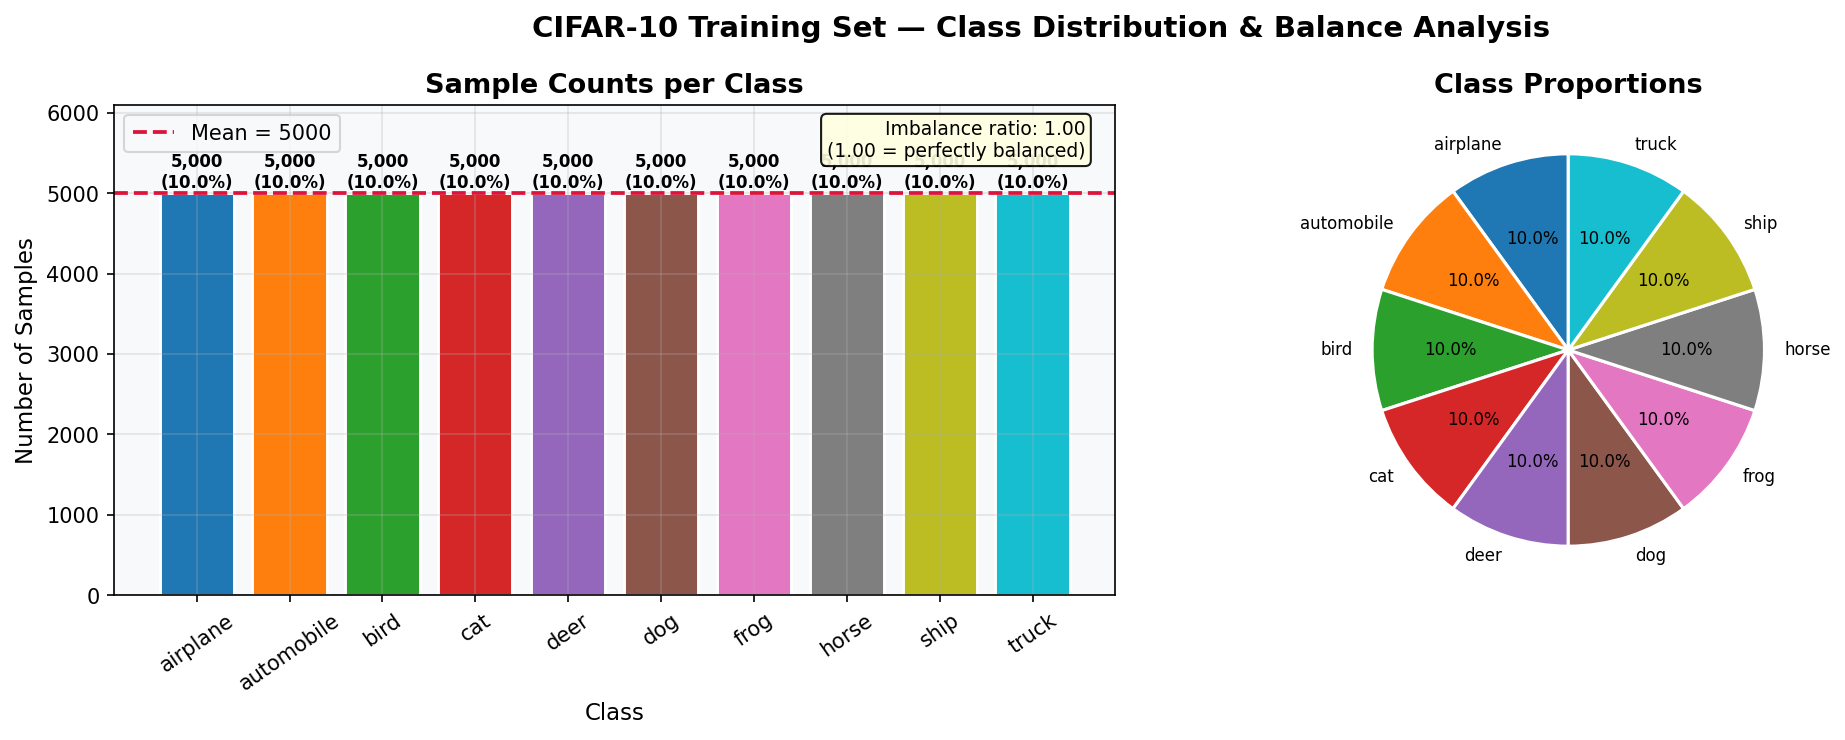
\includegraphics[width=0.85\textwidth]{figures/fig02_class_distribution.png}
\caption{Class distribution of the CIFAR-10 training set (5{,}000 images per class).}
\label{fig:class_dist}
\end{figure}

\begin{figure}[H]
\centering
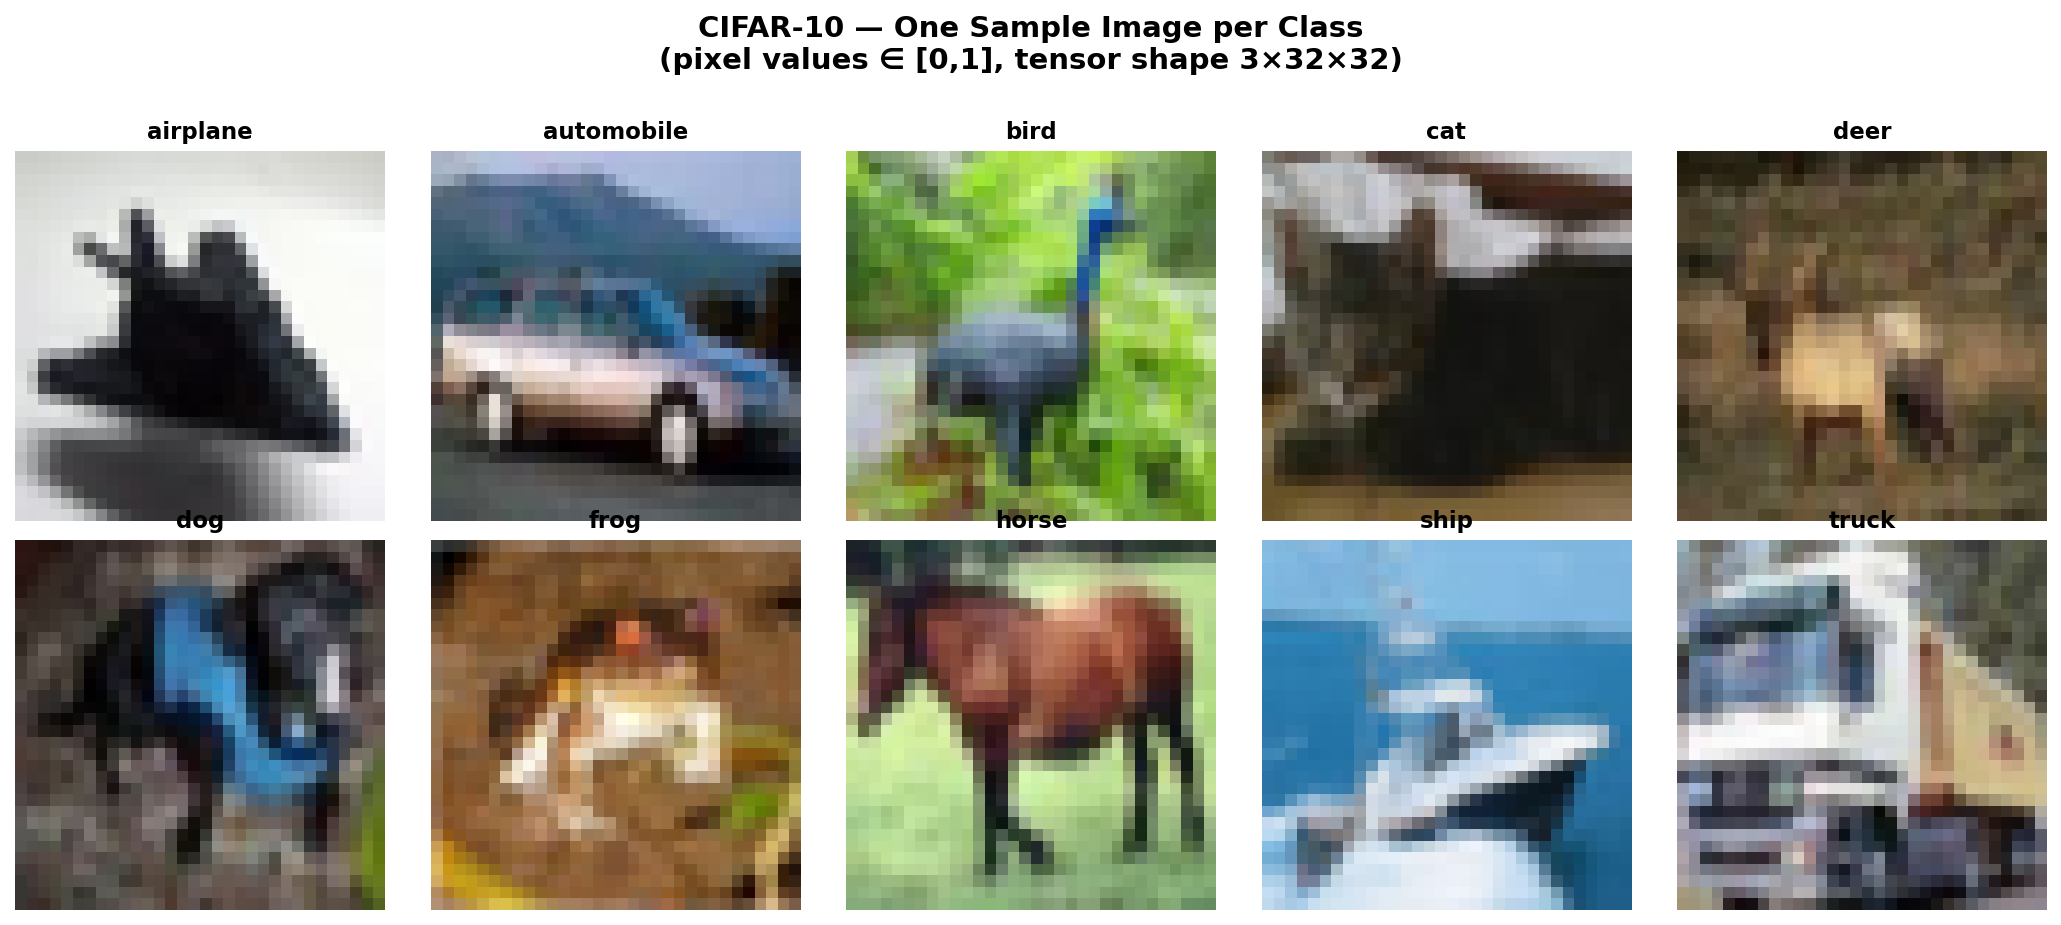
\includegraphics[width=0.85\textwidth]{figures/fig01_cifar10_samples.png}
\caption{Sample images from each of the 10 CIFAR-10 classes.}
\label{fig:samples}
\end{figure}

\begin{figure}[H]
\centering
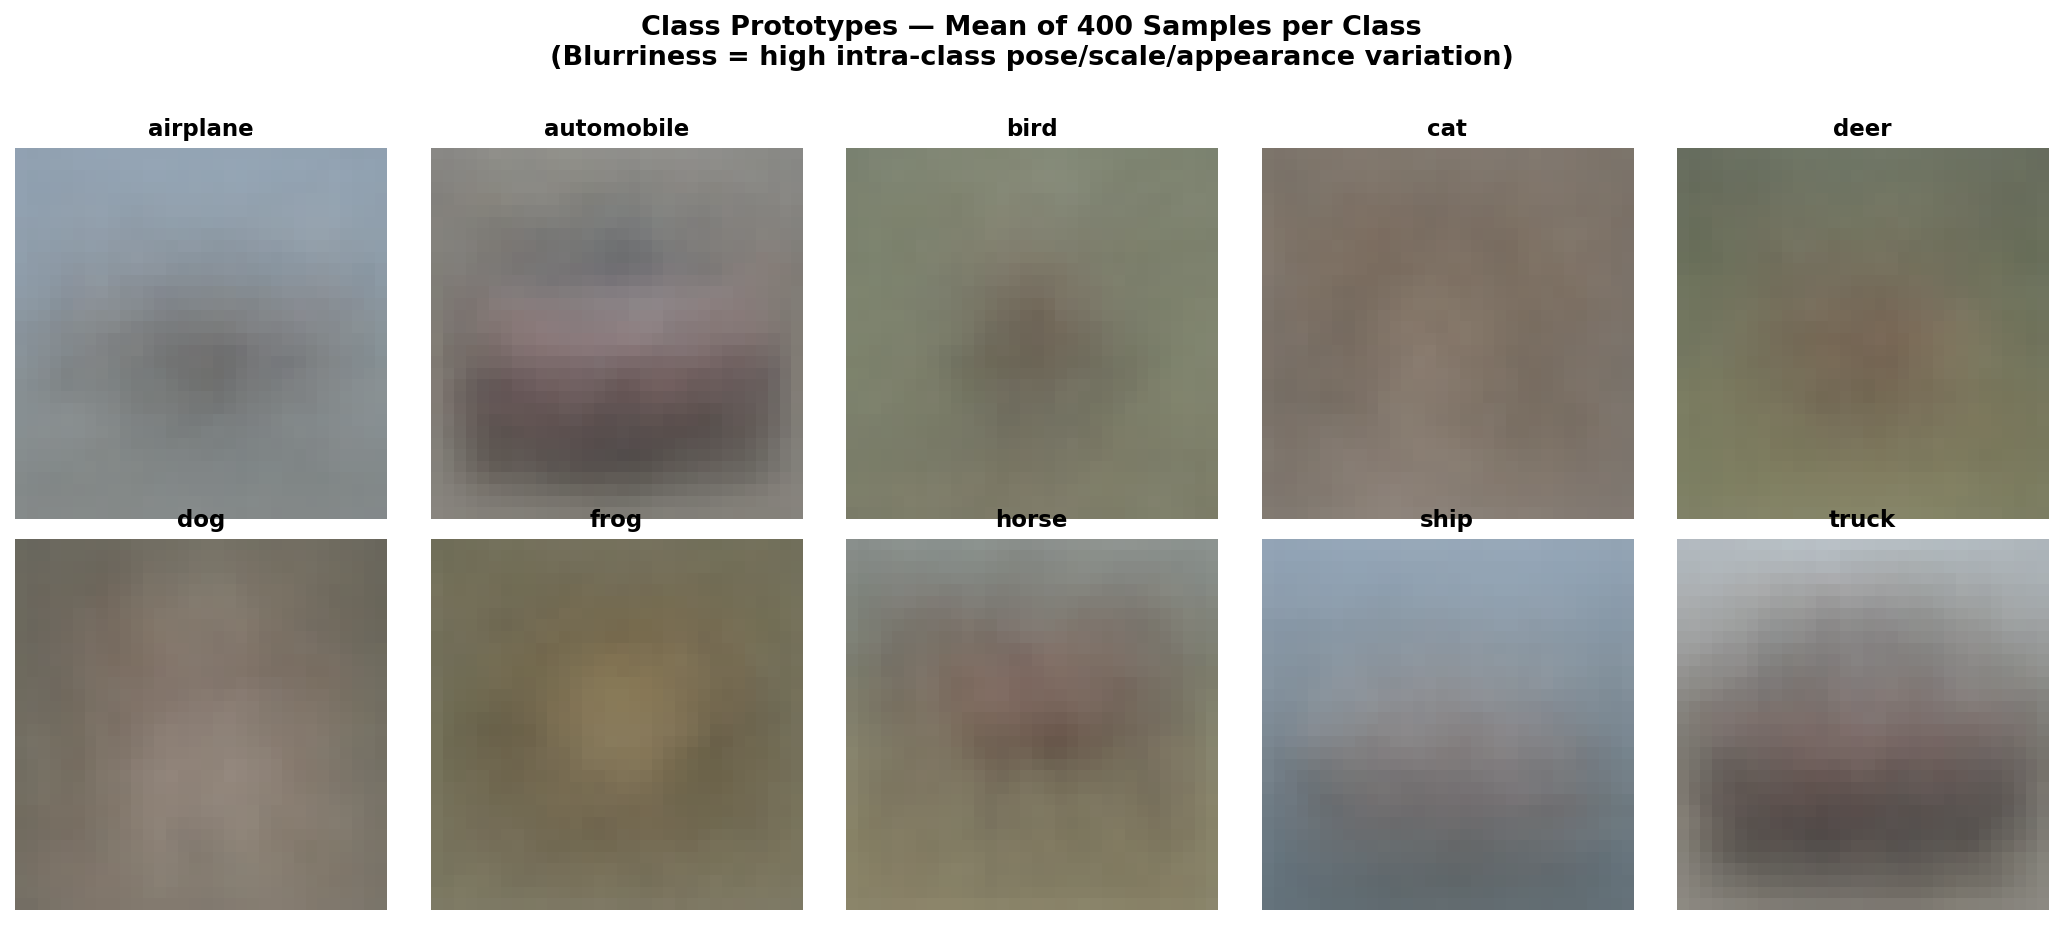
\includegraphics[width=0.85\textwidth]{figures/fig04_class_prototypes.png}
\caption{Mean (prototype) images for each of the 10 CIFAR-10 classes, computed by averaging all training images per class. These prototypes reveal the dominant spatial structure and color distribution characteristic of each category.}
\label{fig:class_prototypes}
\end{figure}

\begin{figure}[H]
\centering
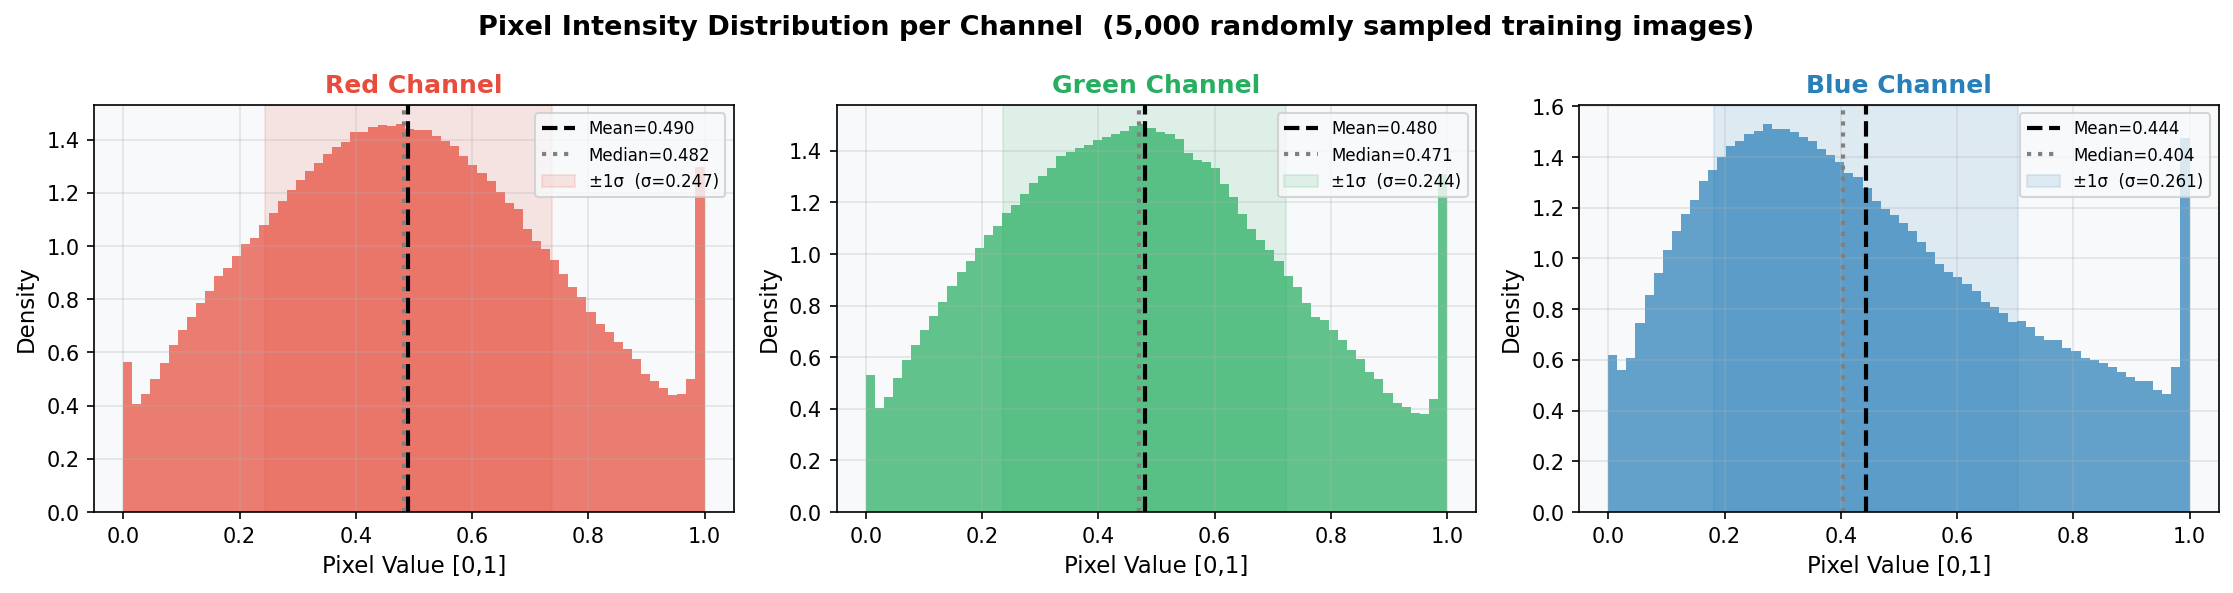
\includegraphics[width=0.80\textwidth]{figures/fig03_pixel_histograms.png}
\caption{Per-channel pixel value histograms for the training set. The Red and Green channels are centered near 125, while the Blue channel is slightly left-shifted, reflecting the natural color bias in CIFAR-10 images.}
\label{fig:pixel_histograms}
\end{figure}


% ─────────────────────────────────────────────────────────────────────────
% 3. CIFAR-10 STATISTICAL ANALYSIS
% ─────────────────────────────────────────────────────────────────────────
\section{CIFAR-10 Statistical Analysis}
\label{sec:statistics}

A comprehensive statistical analysis of the CIFAR-10 dataset was conducted to understand the data characteristics before building the denoising model. This analysis covers descriptive statistics, distribution testing, inter-channel correlations, and dimensionality reduction.

\subsection{Descriptive Statistics}

\subsubsection{Per-Class Statistics}
Figure~\ref{fig:stat_perclass_heatmap} presents a heatmap of descriptive statistics (mean, standard deviation, median, IQR, skewness, kurtosis, and coefficient of variation) computed per class. Notable observations include:
\begin{itemize}[nosep]
    \item \textbf{Frog} class has the highest mean pixel value due to dominant green backgrounds.
    \item \textbf{Cat} and \textbf{dog} classes exhibit the highest standard deviations, reflecting their diverse appearance patterns.
    \item All classes show right-skewed (positive skewness) pixel distributions with negative excess kurtosis (platykurtic, i.e., lighter tails than Gaussian).
\end{itemize}

\begin{figure}[H]
\centering
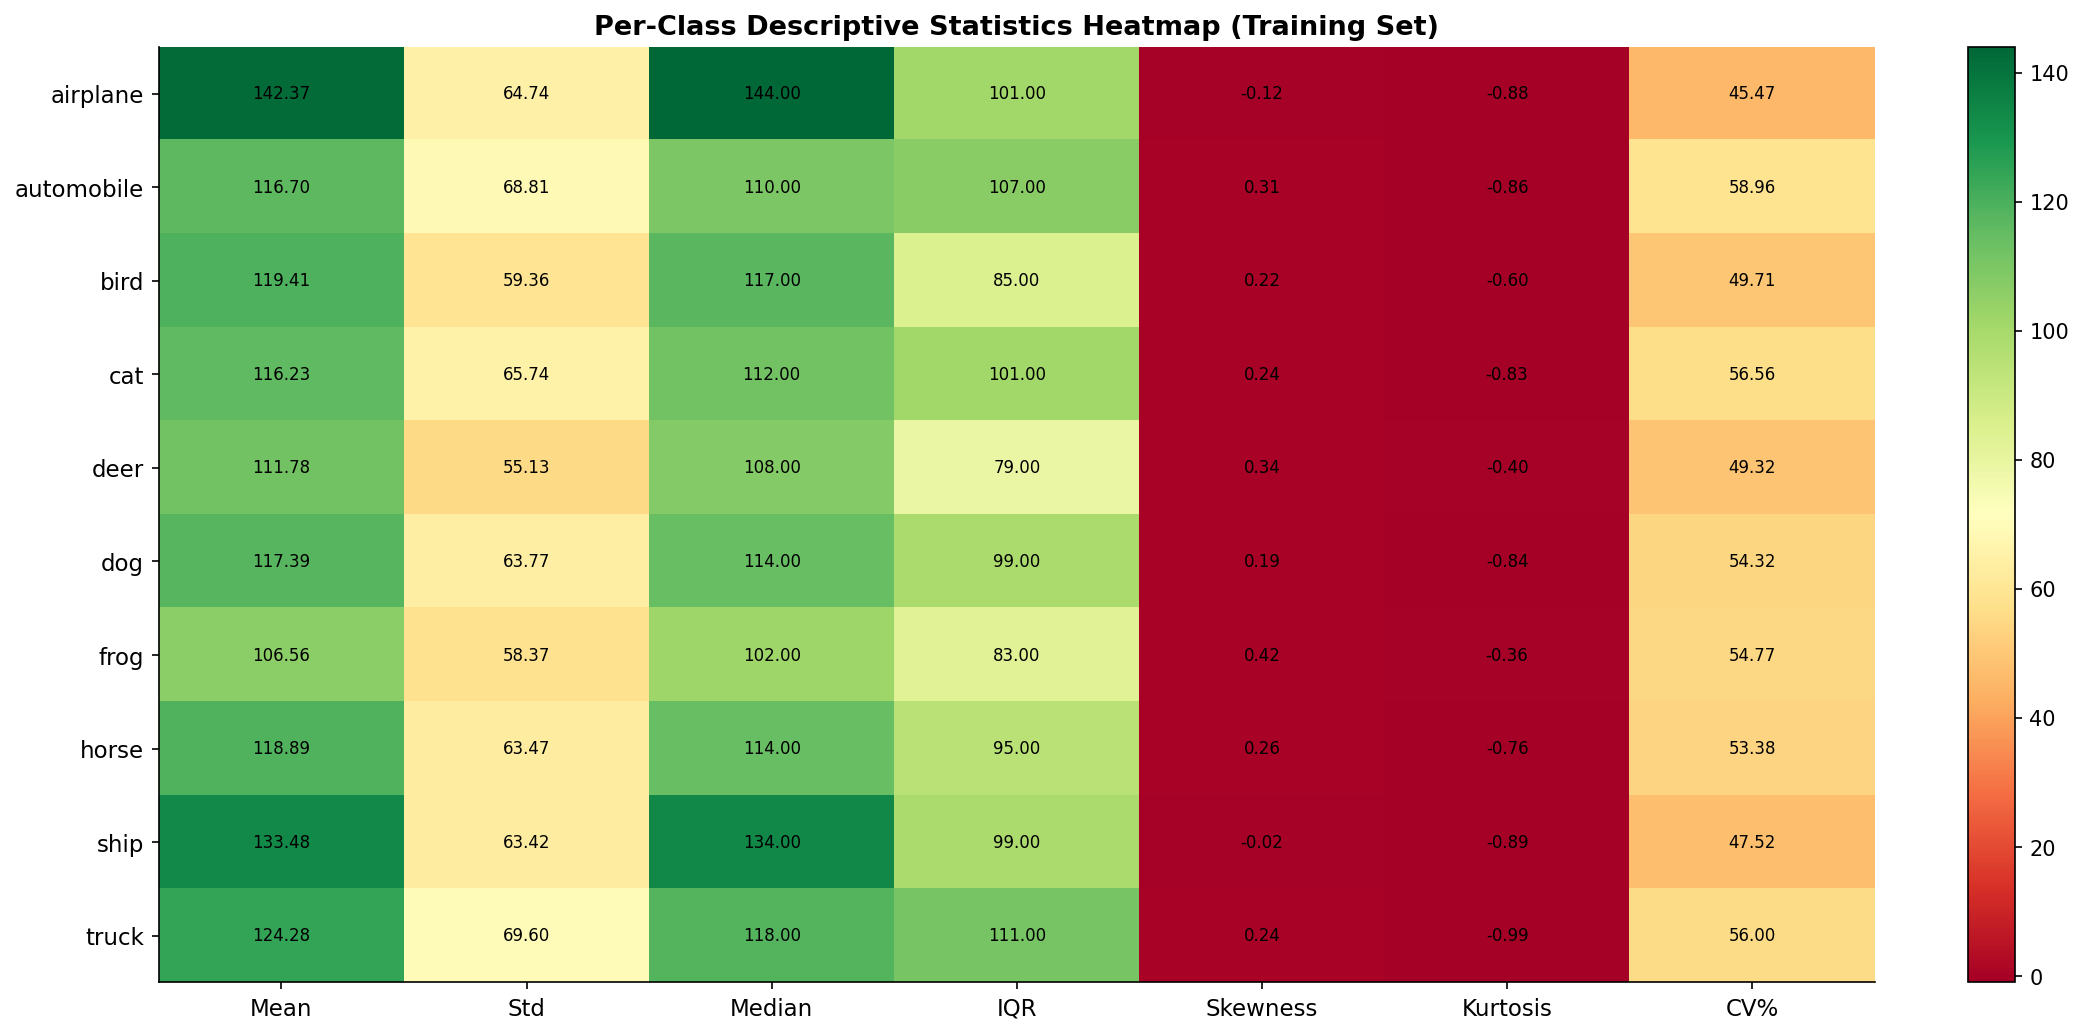
\includegraphics[width=0.90\textwidth]{figures/stat01_perclass_heatmap.png}
\caption{Per-class descriptive statistics heatmap. Each row represents a CIFAR-10 class, and columns show different statistical metrics. Color intensity encodes the metric value across classes.}
\label{fig:stat_perclass_heatmap}
\end{figure}

\subsubsection{Image-Level Brightness and Contrast}
Figure~\ref{fig:stat_brightness} shows the distributions of per-image brightness (mean pixel value) and contrast (standard deviation of pixel values), along with their per-class breakdown. There is a moderate negative correlation between brightness and contrast, and different classes occupy distinct regions of the brightness-contrast space.

\begin{figure}[H]
\centering
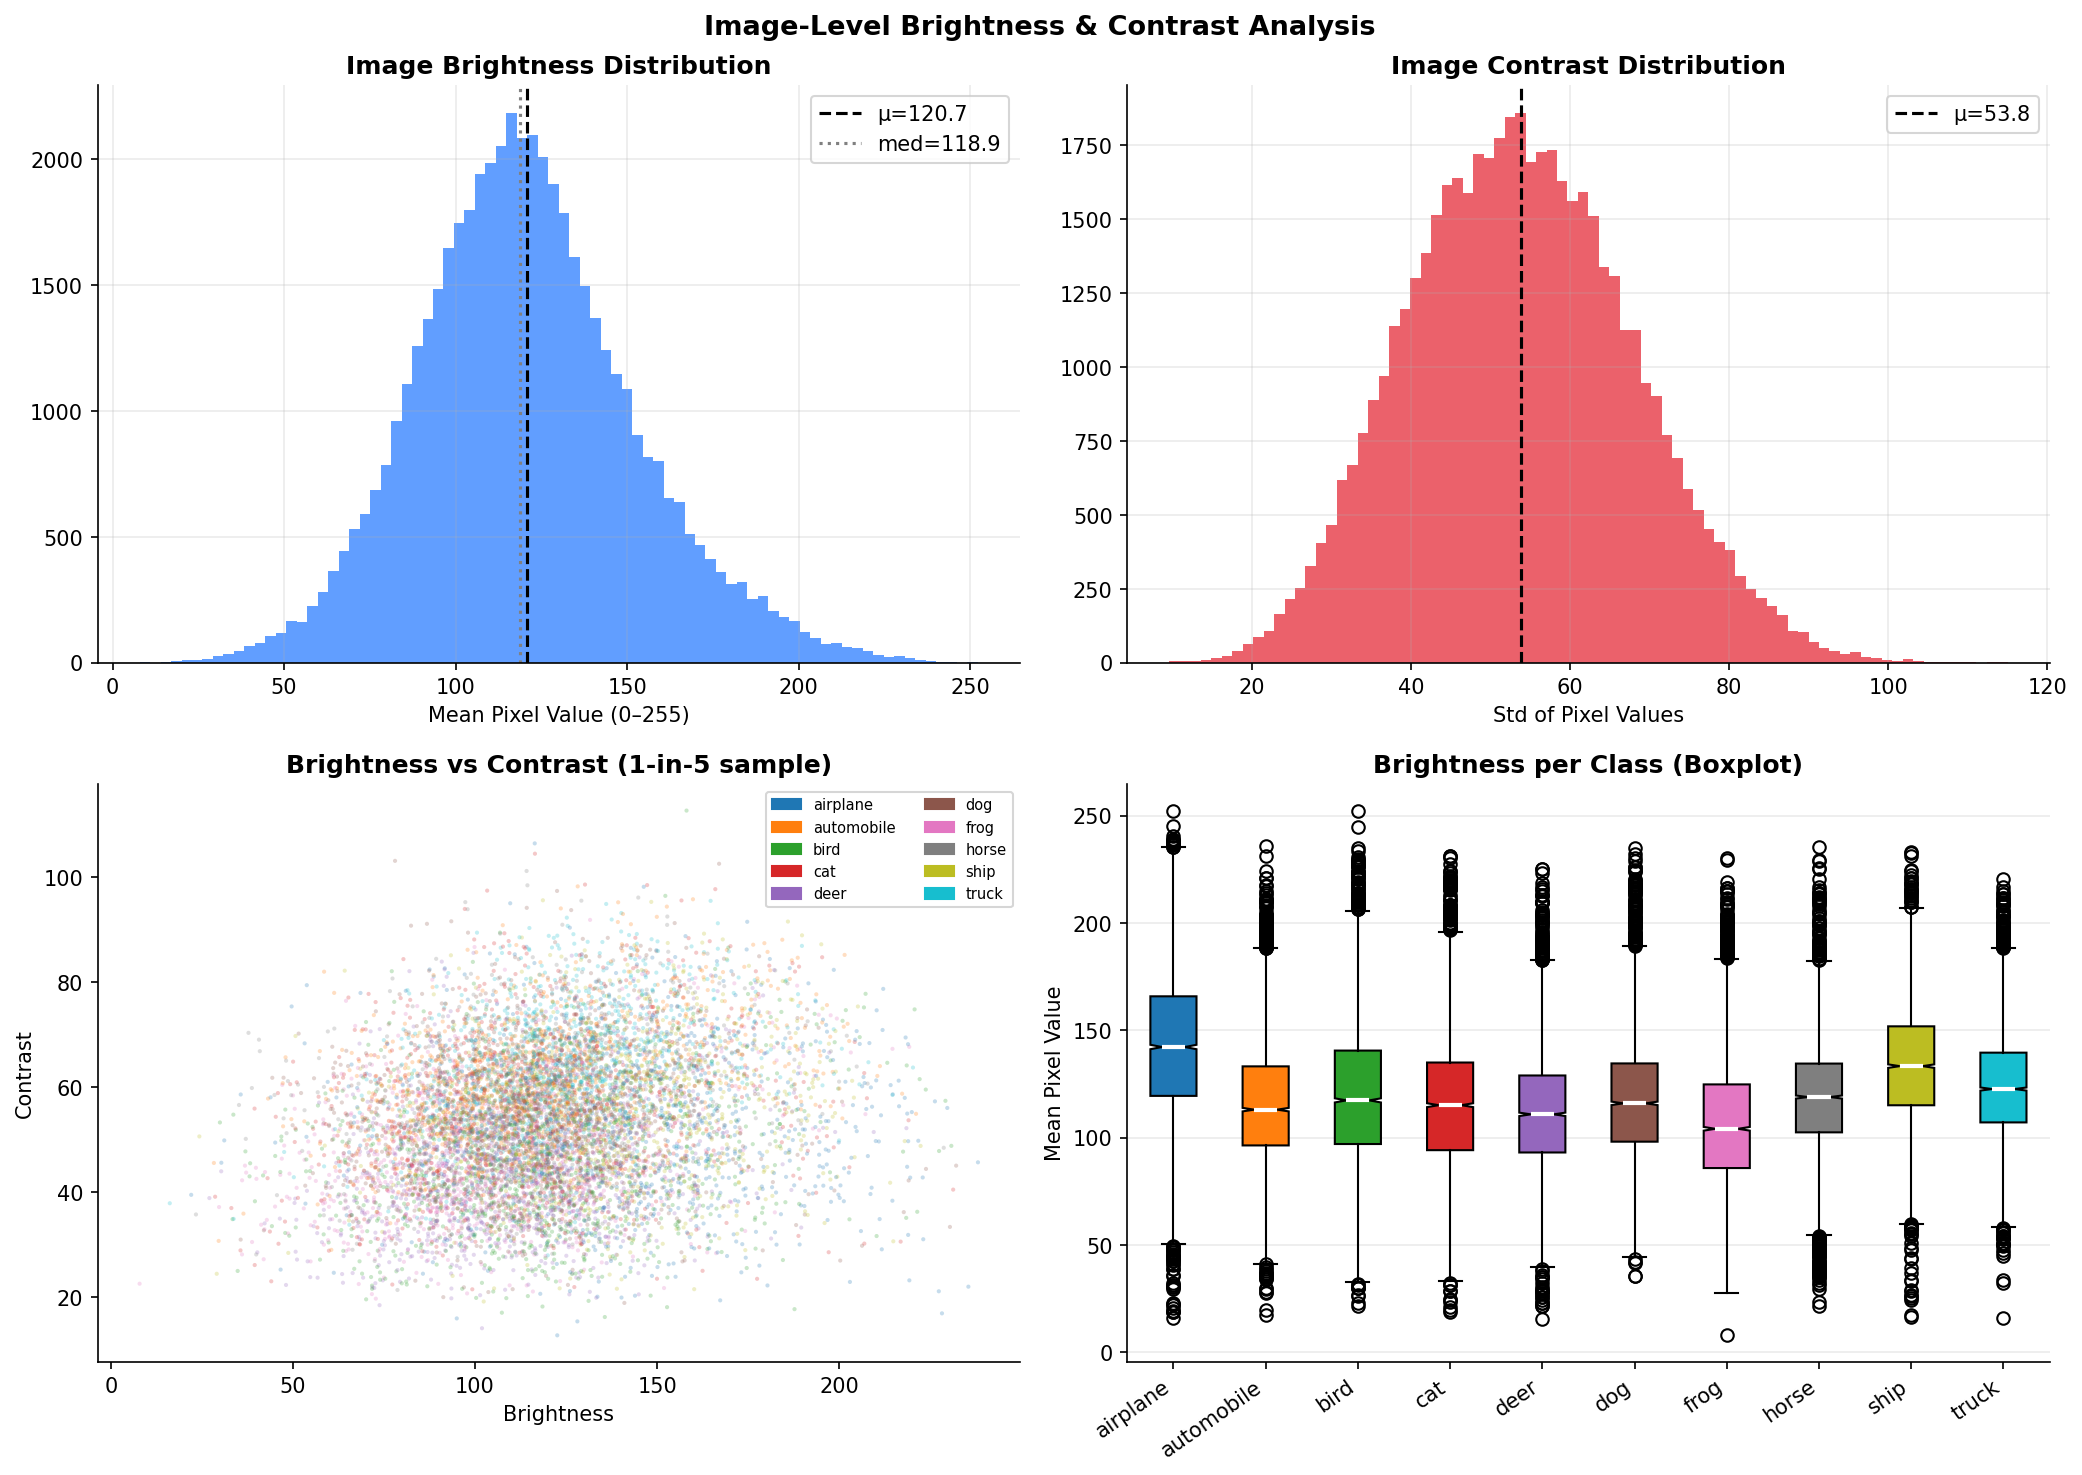
\includegraphics[width=0.95\textwidth]{figures/stat01_brightness_contrast.png}
\caption{Image-level brightness and contrast analysis. Top-left: brightness histogram. Top-right: contrast histogram. Bottom-left: brightness vs.\ contrast scatter plot colored by class. Bottom-right: per-class brightness boxplot.}
\label{fig:stat_brightness}
\end{figure}

\subsubsection{Percentile Analysis}
Figure~\ref{fig:stat_percentiles} shows the quantile functions for each color channel. The curves reveal that the Red channel has a wider interquartile range than the Blue channel, and that extreme pixel values (near 0 or 255) are relatively rare.

\begin{figure}[H]
\centering
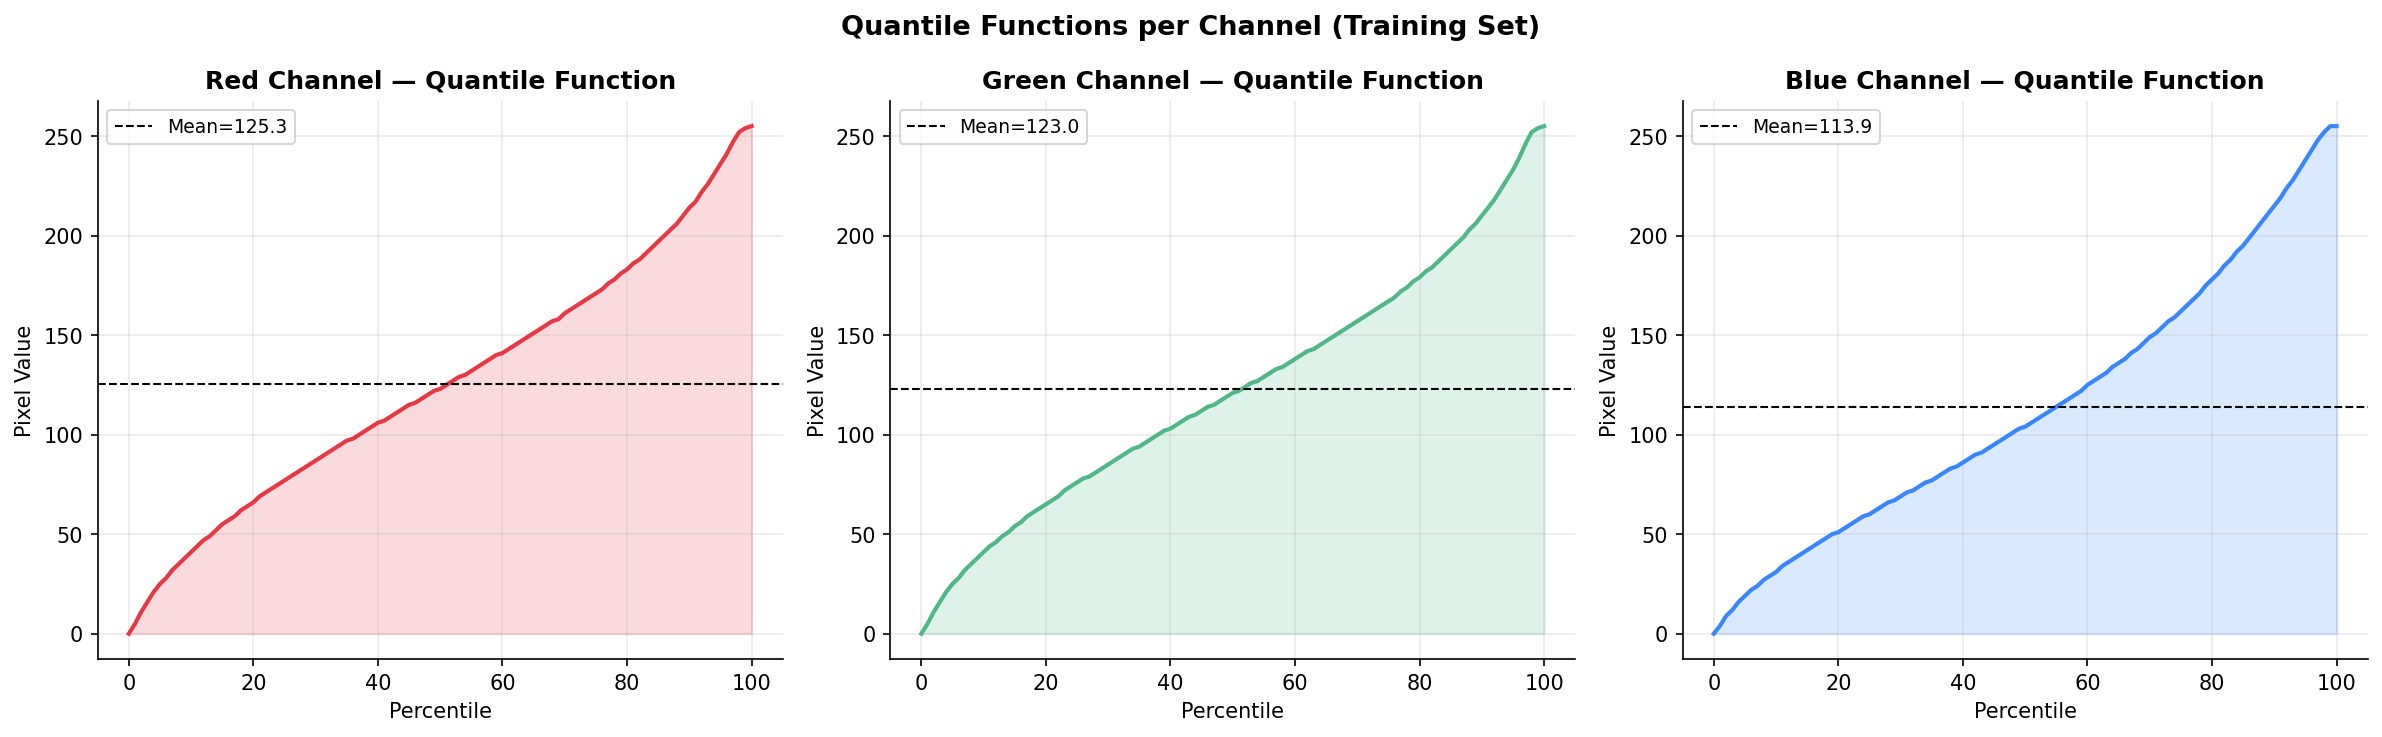
\includegraphics[width=0.90\textwidth]{figures/stat01_percentiles.png}
\caption{Quantile functions per channel (training set). The shaded area under each curve represents the full distribution of pixel values from the 0th to 100th percentile.}
\label{fig:stat_percentiles}
\end{figure}

\subsubsection{Spatial Variance Maps}
Figure~\ref{fig:stat_spatial} shows per-pixel mean and standard deviation maps averaged across all training images. The center of each 32$\times$32 map tends to have higher variance (where objects appear), while edges are more uniform (often sky or background).

\begin{figure}[H]
\centering
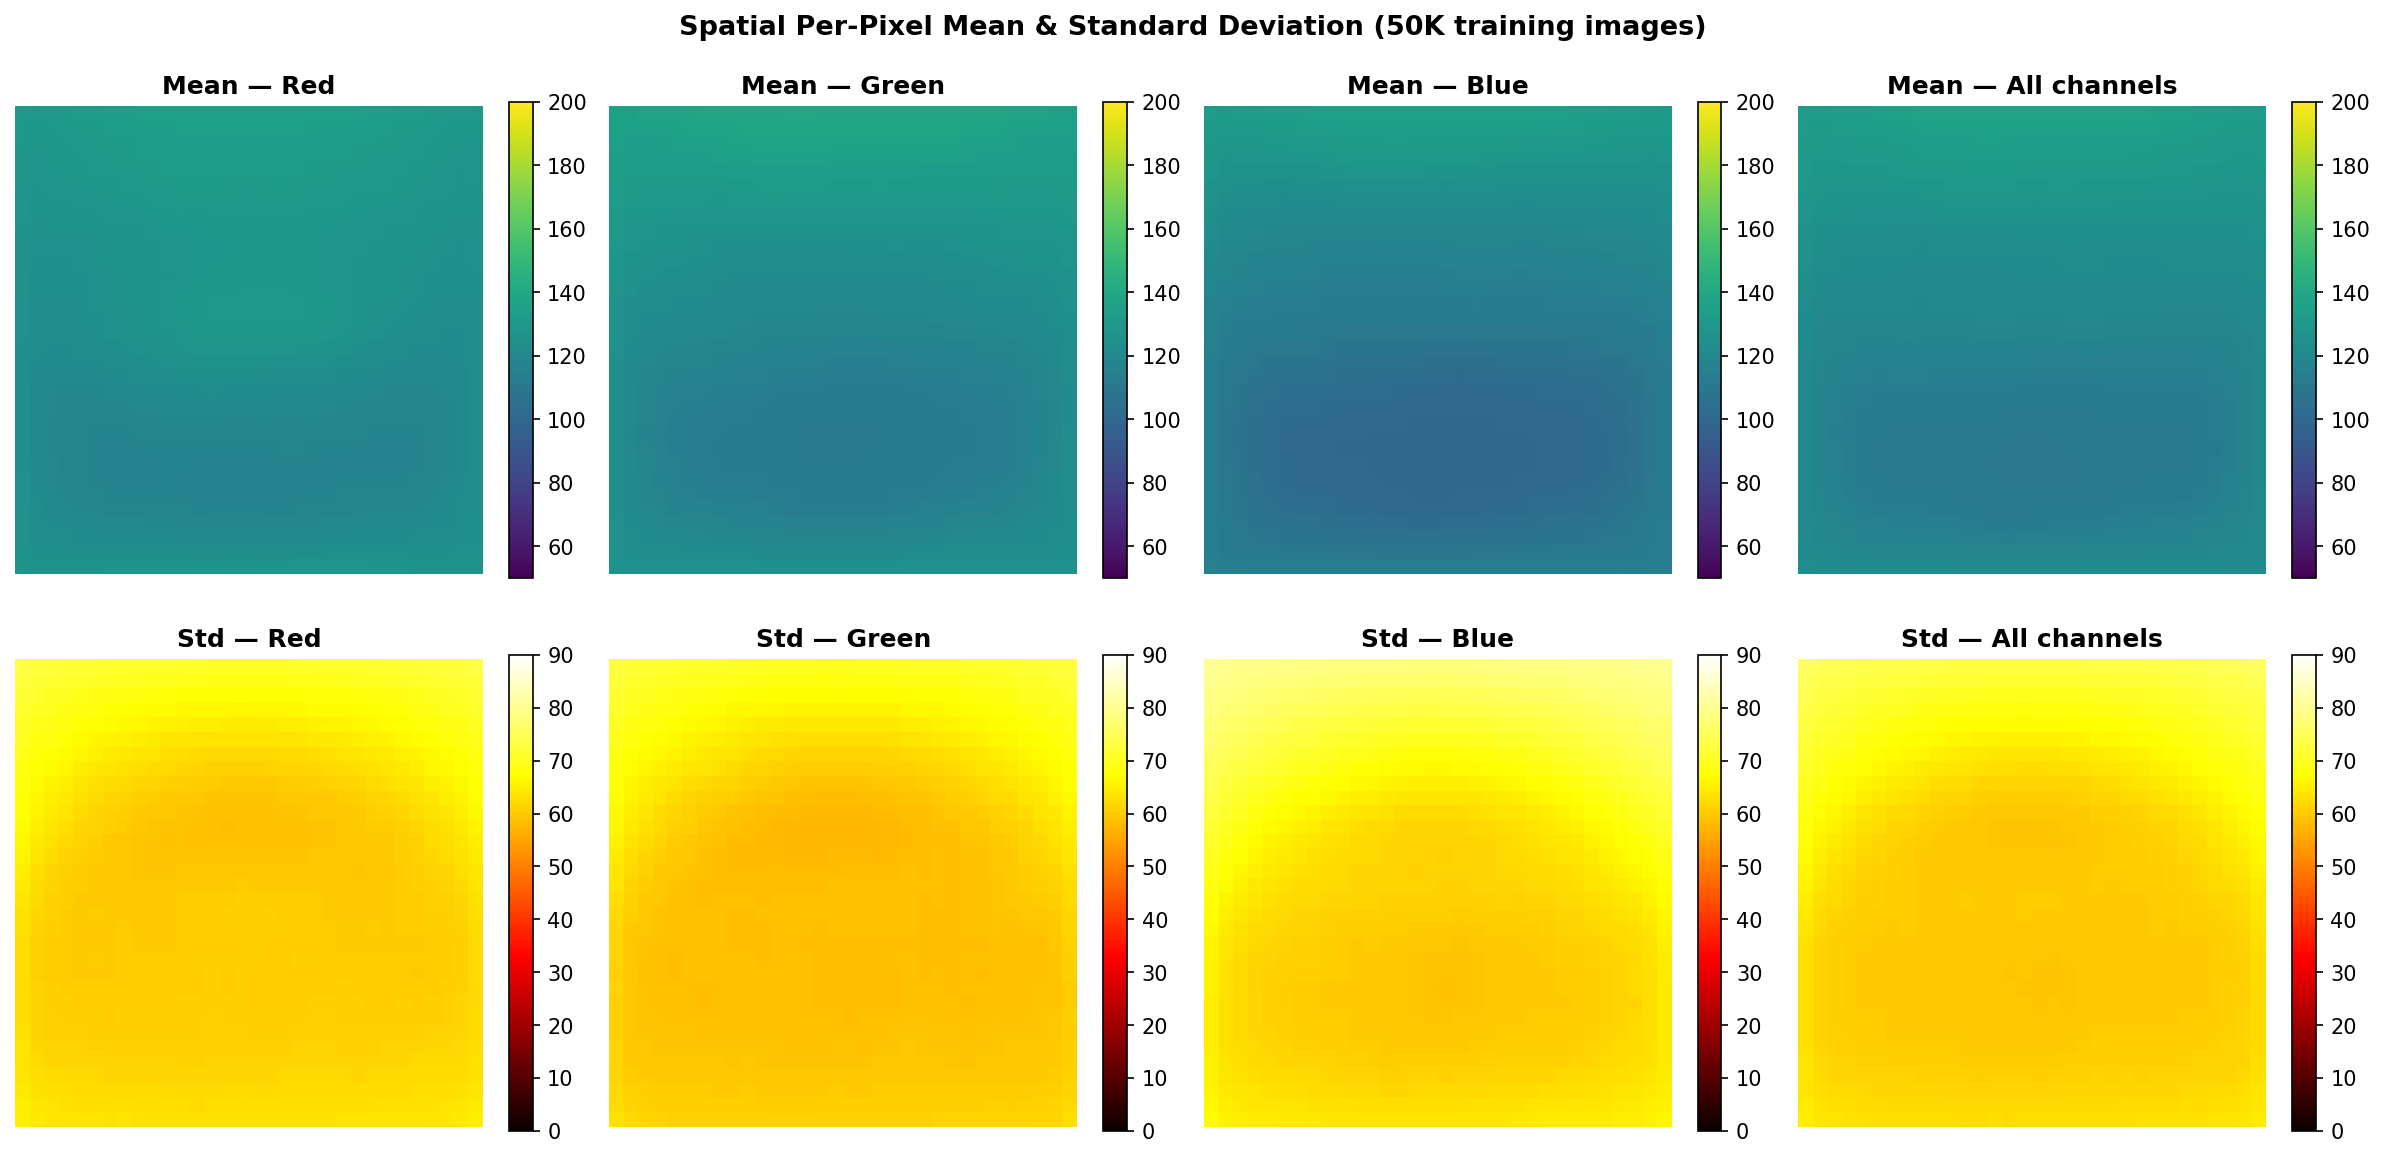
\includegraphics[width=0.95\textwidth]{figures/stat01_spatial_maps.png}
\caption{Spatial per-pixel mean (top) and standard deviation (bottom) maps computed from all 50{,}000 training images. The center shows higher variability, consistent with object-centric compositions.}
\label{fig:stat_spatial}
\end{figure}

\begin{figure}[H]
\centering
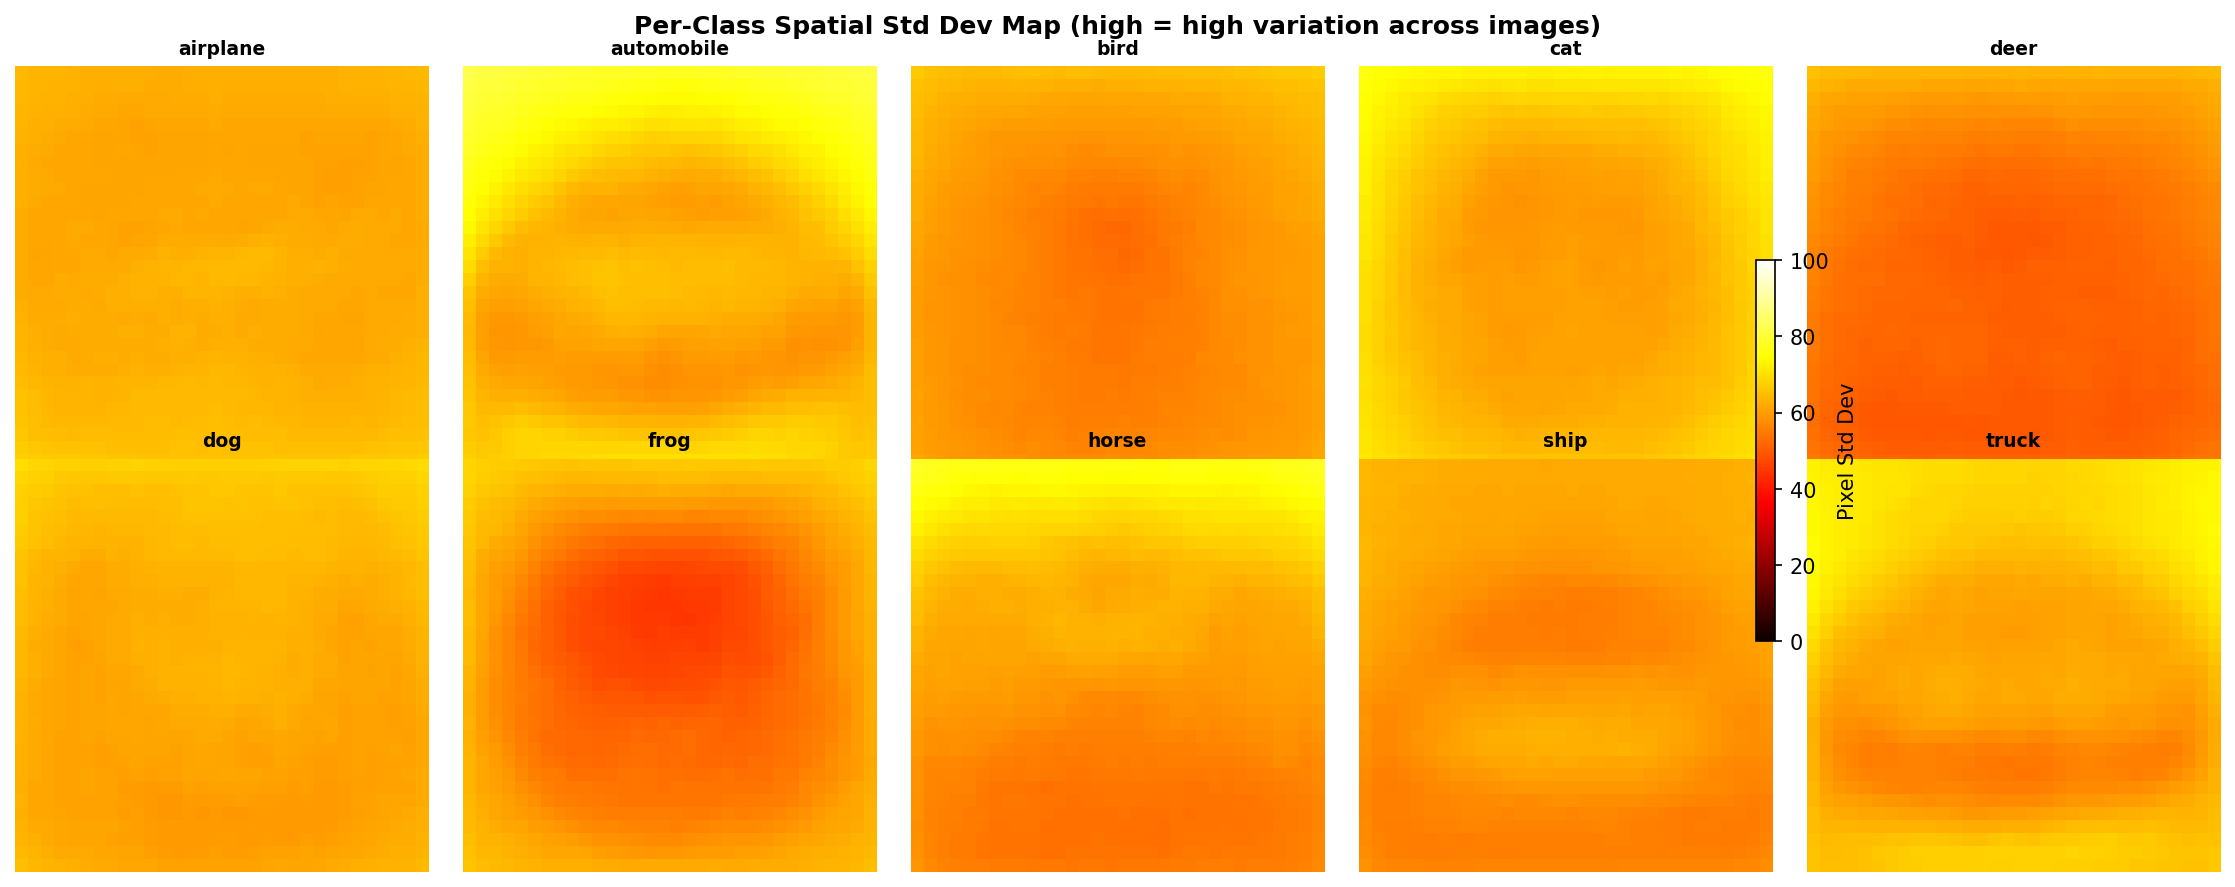
\includegraphics[width=0.90\textwidth]{figures/stat01_perclass_spatial_std.png}
\caption{Per-class spatial standard deviation maps. Each map shows where pixel values vary most within a class. Vehicle classes (airplane, ship) show concentrated central variance, while animal classes show more diffuse patterns.}
\label{fig:stat_spatial_perclass}
\end{figure}

\subsubsection{Coefficient of Variation}
Figure~\ref{fig:stat_cv} shows the coefficient of variation (CV\%) per class and channel. The Blue channel consistently exhibits the highest CV across all classes, indicating it carries the most relative variability.

\begin{figure}[H]
\centering
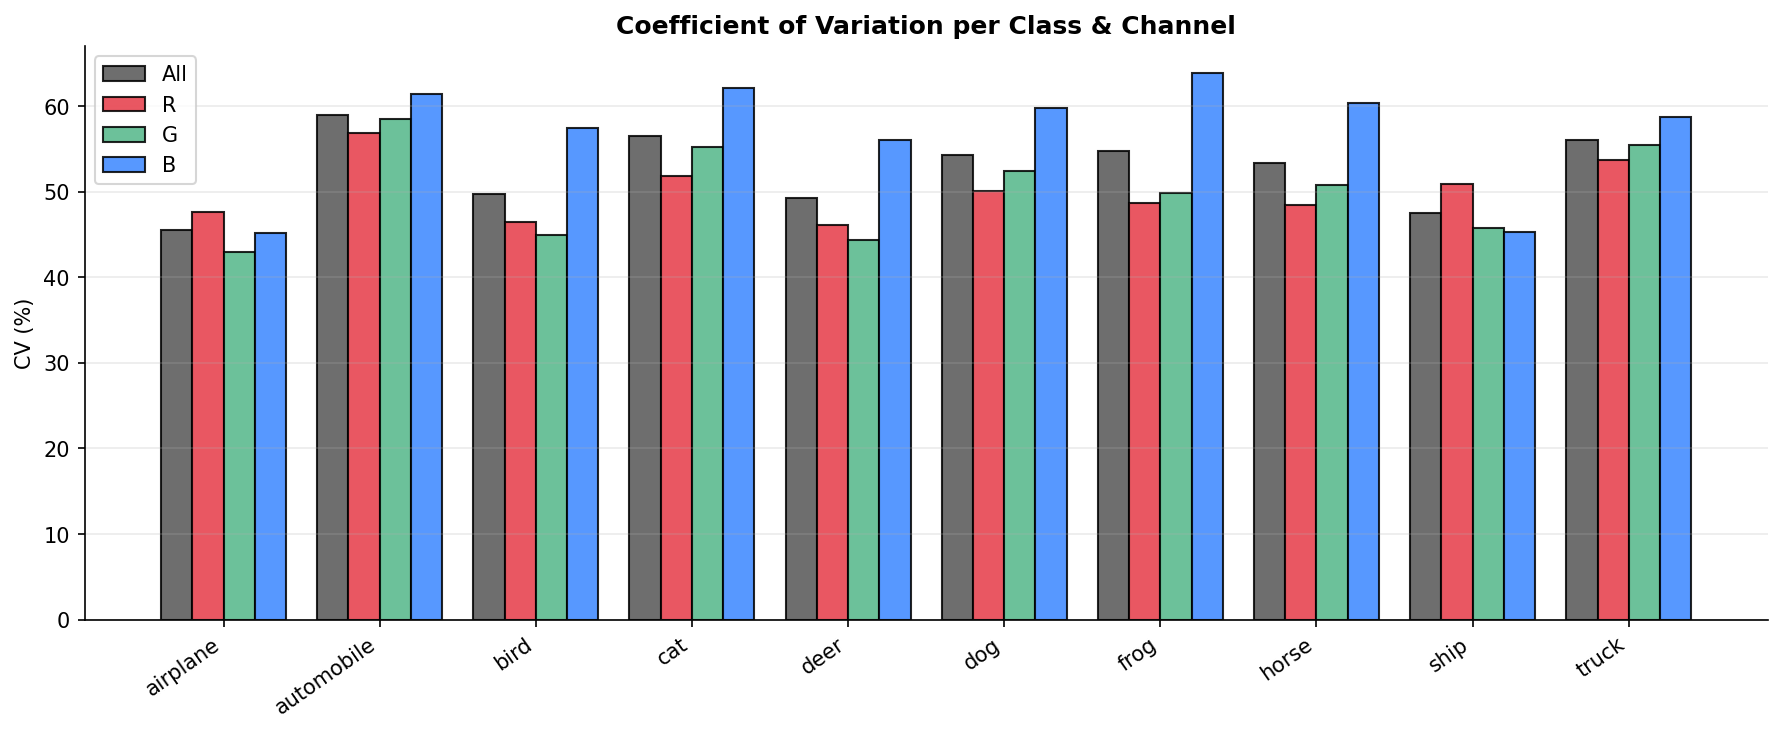
\includegraphics[width=0.85\textwidth]{figures/stat01_cv.png}
\caption{Coefficient of variation (\%) per class and color channel. Higher CV indicates greater relative pixel variability.}
\label{fig:stat_cv}
\end{figure}


\subsection{Distribution Analysis}

\subsubsection{Pixel Value Distributions}
Figure~\ref{fig:stat_histograms} overlays the empirical pixel histograms with fitted Normal distributions and Kernel Density Estimates (KDE) for each channel across both training and test splits.

\begin{figure}[H]
\centering
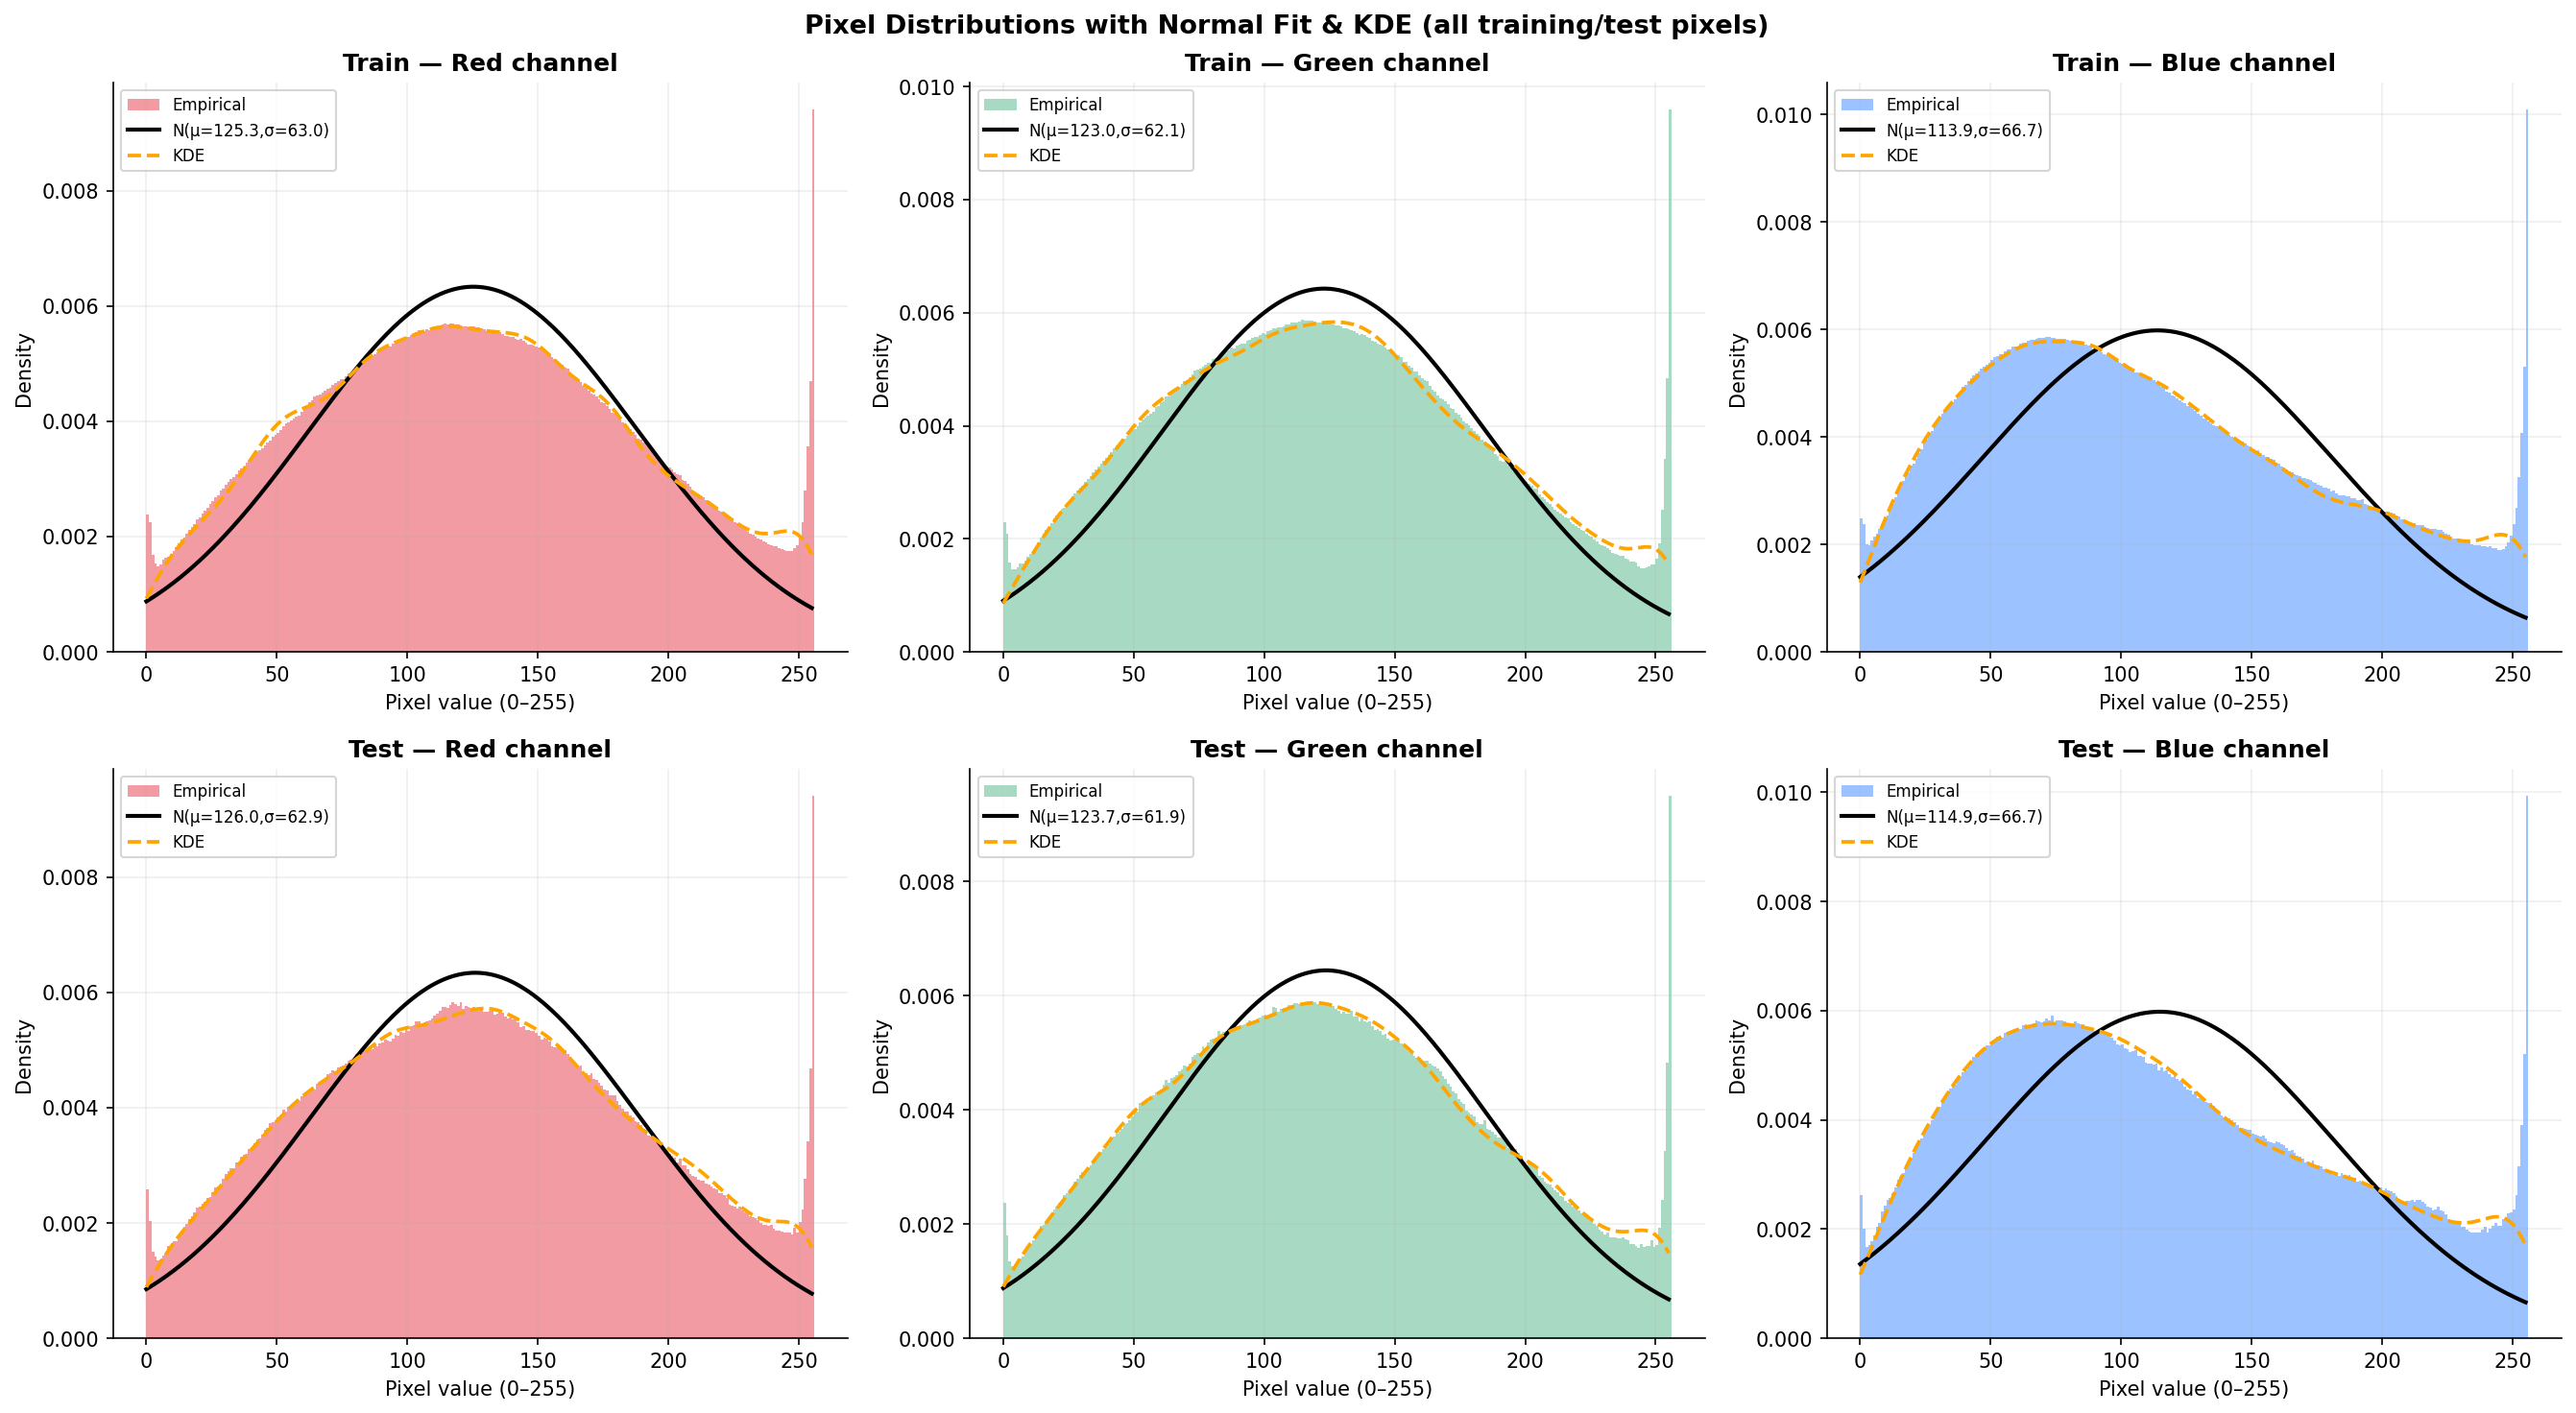
\includegraphics[width=0.95\textwidth]{figures/stat02_histograms_fitted.png}
\caption{Pixel value histograms with fitted Normal distribution and KDE. Top row: training set. Bottom row: test set. The bimodal shape (peaks near 0 and 128) indicates that CIFAR-10 pixels deviate significantly from normality.}
\label{fig:stat_histograms}
\end{figure}

\subsubsection{Q-Q Plots}
Figure~\ref{fig:stat_qq} presents Normal Q-Q plots for each channel. The systematic S-shaped deviation from the diagonal confirms the non-normality observed in the histograms.

\begin{figure}[H]
\centering
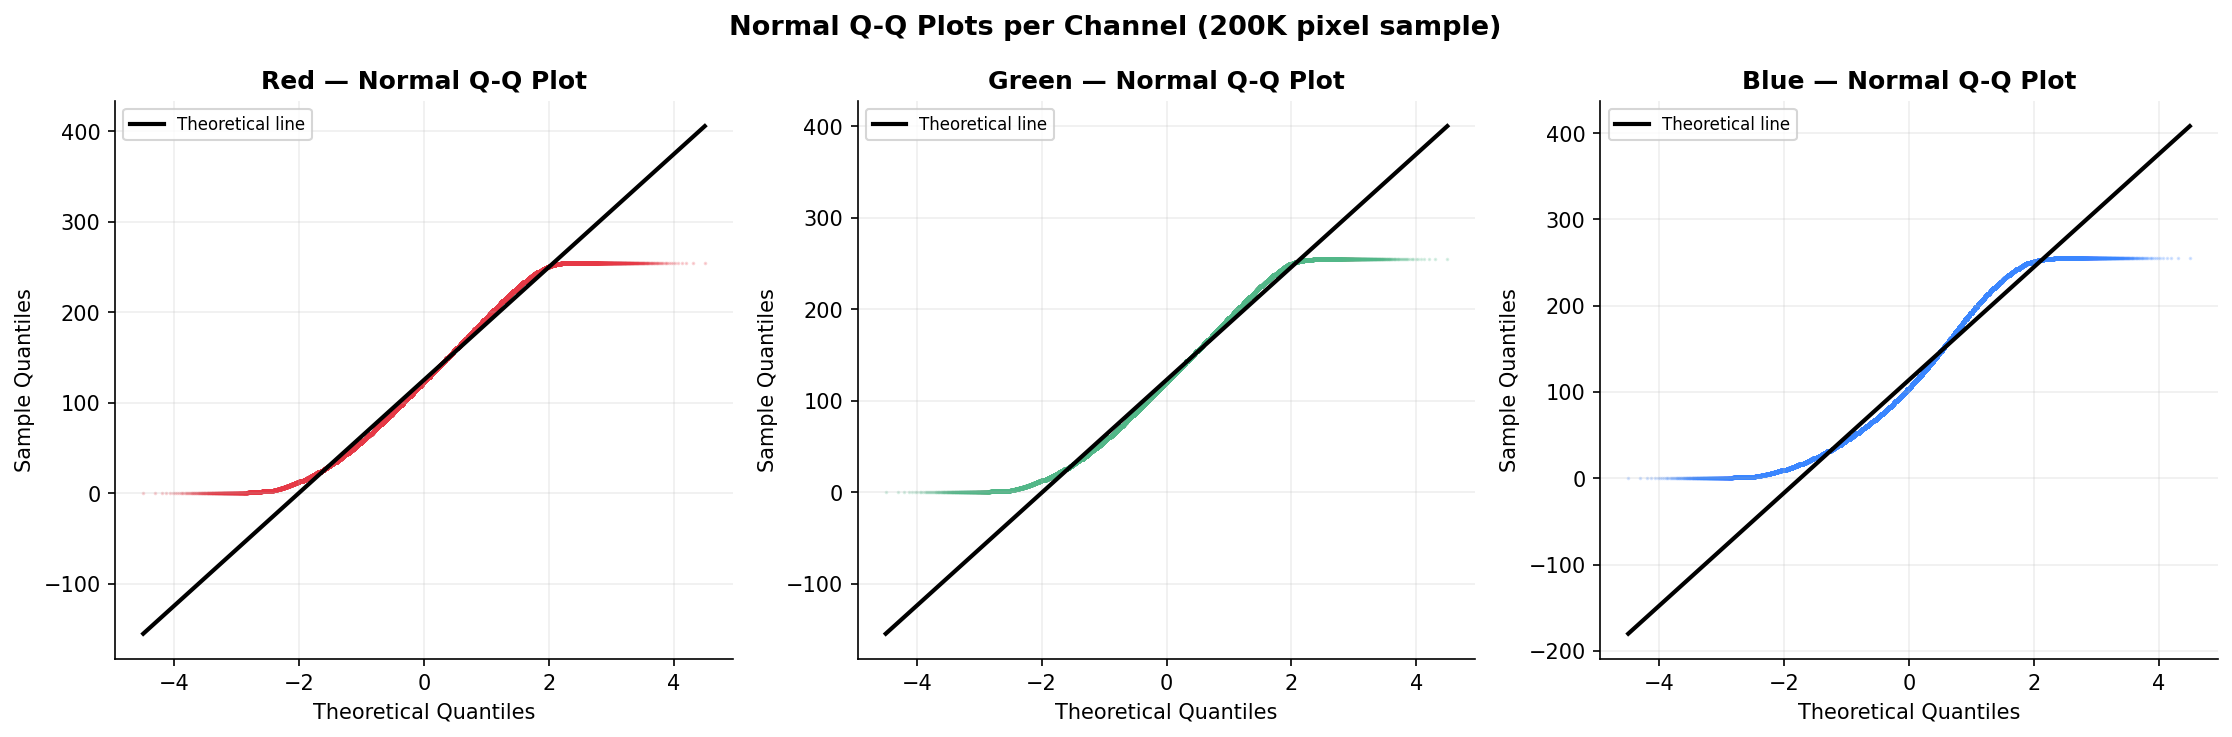
\includegraphics[width=0.90\textwidth]{figures/stat02_qqplots.png}
\caption{Normal Q-Q plots per channel (200K pixel sample). Deviations from the diagonal line indicate departure from normality, with heavy tails evident at both extremes.}
\label{fig:stat_qq}
\end{figure}

\subsubsection{Train vs.\ Test Distribution Comparison}
Figure~\ref{fig:stat_train_test} overlays the KDE distributions of the training and test splits per channel. The near-perfect overlap confirms that the train/test split preserves the original data distribution.

\begin{figure}[H]
\centering
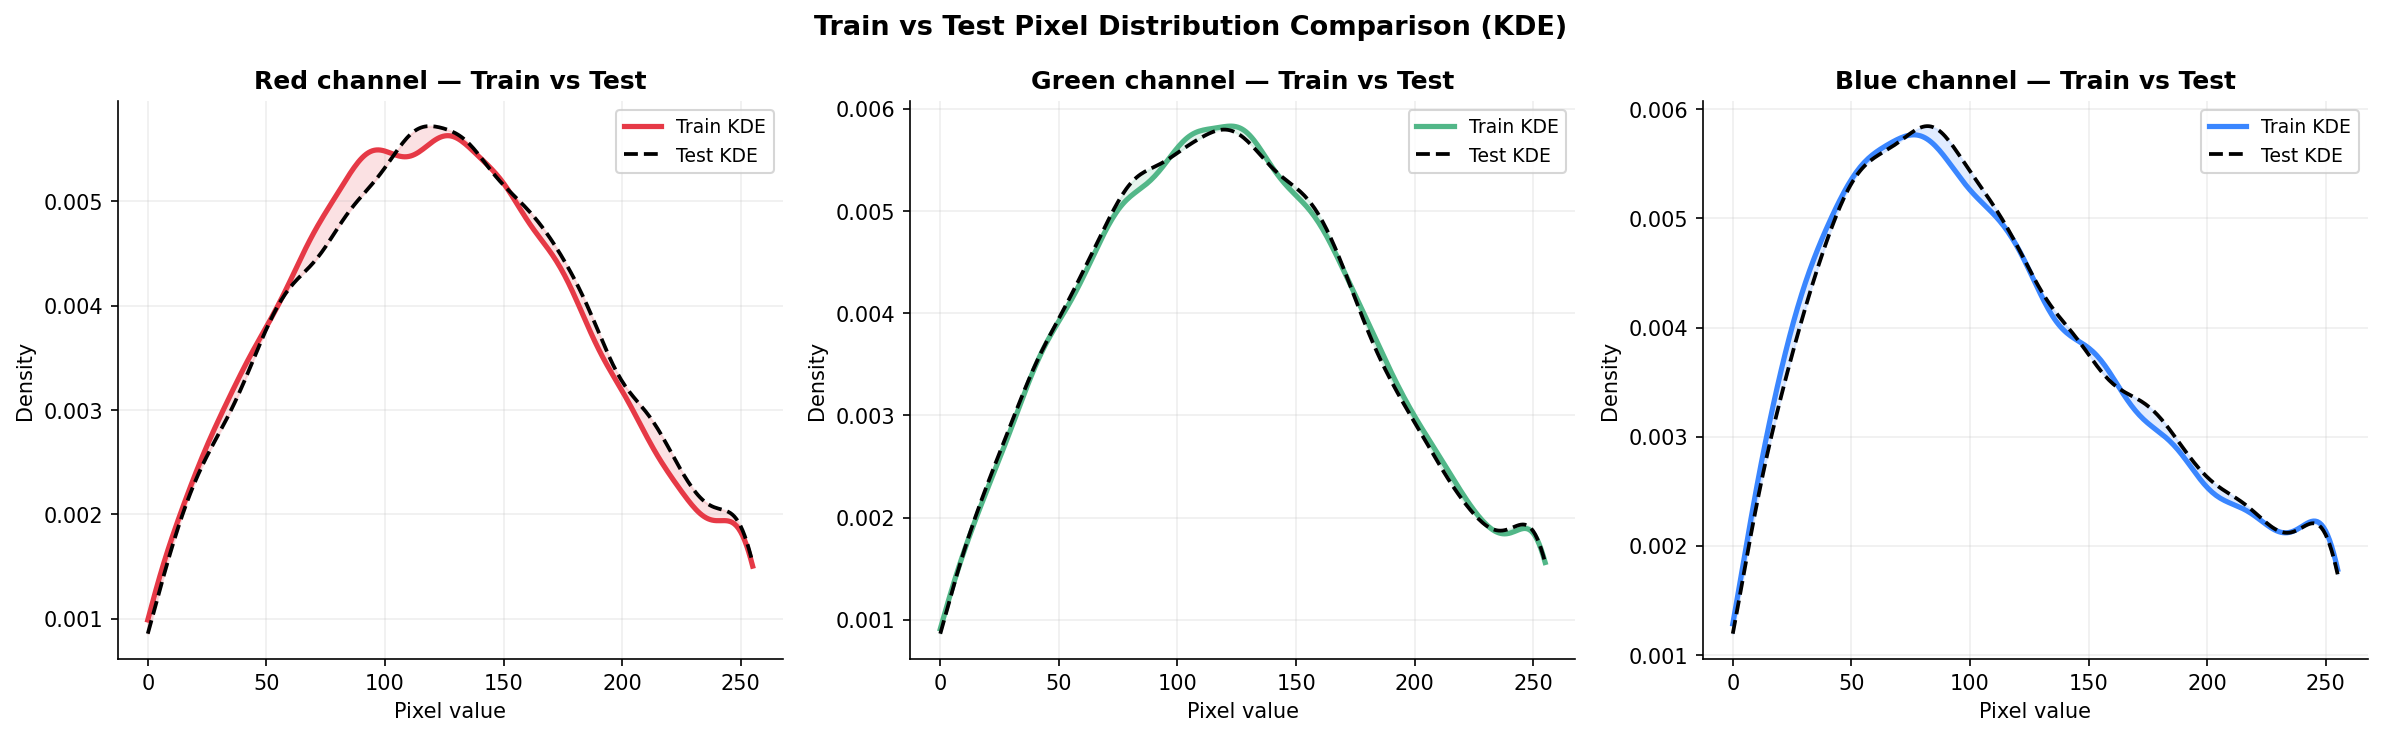
\includegraphics[width=0.90\textwidth]{figures/stat02_train_vs_test.png}
\caption{Train vs.\ Test pixel distribution comparison using KDE. The close overlay between training (solid) and test (dashed) curves validates the dataset split consistency.}
\label{fig:stat_train_test}
\end{figure}

\subsubsection{Per-Class Distribution}
Figure~\ref{fig:stat_kde_class} shows KDE overlays per class for each channel. Classes like ``frog'' and ``deer'' dominate higher pixel values (green-shifted), while ``automobile'' and ``truck'' peak at darker values.

\begin{figure}[H]
\centering
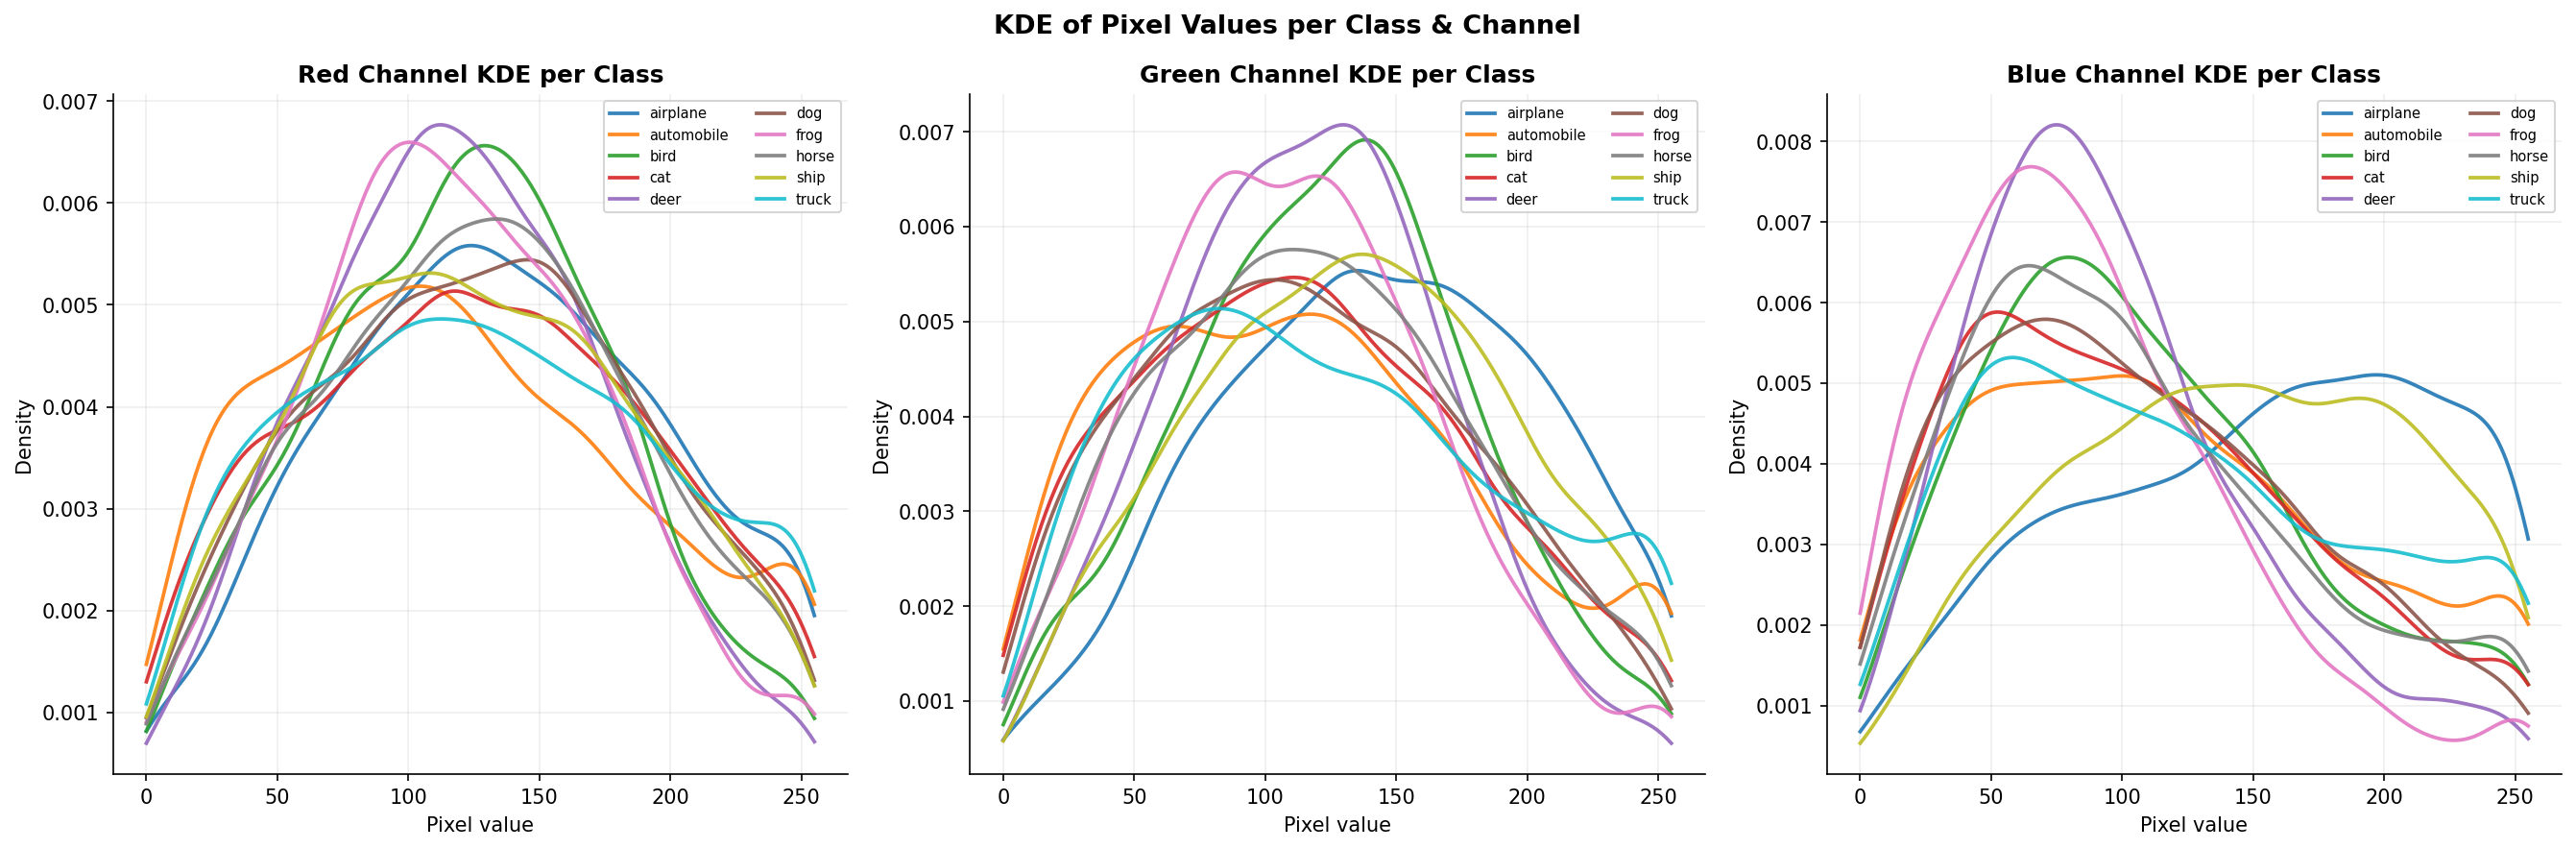
\includegraphics[width=0.95\textwidth]{figures/stat02_kde_per_class.png}
\caption{KDE of pixel values per class and channel. Each curve represents one CIFAR-10 class. Class-specific color biases are clearly visible, especially for nature vs.\ vehicle categories.}
\label{fig:stat_kde_class}
\end{figure}


\subsection{Correlation Analysis}

\subsubsection{Inter-Channel Correlation}
Figure~\ref{fig:stat_corr_matrix} shows the Pearson correlation matrix between the R, G, and B channels. All channel pairs exhibit strong positive correlations ($r > 0.75$), which is expected for natural color images where brightness variations affect all channels simultaneously.

\begin{figure}[H]
\centering
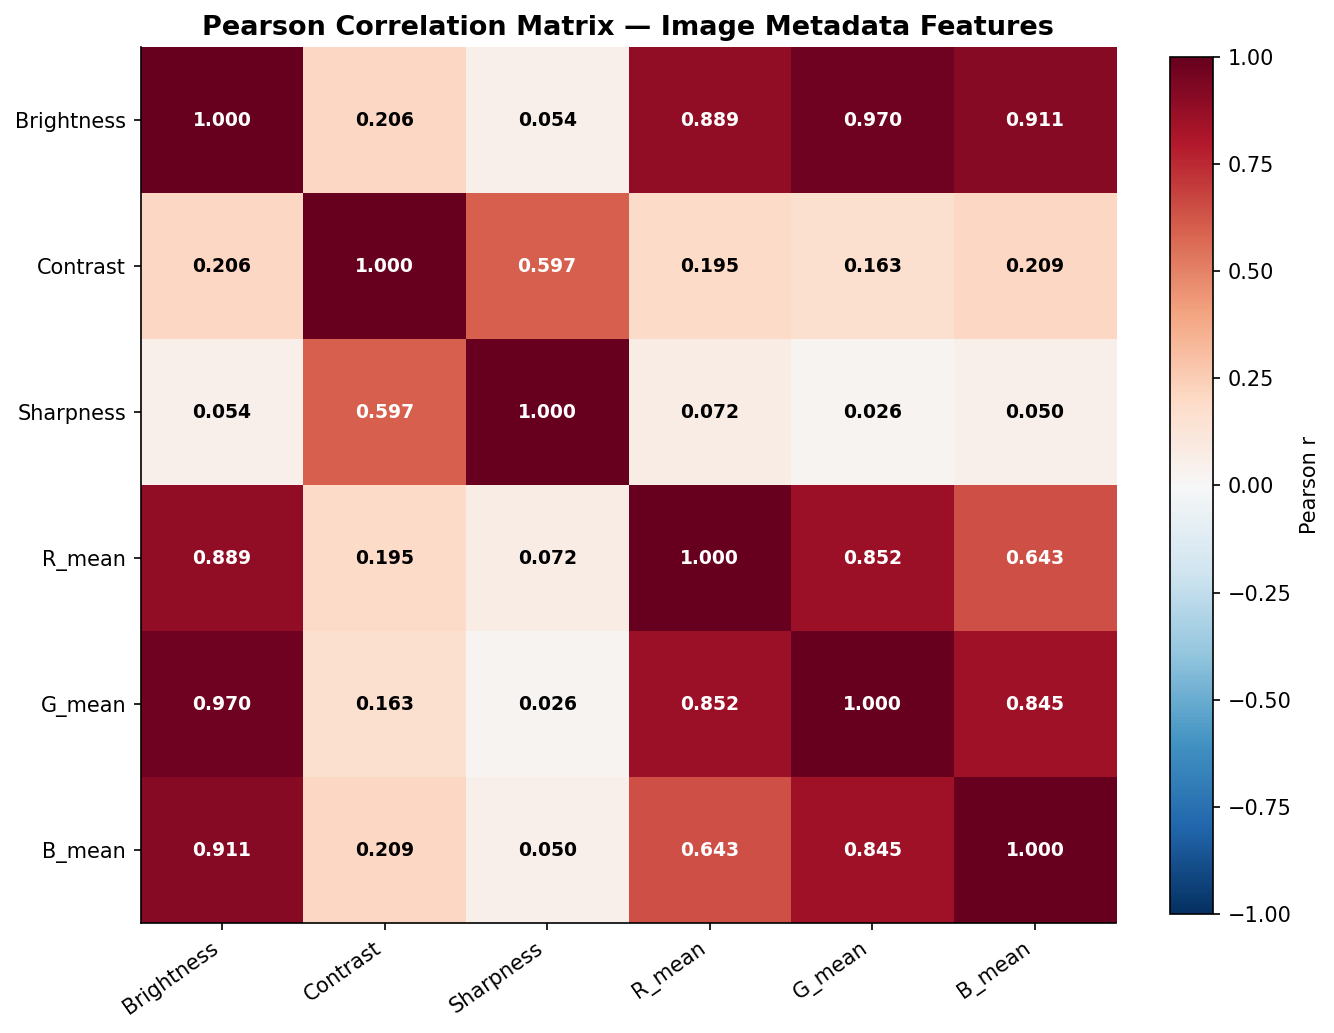
\includegraphics[width=0.60\textwidth]{figures/stat03_correlation_matrix.png}
\caption{Pearson correlation matrix between R, G, and B channel mean pixel values (per image). Strong inter-channel correlations reflect the dominance of luminance variation over chrominance variation.}
\label{fig:stat_corr_matrix}
\end{figure}

\begin{figure}[H]
\centering
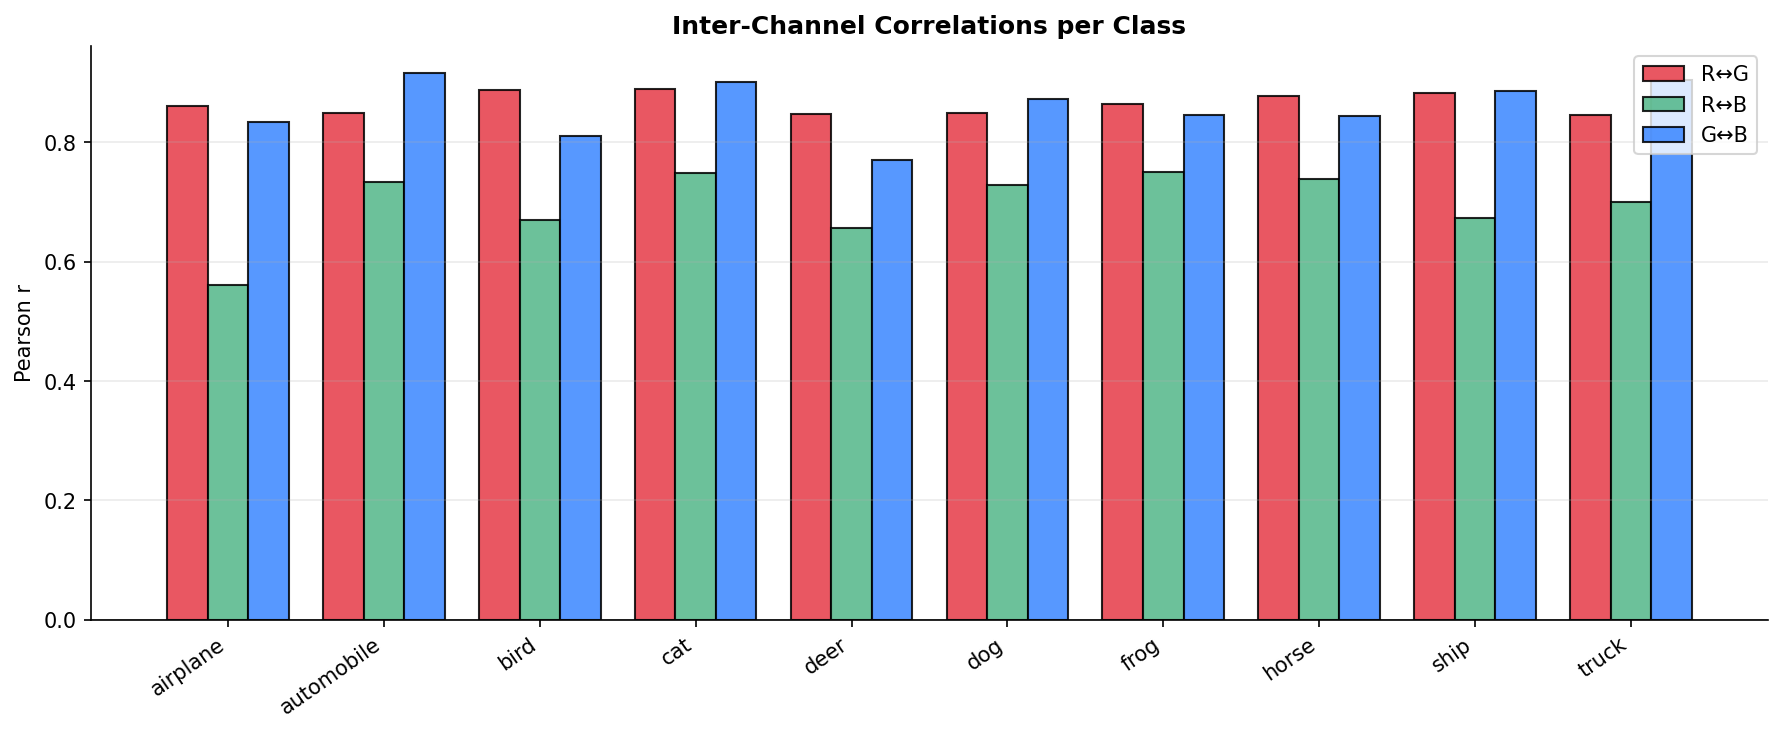
\includegraphics[width=0.85\textwidth]{figures/stat03_perclass_channel_corr.png}
\caption{Per-class channel correlation analysis. Some classes (e.g., ``frog'') show weaker R-B correlation due to their distinctive green-dominant colorspace.}
\label{fig:stat_perclass_corr}
\end{figure}

\subsubsection{Spatial Autocorrelation}
Figure~\ref{fig:stat_autocorr} presents spatial autocorrelation analysis confirming that neighboring pixels are highly correlated---a key property that autoencoders exploit during reconstruction.

\begin{figure}[H]
\centering
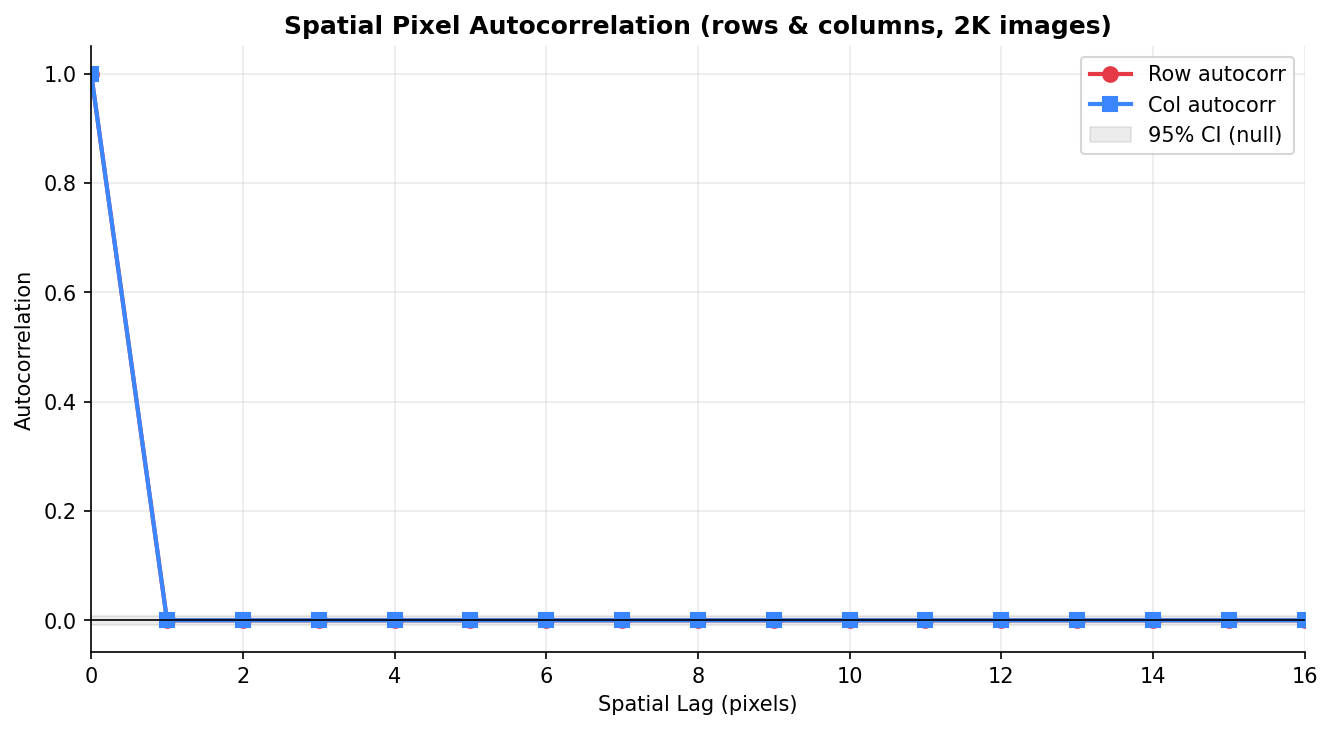
\includegraphics[width=0.80\textwidth]{figures/stat03_spatial_autocorr.png}
\caption{Spatial autocorrelation analysis. Strong positive correlation between adjacent pixels decays with distance, consistent with the smooth structure of natural images.}
\label{fig:stat_autocorr}
\end{figure}

\subsubsection{Channel Scatter Matrix}
Figure~\ref{fig:stat_scatter} shows the full scatter matrix of R, G, and B channel means, with per-class coloring. The ellipsoidal point clouds indicate approximate joint normality at the image level.

\begin{figure}[H]
\centering
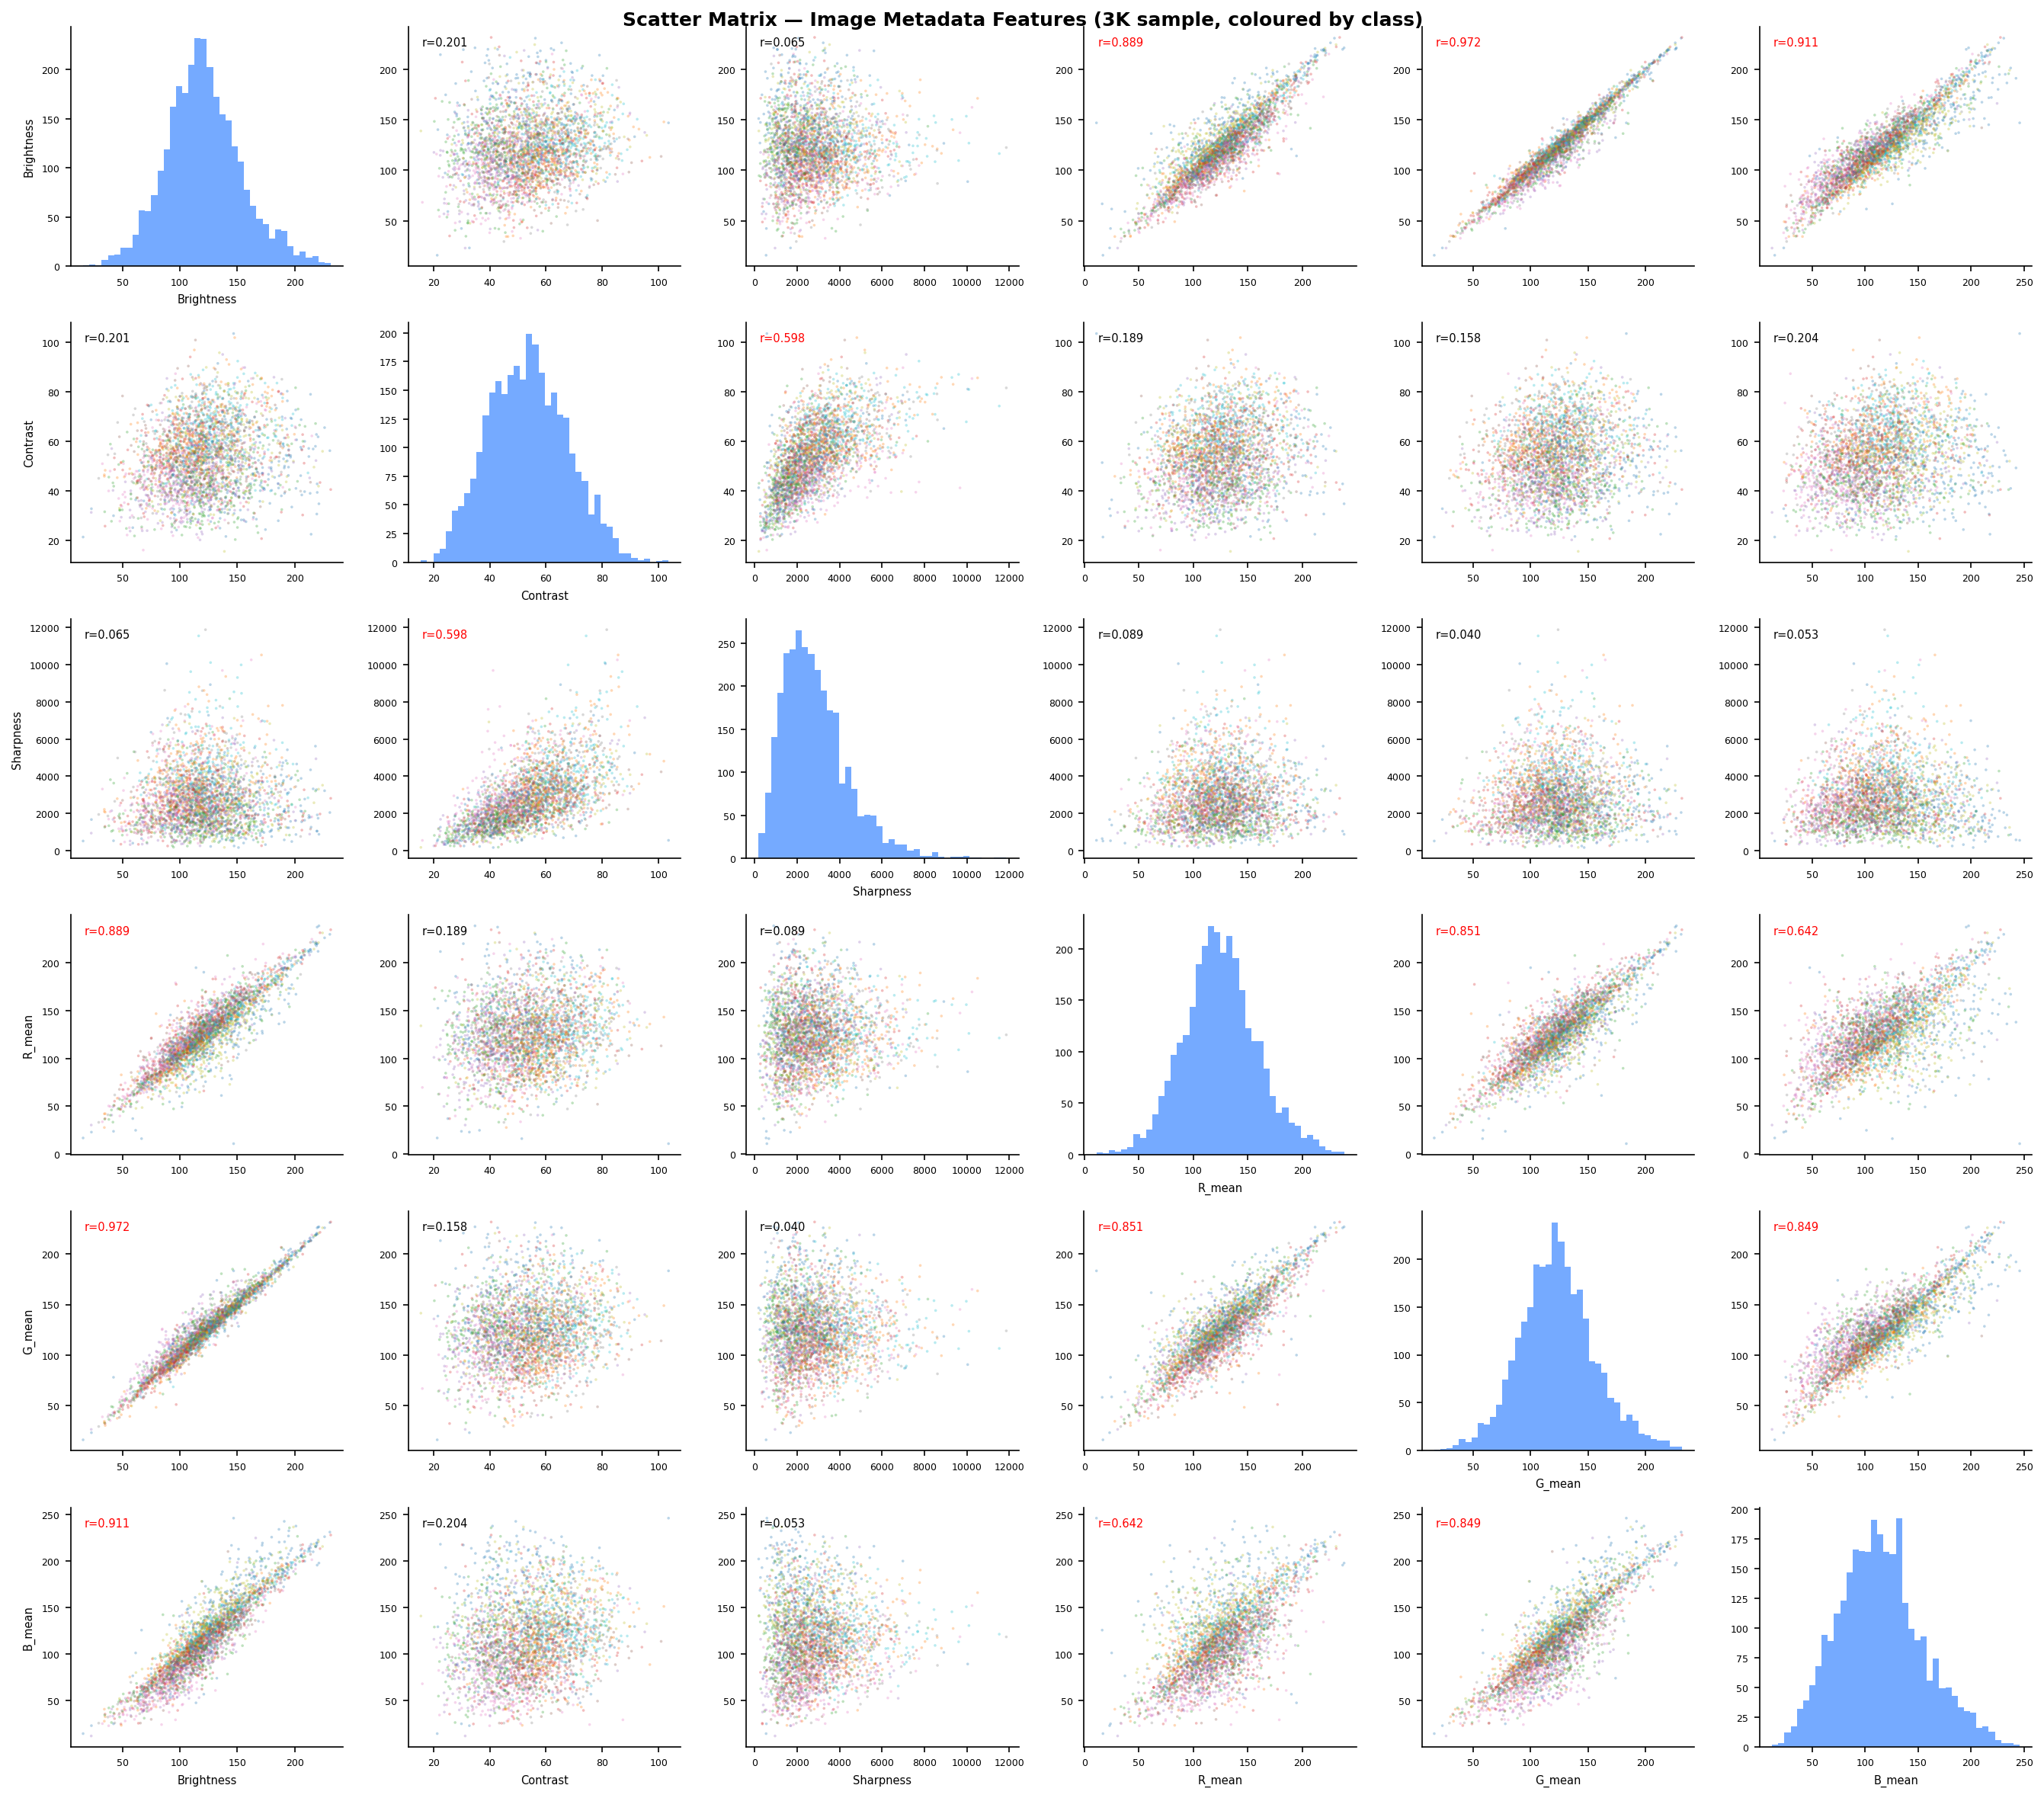
\includegraphics[width=0.75\textwidth]{figures/stat03_scatter_matrix.png}
\caption{R-G-B channel scatter matrix colored by CIFAR-10 class. Each point represents one training image. Class clusters are partially separable in the RGB feature space.}
\label{fig:stat_scatter}
\end{figure}


\subsection{Dimensionality Reduction}

\subsubsection{PCA Analysis}
Principal Component Analysis (PCA) was applied to reduce the 3{,}072-dimensional pixel space. Figure~\ref{fig:stat_pca_var} shows the cumulative explained variance, Figure~\ref{fig:stat_pca_2d} shows the 2D PCA projection, and Figure~\ref{fig:stat_eigenimages} displays the first eigenimages.

\begin{figure}[H]
\centering
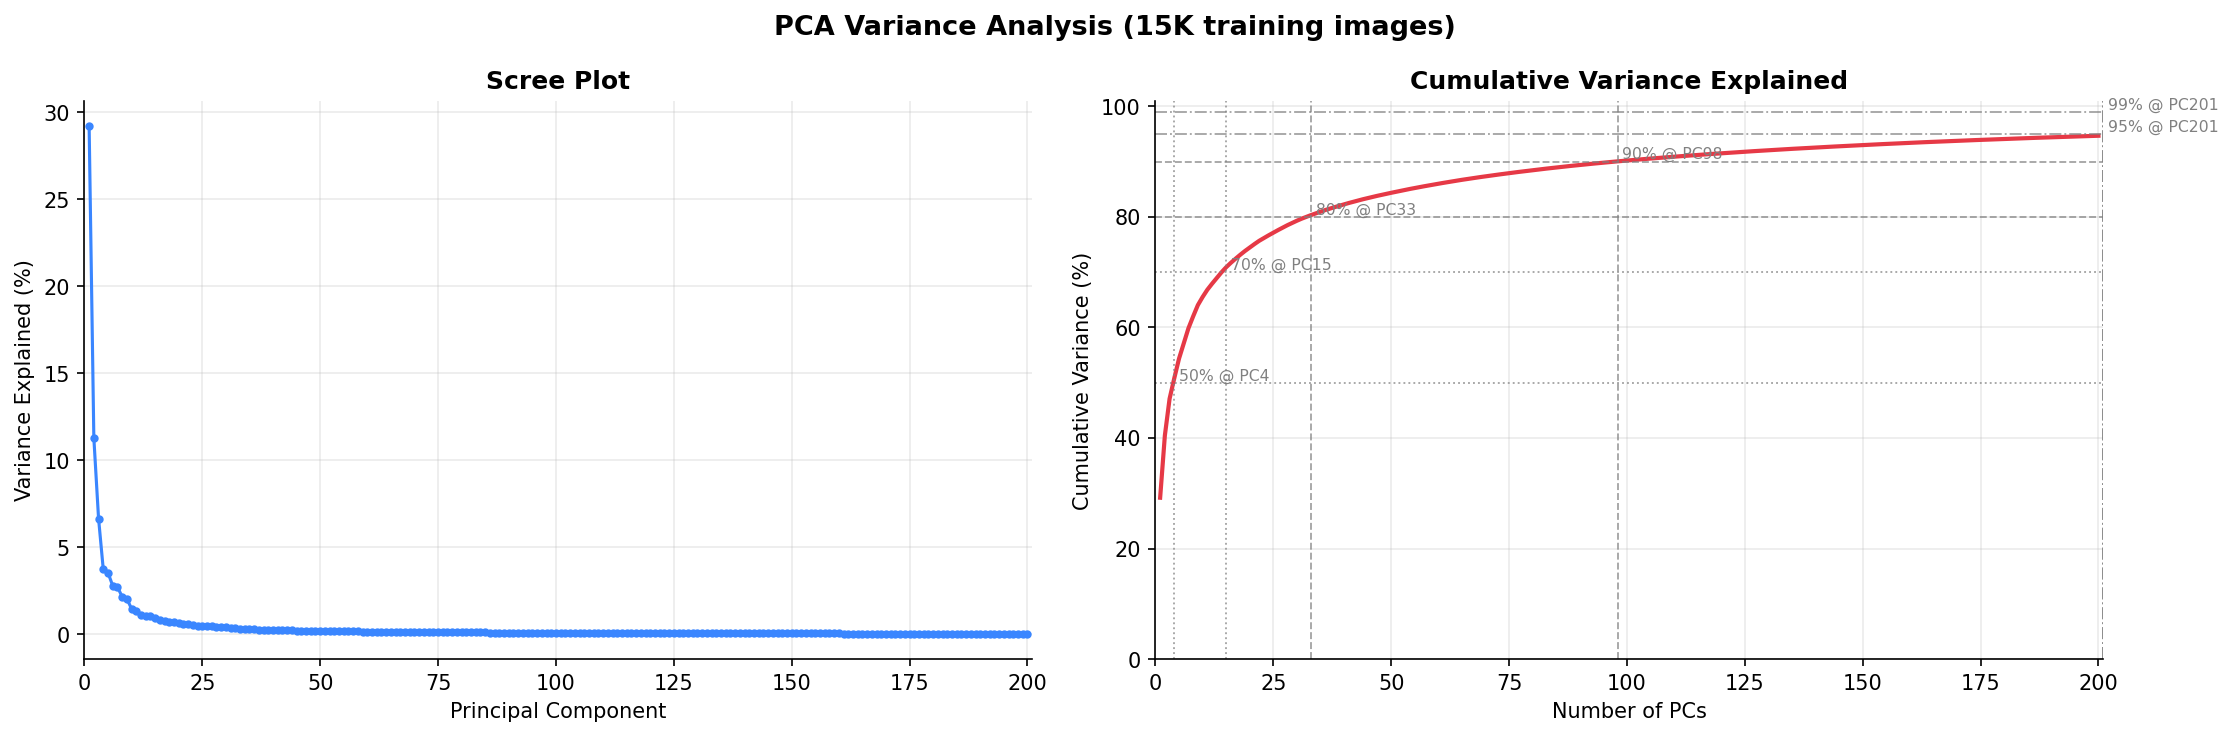
\includegraphics[width=0.75\textwidth]{figures/stat05_pca_variance.png}
\caption{PCA explained variance ratio. The first 100 components capture approximately 90\% of the total variance, demonstrating that CIFAR-10 images reside on a much lower-dimensional manifold.}
\label{fig:stat_pca_var}
\end{figure}

\begin{figure}[H]
\centering
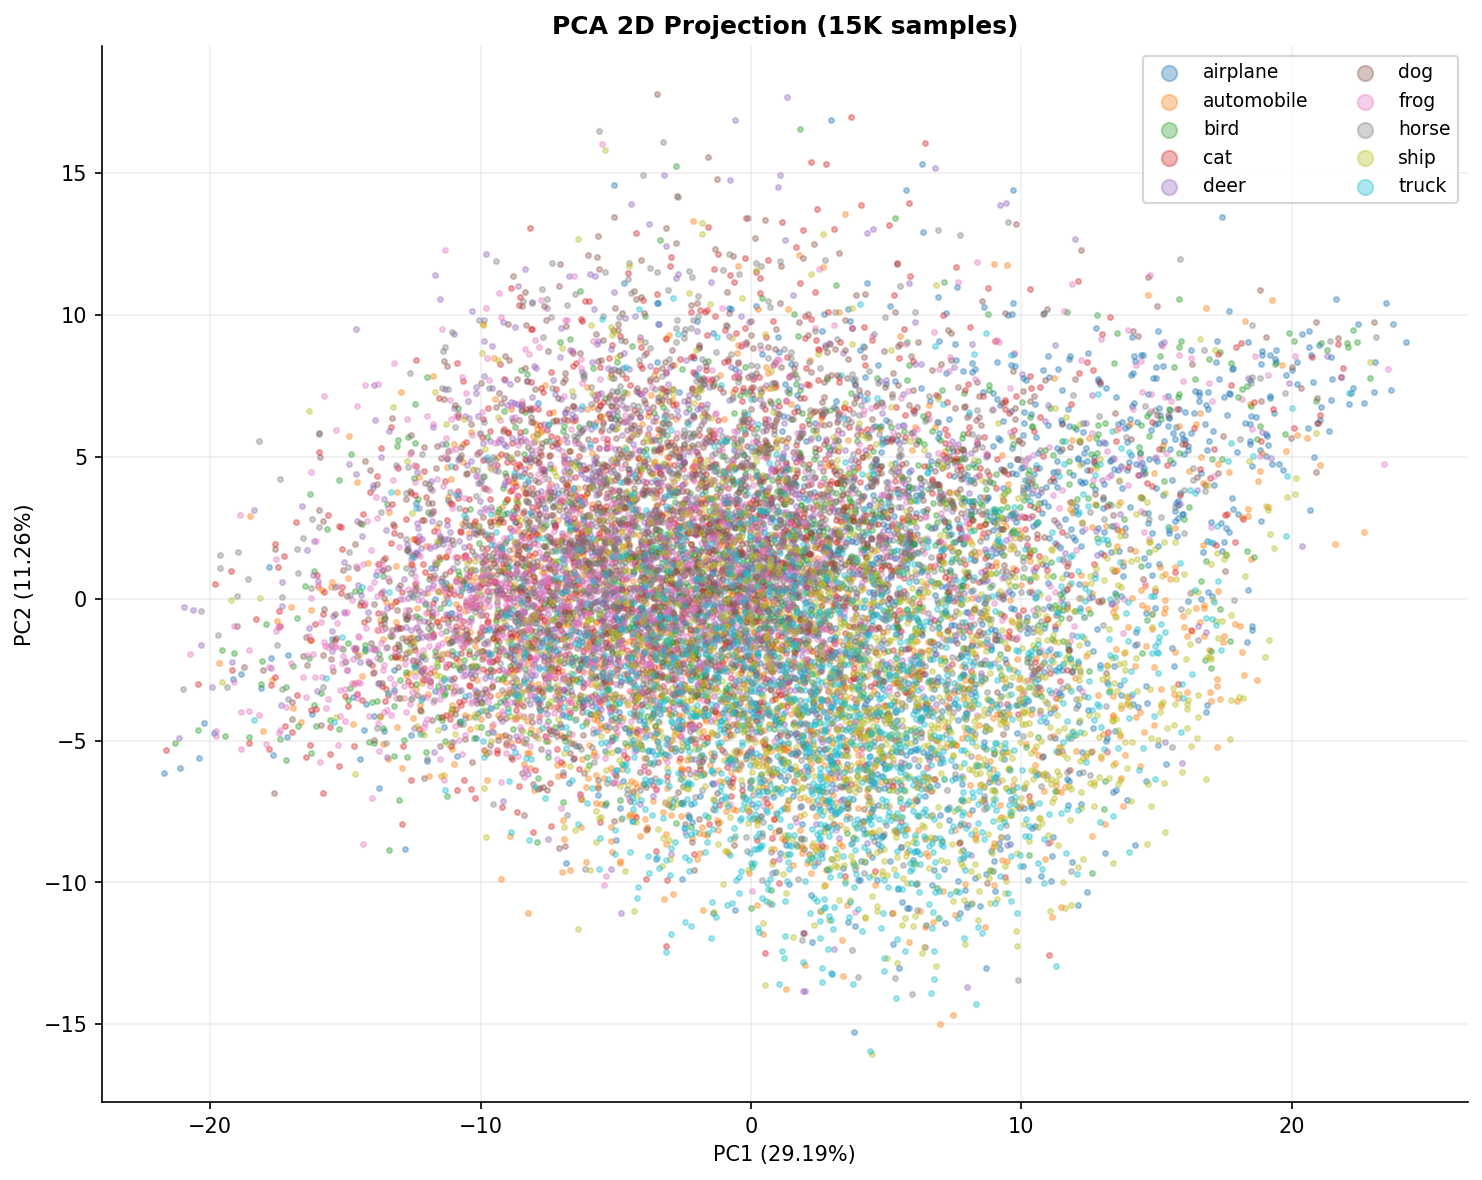
\includegraphics[width=0.80\textwidth]{figures/stat05_pca_2d.png}
\caption{2D PCA projection of CIFAR-10 training images colored by class. While significant overlap exists (expected for 3{,}072$\to$2 compression), some classes form partially separable clusters.}
\label{fig:stat_pca_2d}
\end{figure}

\begin{figure}[H]
\centering
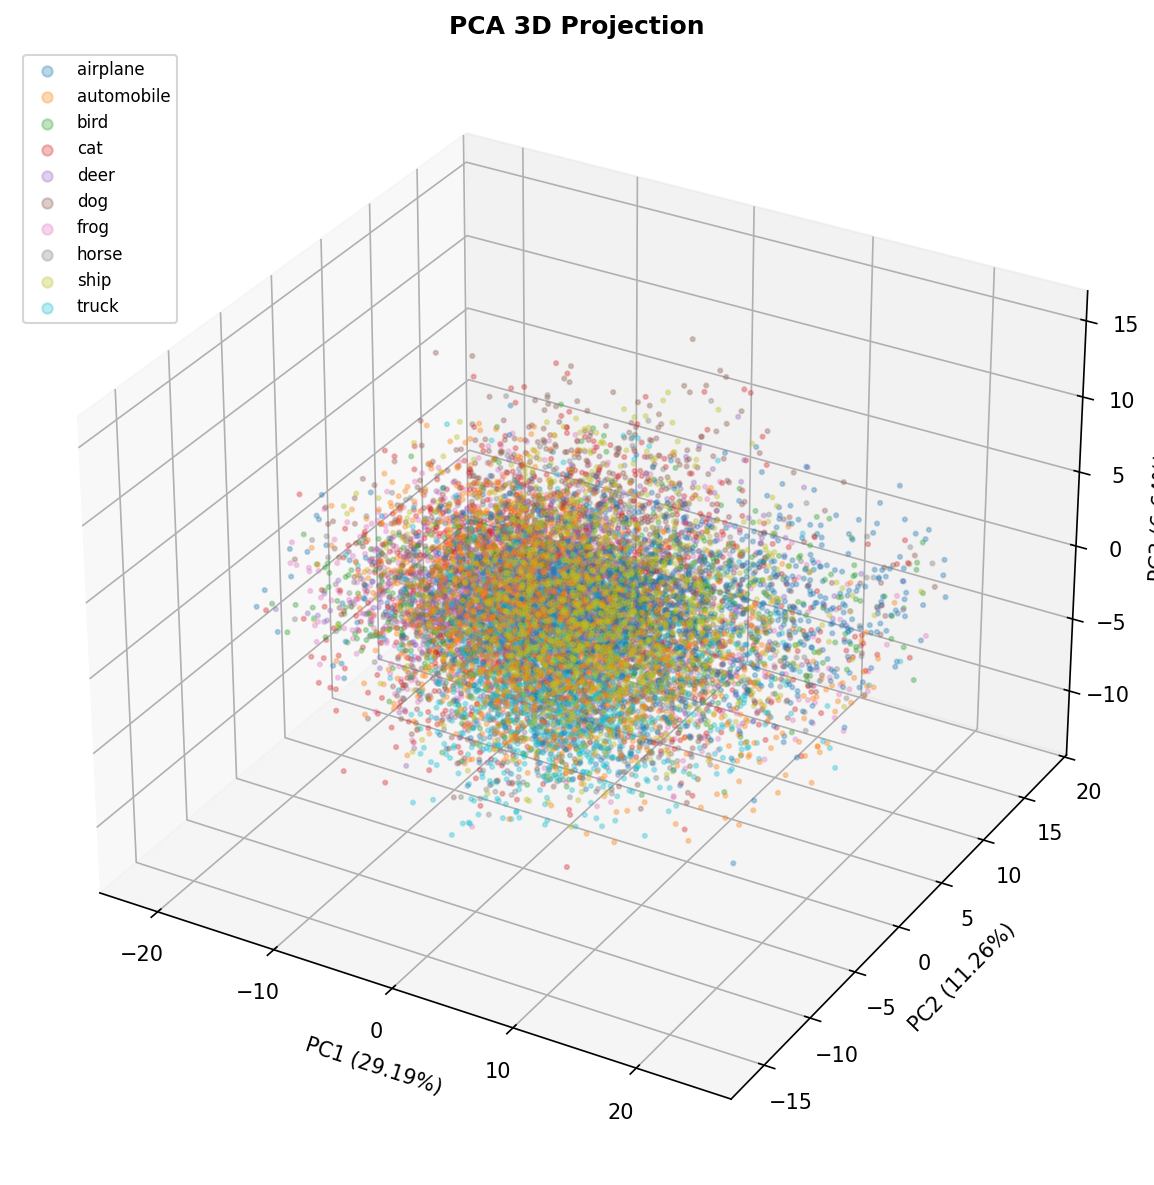
\includegraphics[width=0.80\textwidth]{figures/stat05_pca_3d.png}
\caption{3D PCA projection of CIFAR-10 training images. The third component adds minor separability for classes like ``frog'' (green-dominated) and ``ship'' (blue-dominated).}
\label{fig:stat_pca_3d}
\end{figure}

\begin{figure}[H]
\centering
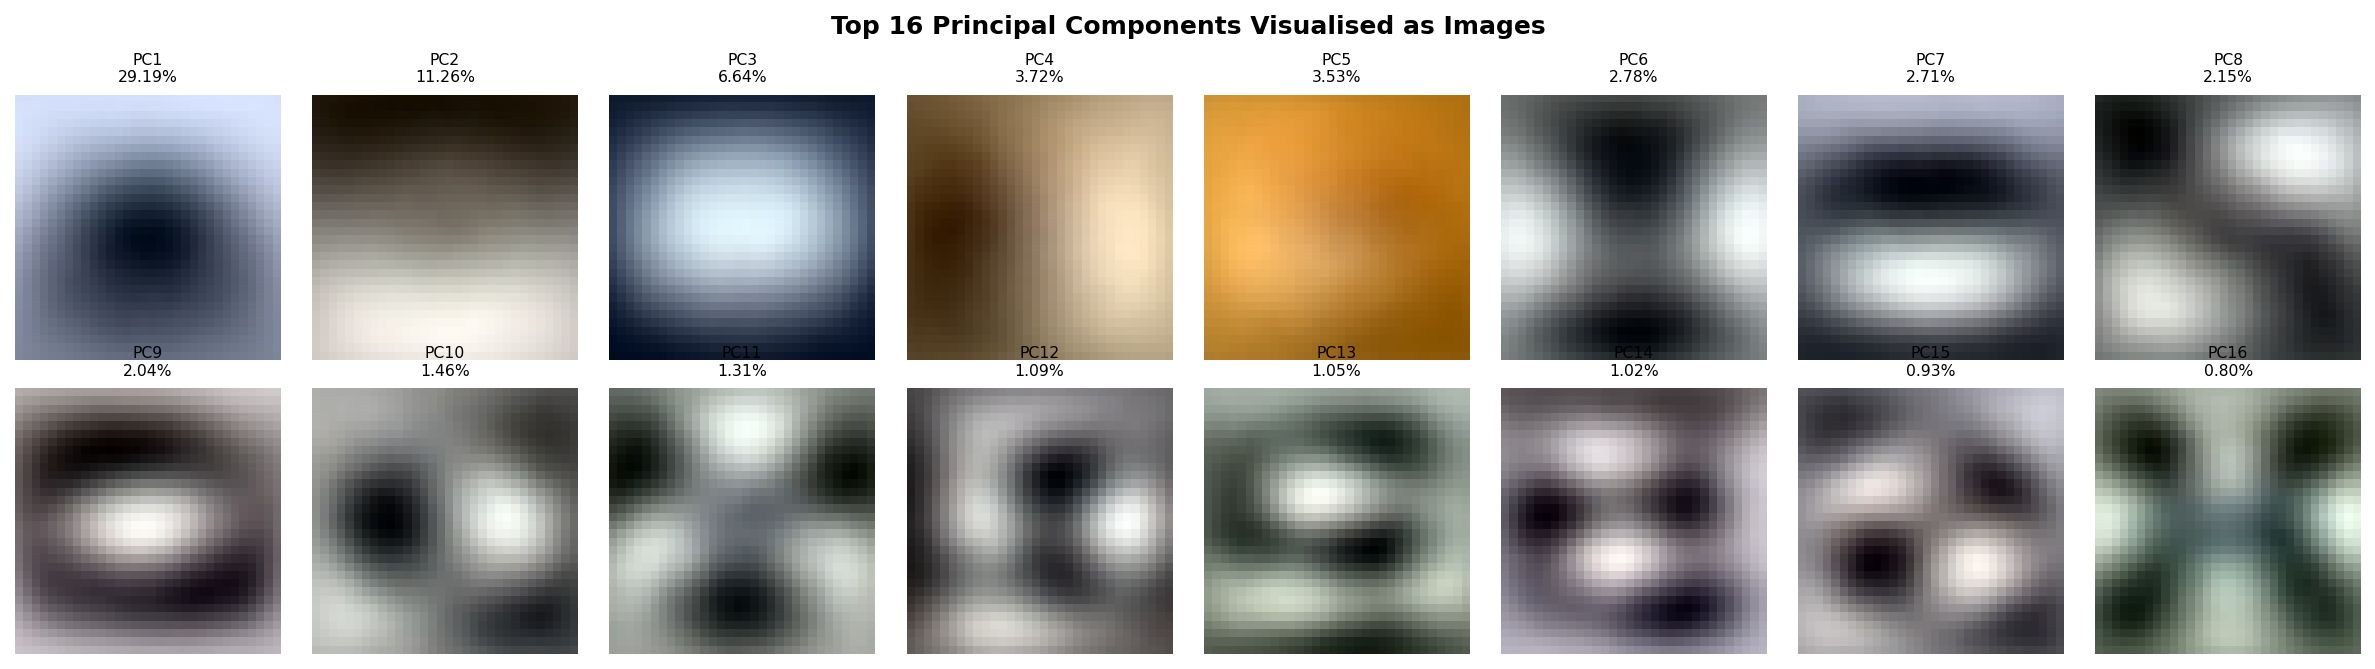
\includegraphics[width=0.85\textwidth]{figures/stat05_eigenimages.png}
\caption{Eigenimages (principal components) reshaped to 32$\times$32$\times$3. The first eigenimage captures overall brightness, while subsequent components capture increasingly fine-grained spatial patterns and color variations.}
\label{fig:stat_eigenimages}
\end{figure}

\subsubsection{t-SNE Visualization}
Figure~\ref{fig:stat_tsne} shows the t-SNE embedding. Classes with more distinctive visual features (vehicles vs.\ animals) form more coherent clusters than visually similar classes (cat vs.\ dog).

\begin{figure}[H]
\centering
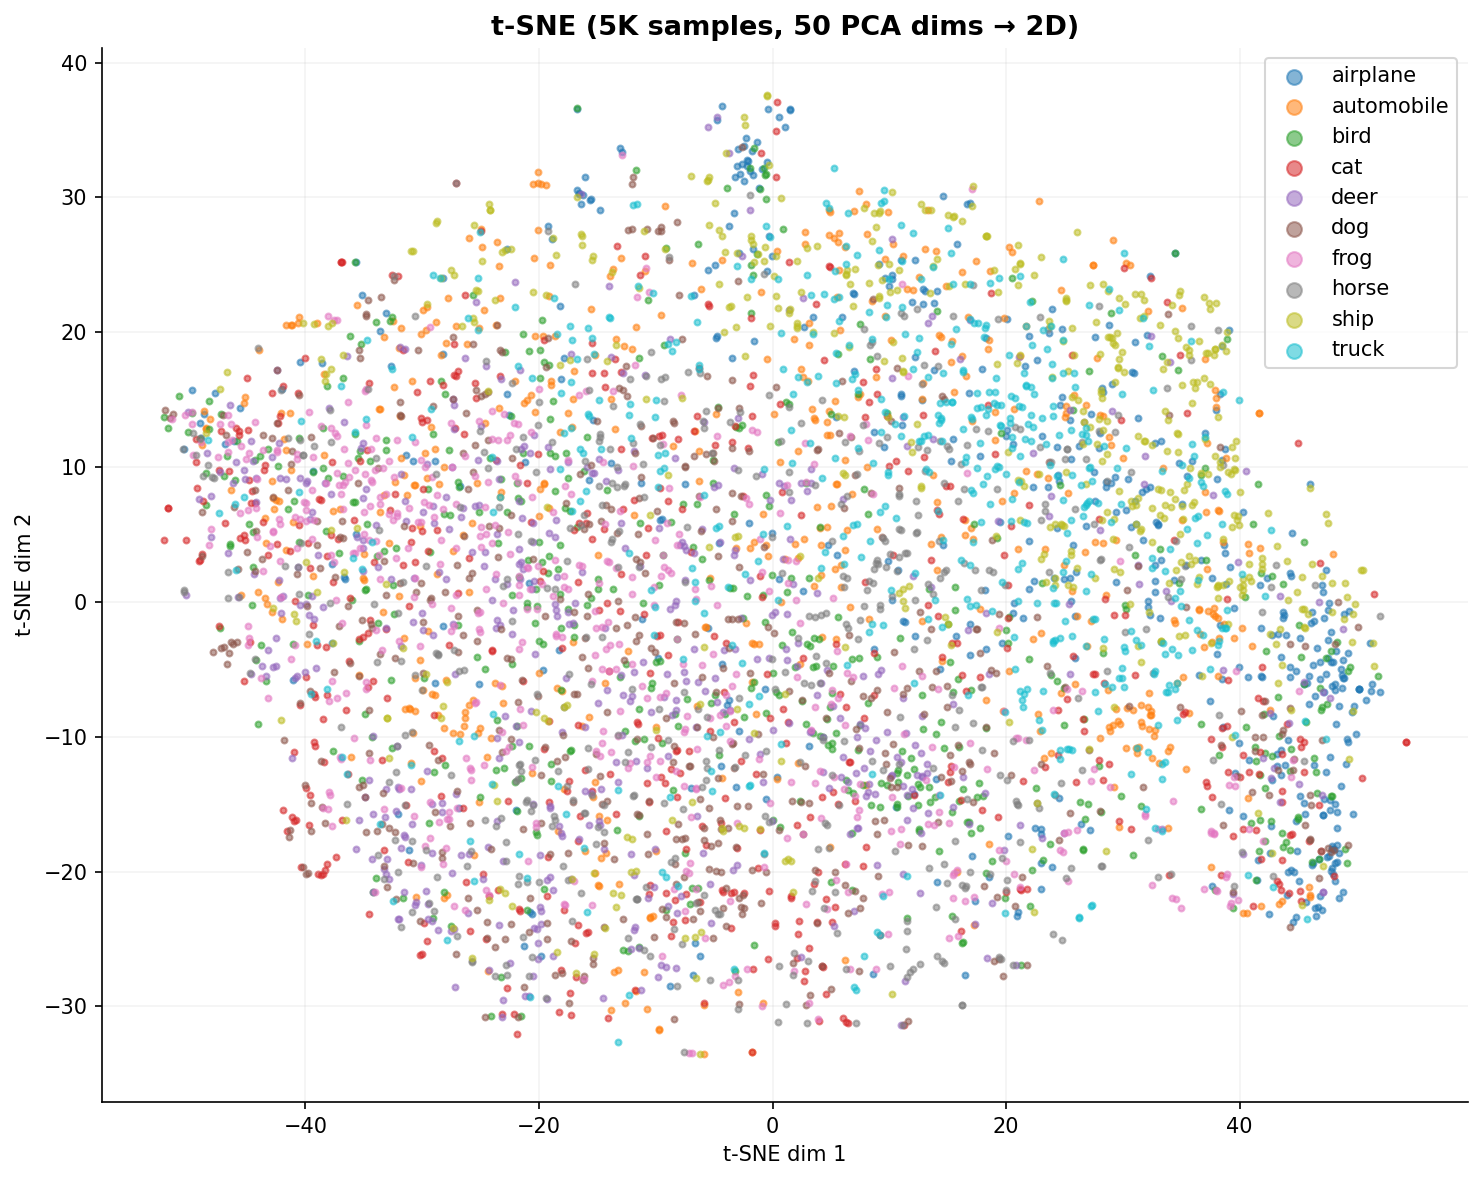
\includegraphics[width=0.80\textwidth]{figures/stat05_tsne.png}
\caption{t-SNE 2D embedding of CIFAR-10 training images. Non-linear dimensionality reduction reveals tighter class clusters than PCA, particularly for structured categories like ``ship'' and ``automobile.'' Visually similar categories like ``cat'' and ``dog'' remain heavily mixed.}
\label{fig:stat_tsne}
\end{figure}


\subsection{Class Balance and Image Quality}

\begin{figure}[H]
\centering
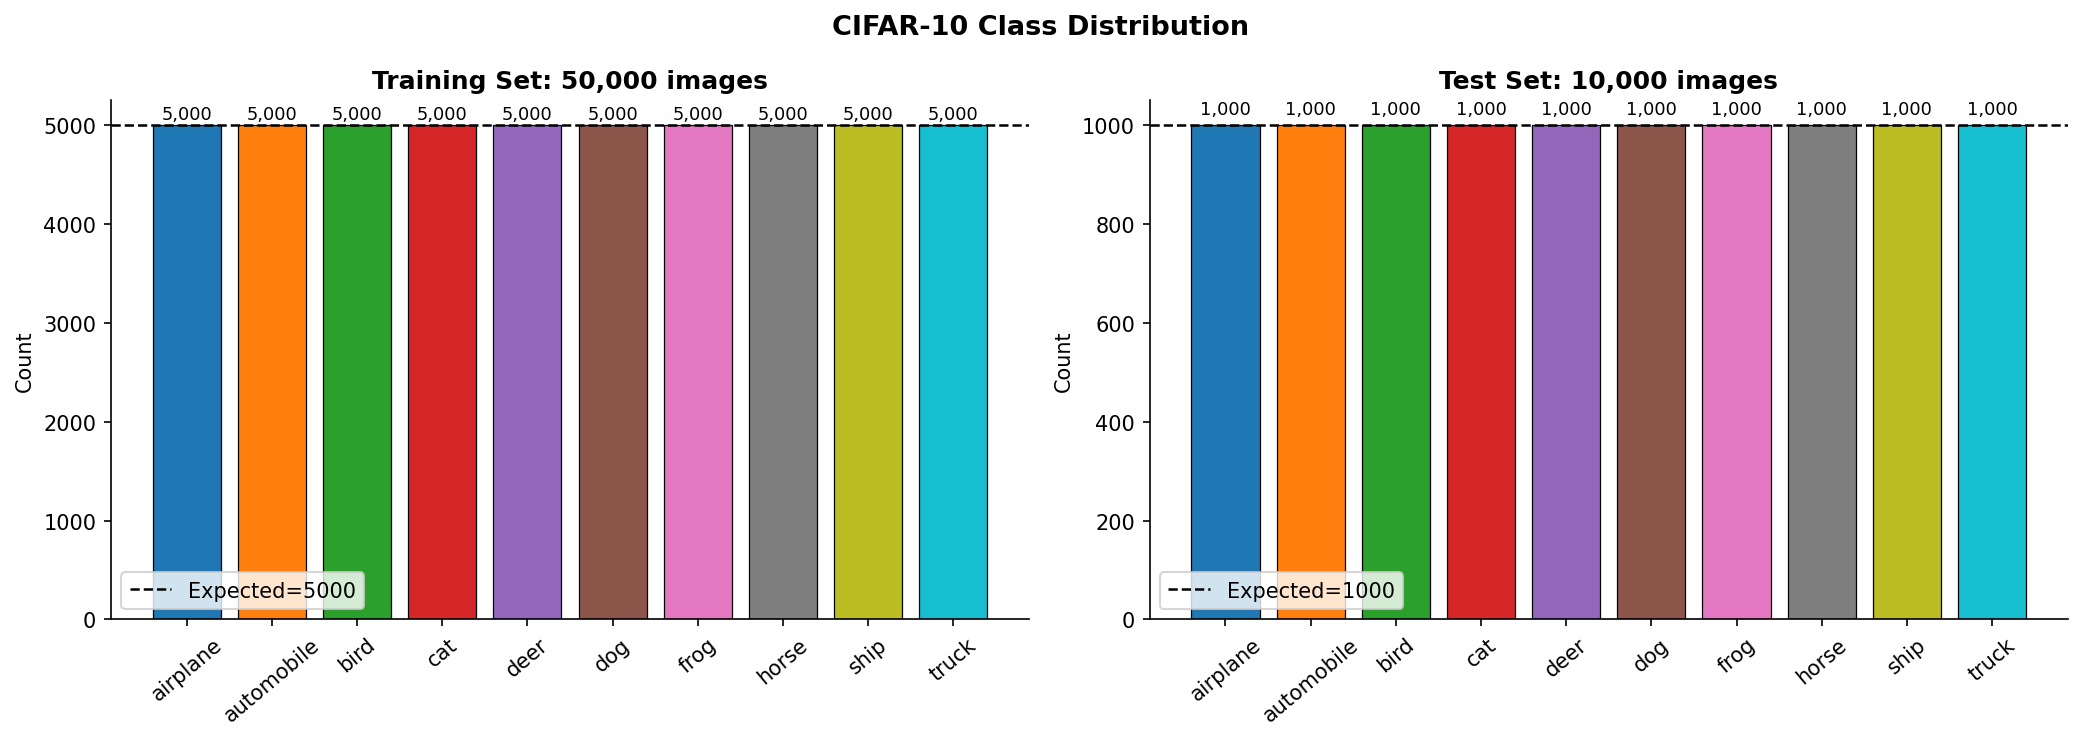
\includegraphics[width=0.80\textwidth]{figures/stat04_class_distribution.png}
\caption{Detailed class distribution analysis with per-class sample counts and proportions, confirming perfect balance across all 10 classes.}
\label{fig:stat_class_detail}
\end{figure}

\begin{figure}[H]
\centering
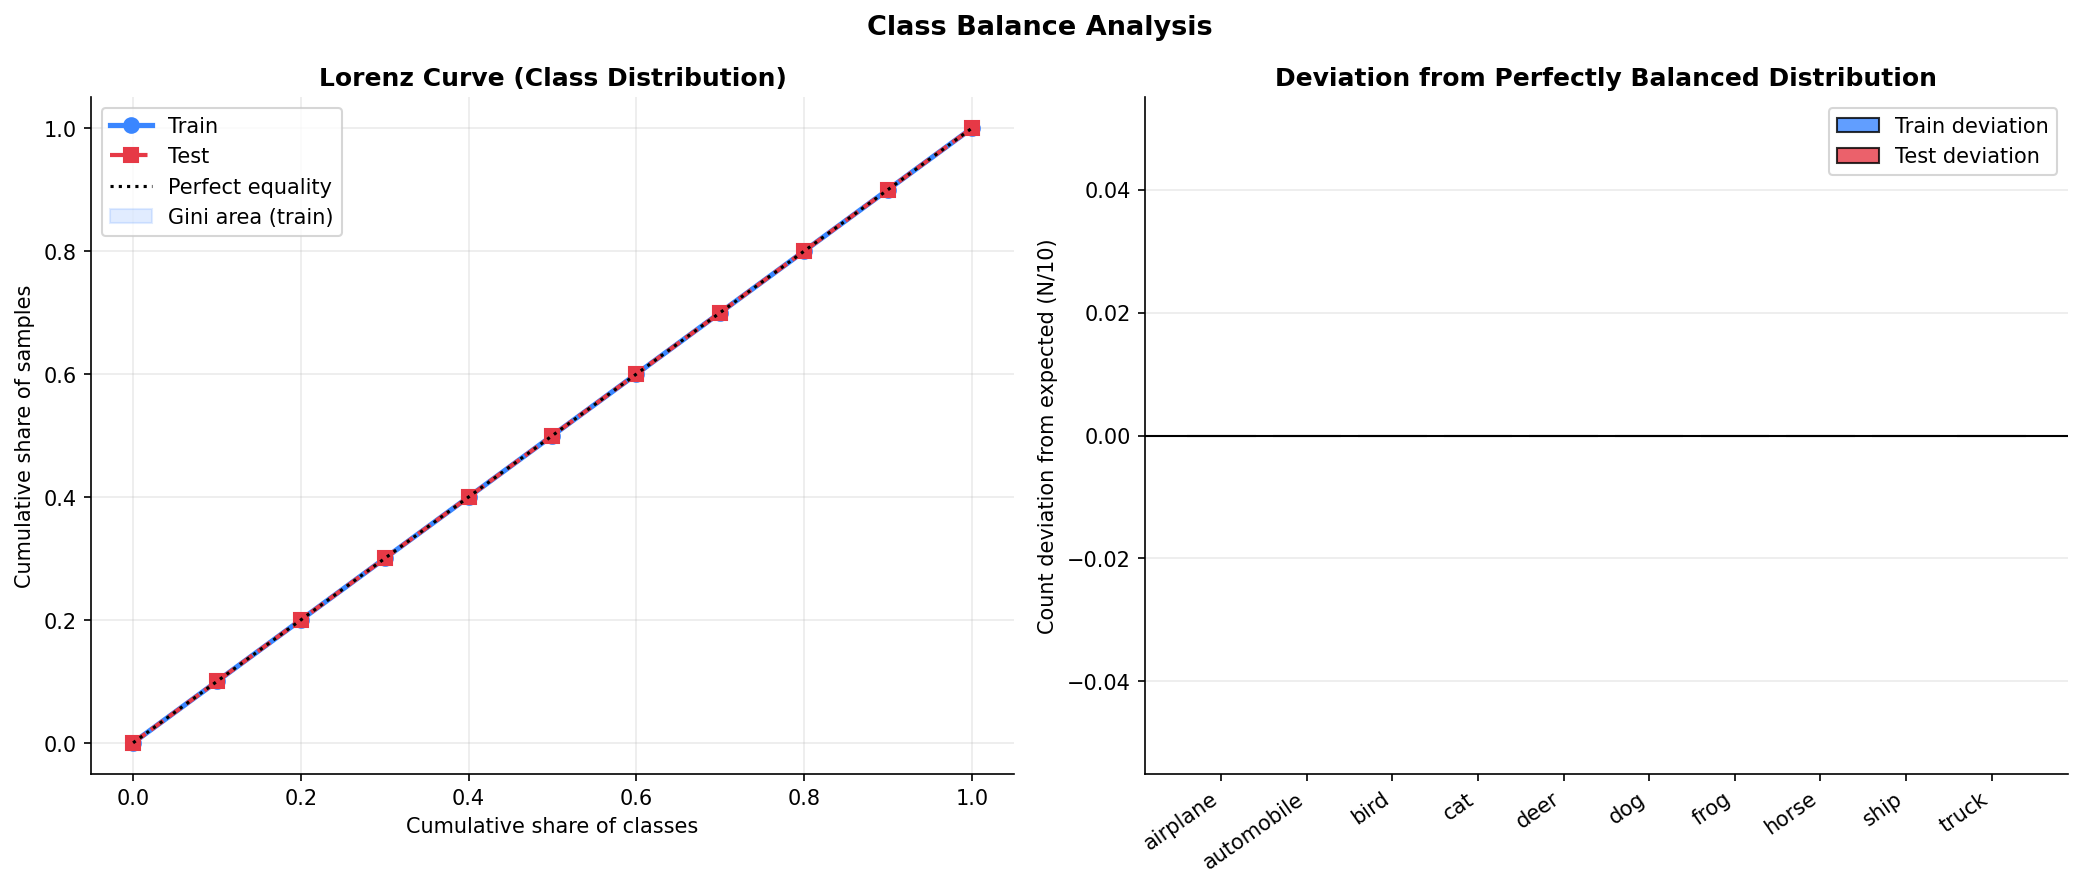
\includegraphics[width=0.80\textwidth]{figures/stat04_class_balance.png}
\caption{Class balance verification showing uniform representation across train/test splits.}
\label{fig:stat_class_balance}
\end{figure}

\begin{figure}[H]
\centering
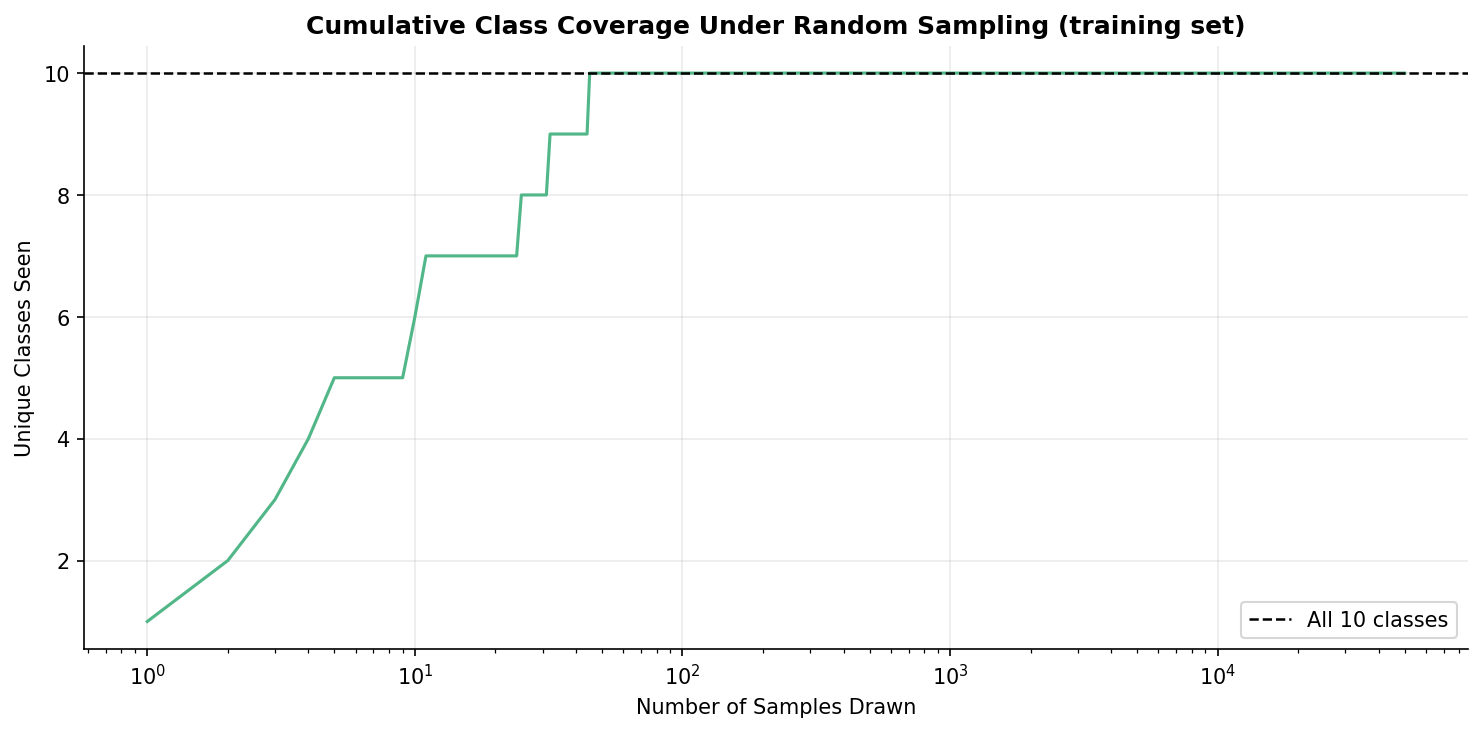
\includegraphics[width=0.75\textwidth]{figures/stat04_cumulative_coverage.png}
\caption{Cumulative class coverage: the contribution of each class to the total dataset, illustrating perfect balance.}
\label{fig:stat_cumulative}
\end{figure}

\begin{figure}[H]
\centering
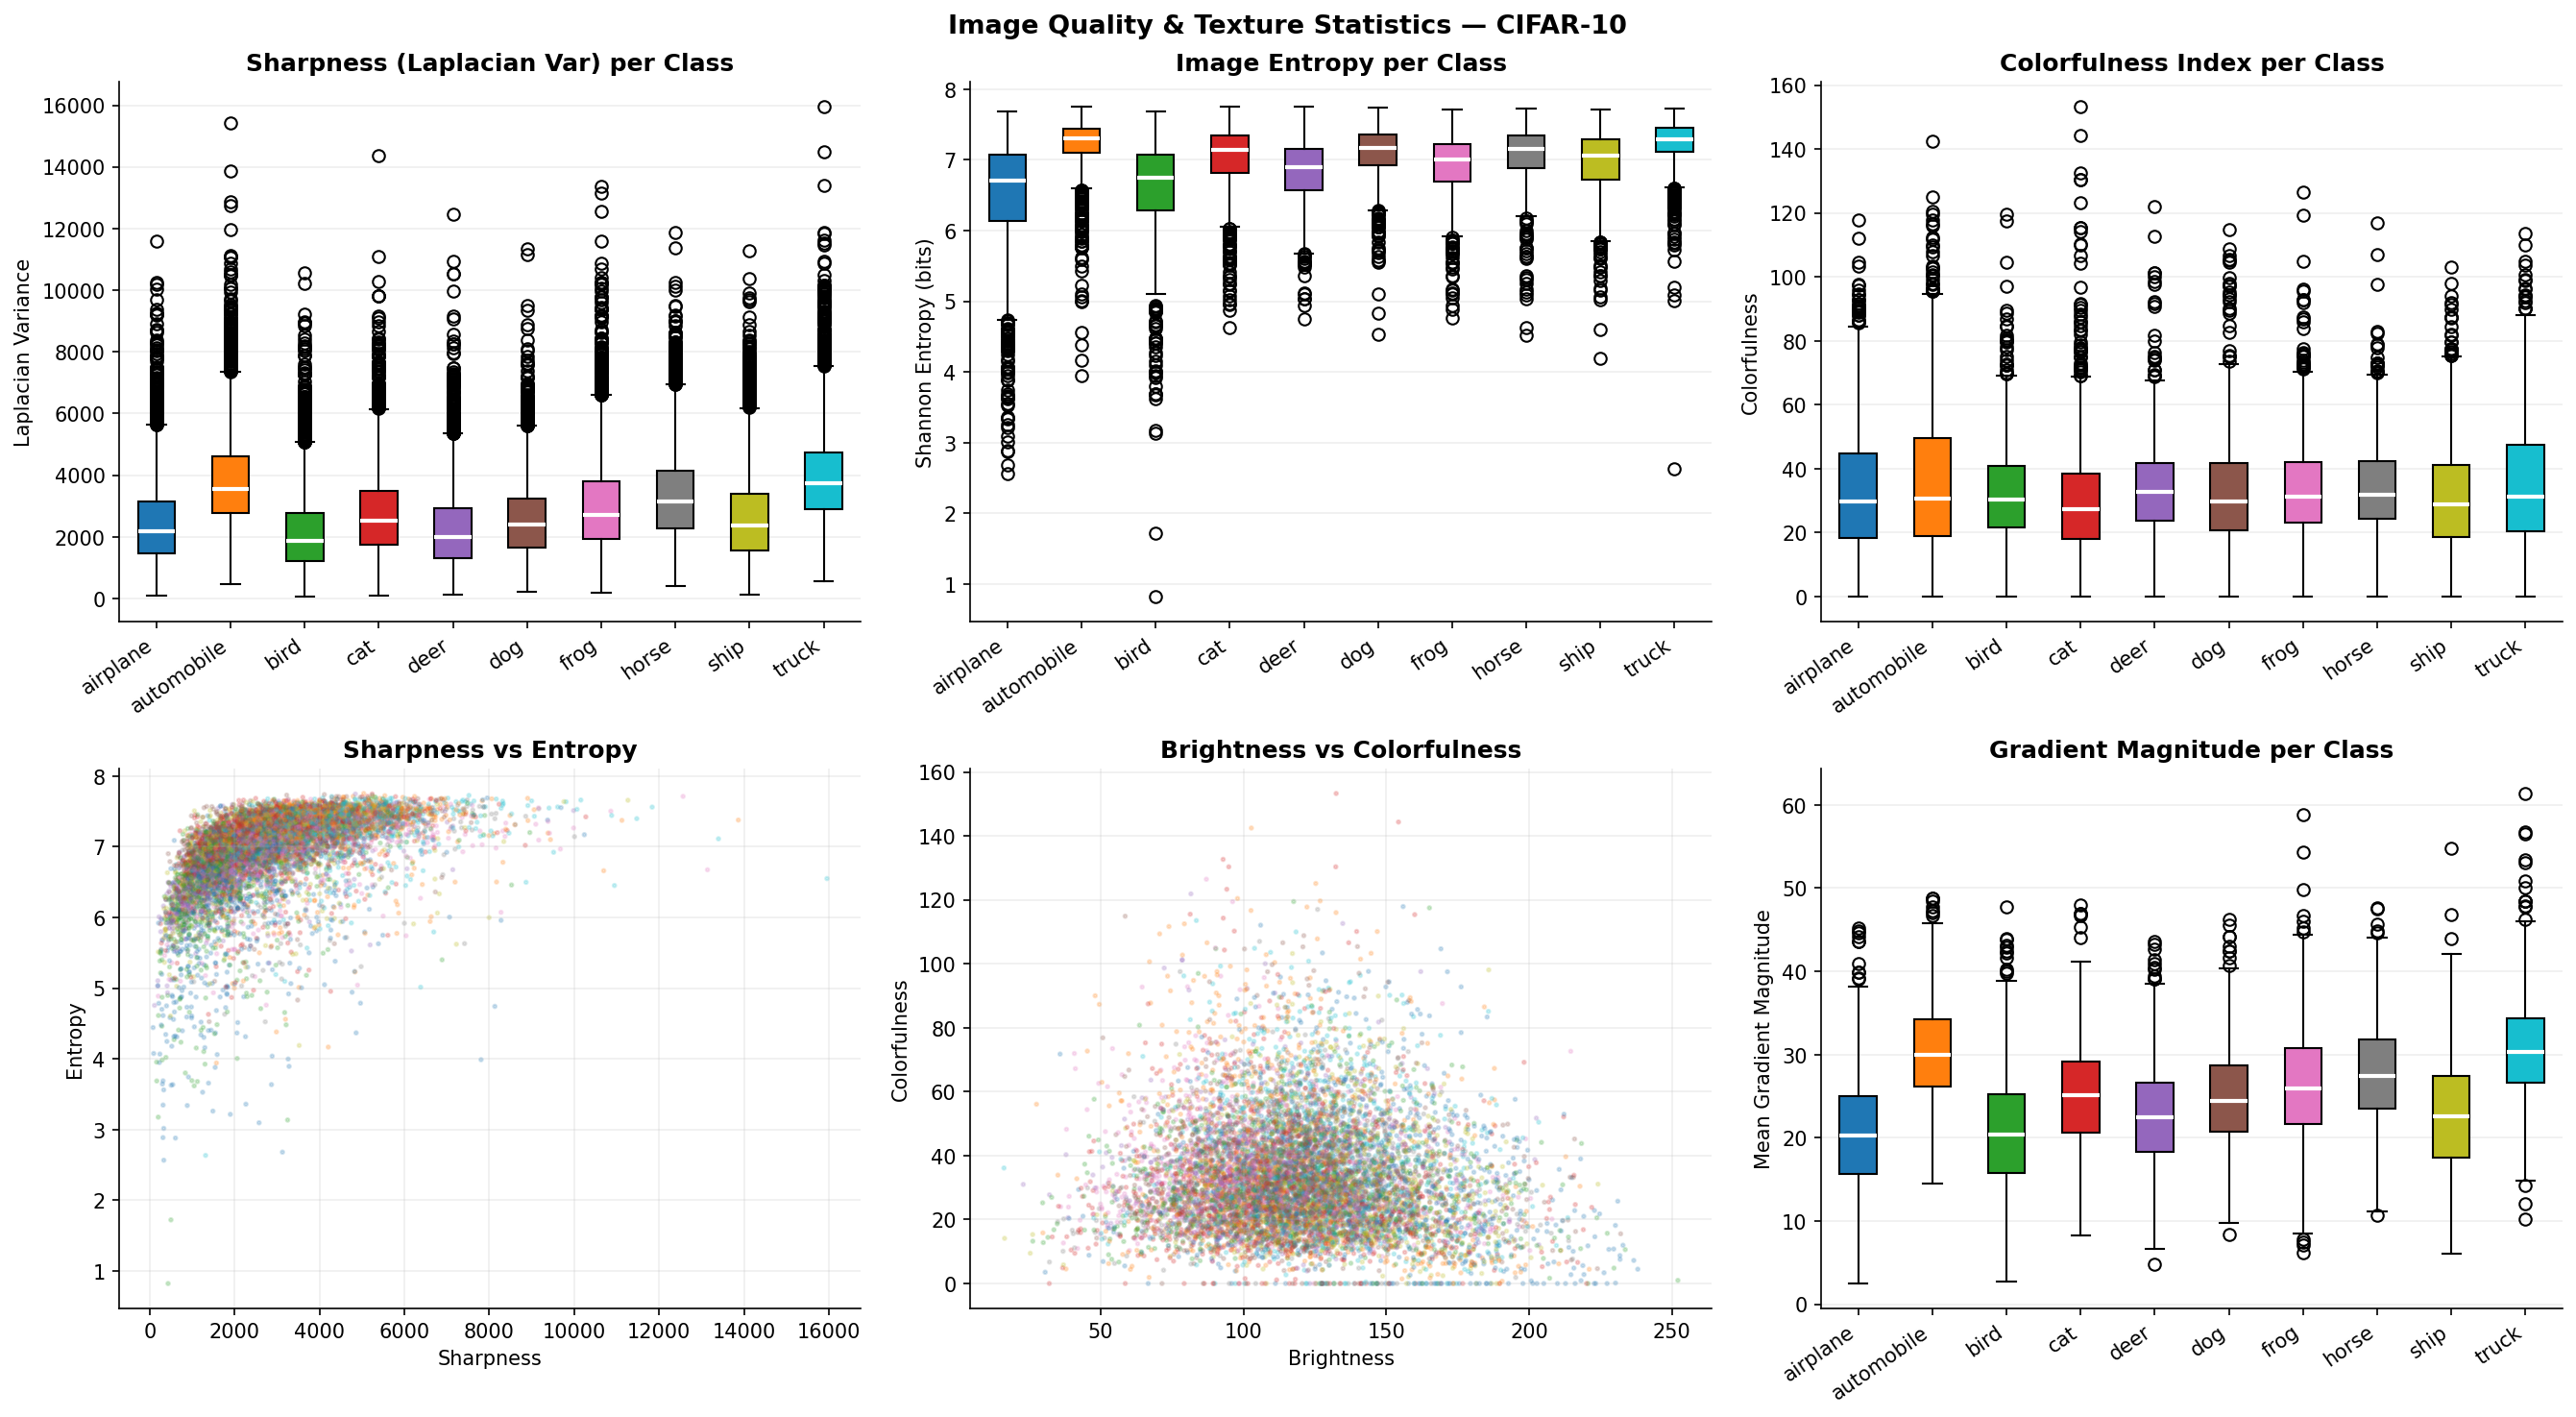
\includegraphics[width=0.90\textwidth]{figures/stat06_image_quality.png}
\caption{Image quality assessment metrics computed across the CIFAR-10 dataset, including entropy, Laplacian variance (sharpness), and dynamic range per class.}
\label{fig:stat_quality}
\end{figure}


% ─────────────────────────────────────────────────────────────────────────
% 4. NOISE INJECTION
% ─────────────────────────────────────────────────────────────────────────
\section{Noise Injection}
\label{sec:noise}

Two types of noise are applied to corrupt the clean images during training and evaluation.

\subsection{Gaussian Noise}
Additive white Gaussian noise (AWGN) with zero mean and standard deviation $\sigma$ is added to each pixel independently:
\begin{equation}
    x_{\text{noisy}} = \text{clip}\!\left(x_{\text{clean}} + \mathcal{N}(0, \sigma^2),\, 0,\, 1\right)
\end{equation}
This models sensor noise in digital cameras and thermal noise in communication channels. Higher $\sigma$ values produce more severe corruption. The clipping ensures pixel values remain in $[0,1]$.

\subsection{Salt-and-Pepper Noise}
Salt-and-pepper (impulse) noise randomly sets a fraction $p$ of pixels to either the maximum value~1 (salt) or the minimum value~0 (pepper):
\begin{equation}
    x_{\text{noisy}}(i) =
    \begin{cases}
        1 & \text{with probability } p/2 \\
        0 & \text{with probability } p/2 \\
        x_{\text{clean}}(i) & \text{otherwise}
    \end{cases}
\end{equation}
This simulates dead/stuck pixels, bit errors during transmission, and analog-to-digital converter faults.

\subsection{Noise Visualization}
Figure~\ref{fig:noise_types} shows a side-by-side comparison of both noise types at different severity levels, and Figure~\ref{fig:noise_progression} shows the progressive degradation of image quality as noise levels increase.

\begin{figure}[H]
\centering
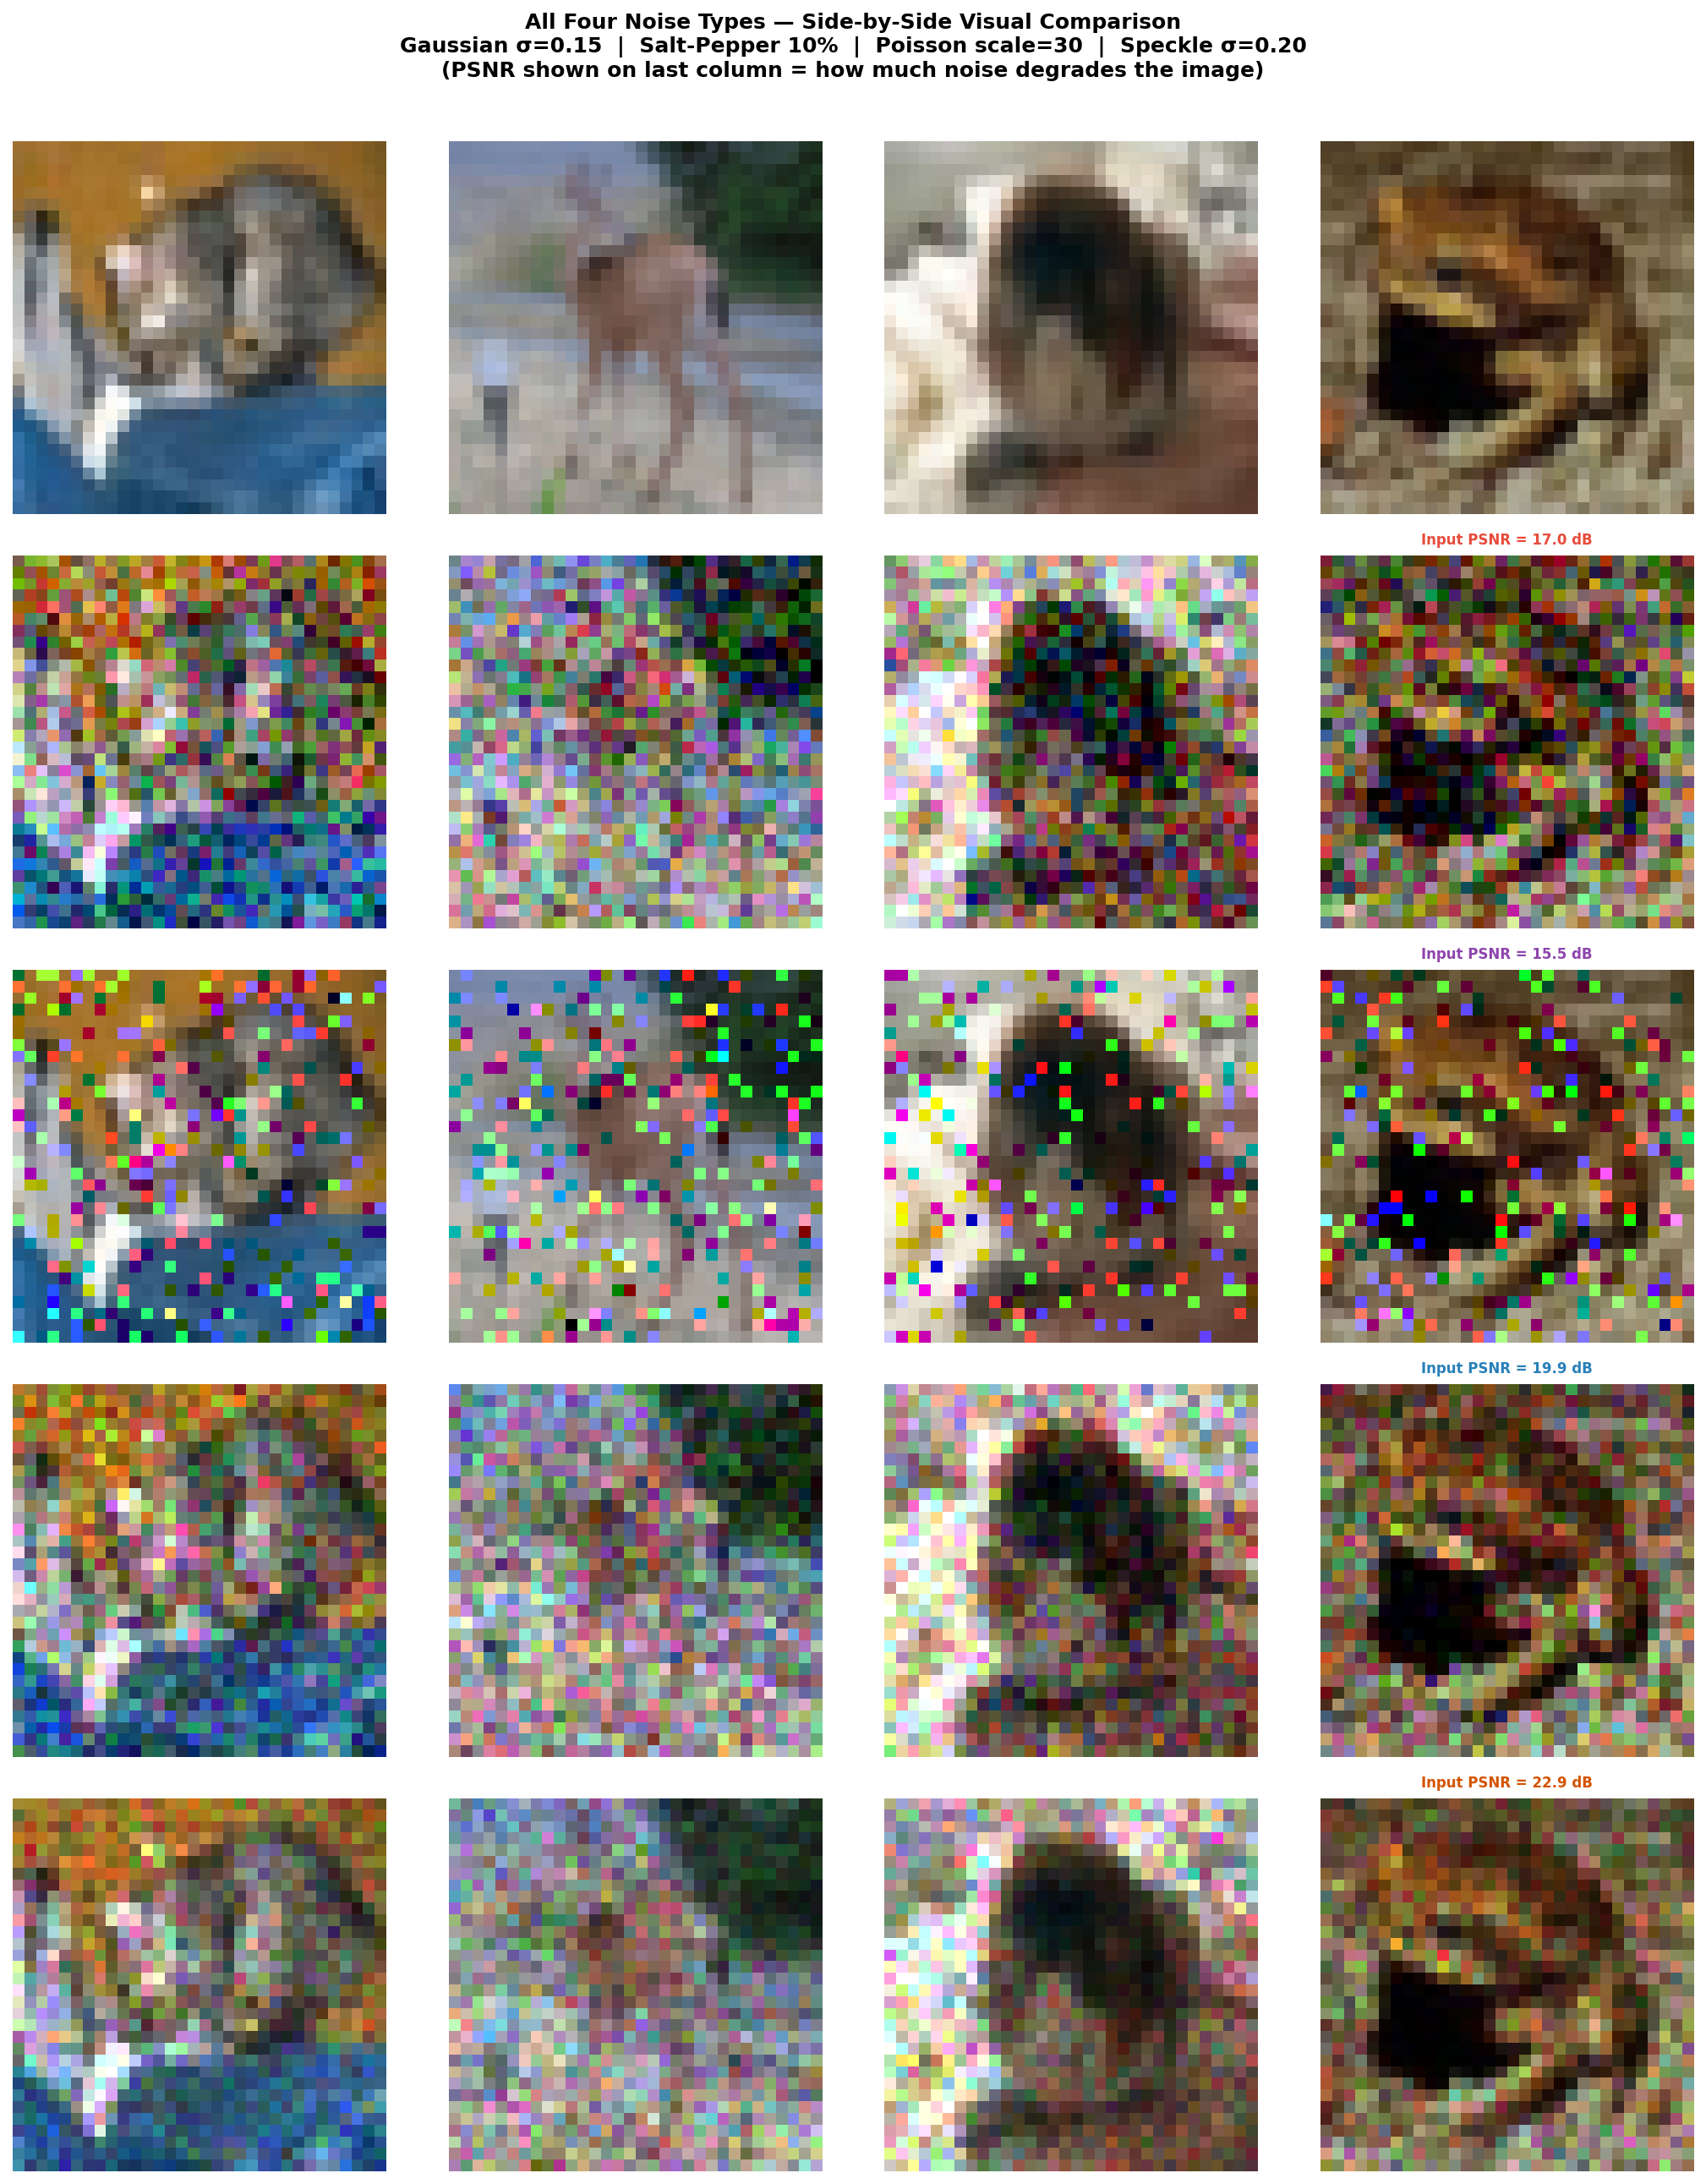
\includegraphics[width=0.90\textwidth]{figures/fig05_noise_types_comparison.png}
\caption{Comparison of Gaussian and Salt-and-Pepper noise at multiple severity levels. The Gaussian noise produces a uniform speckle pattern, while S\&P creates sparse extreme-value pixels.}
\label{fig:noise_types}
\end{figure}

\begin{figure}[H]
\centering
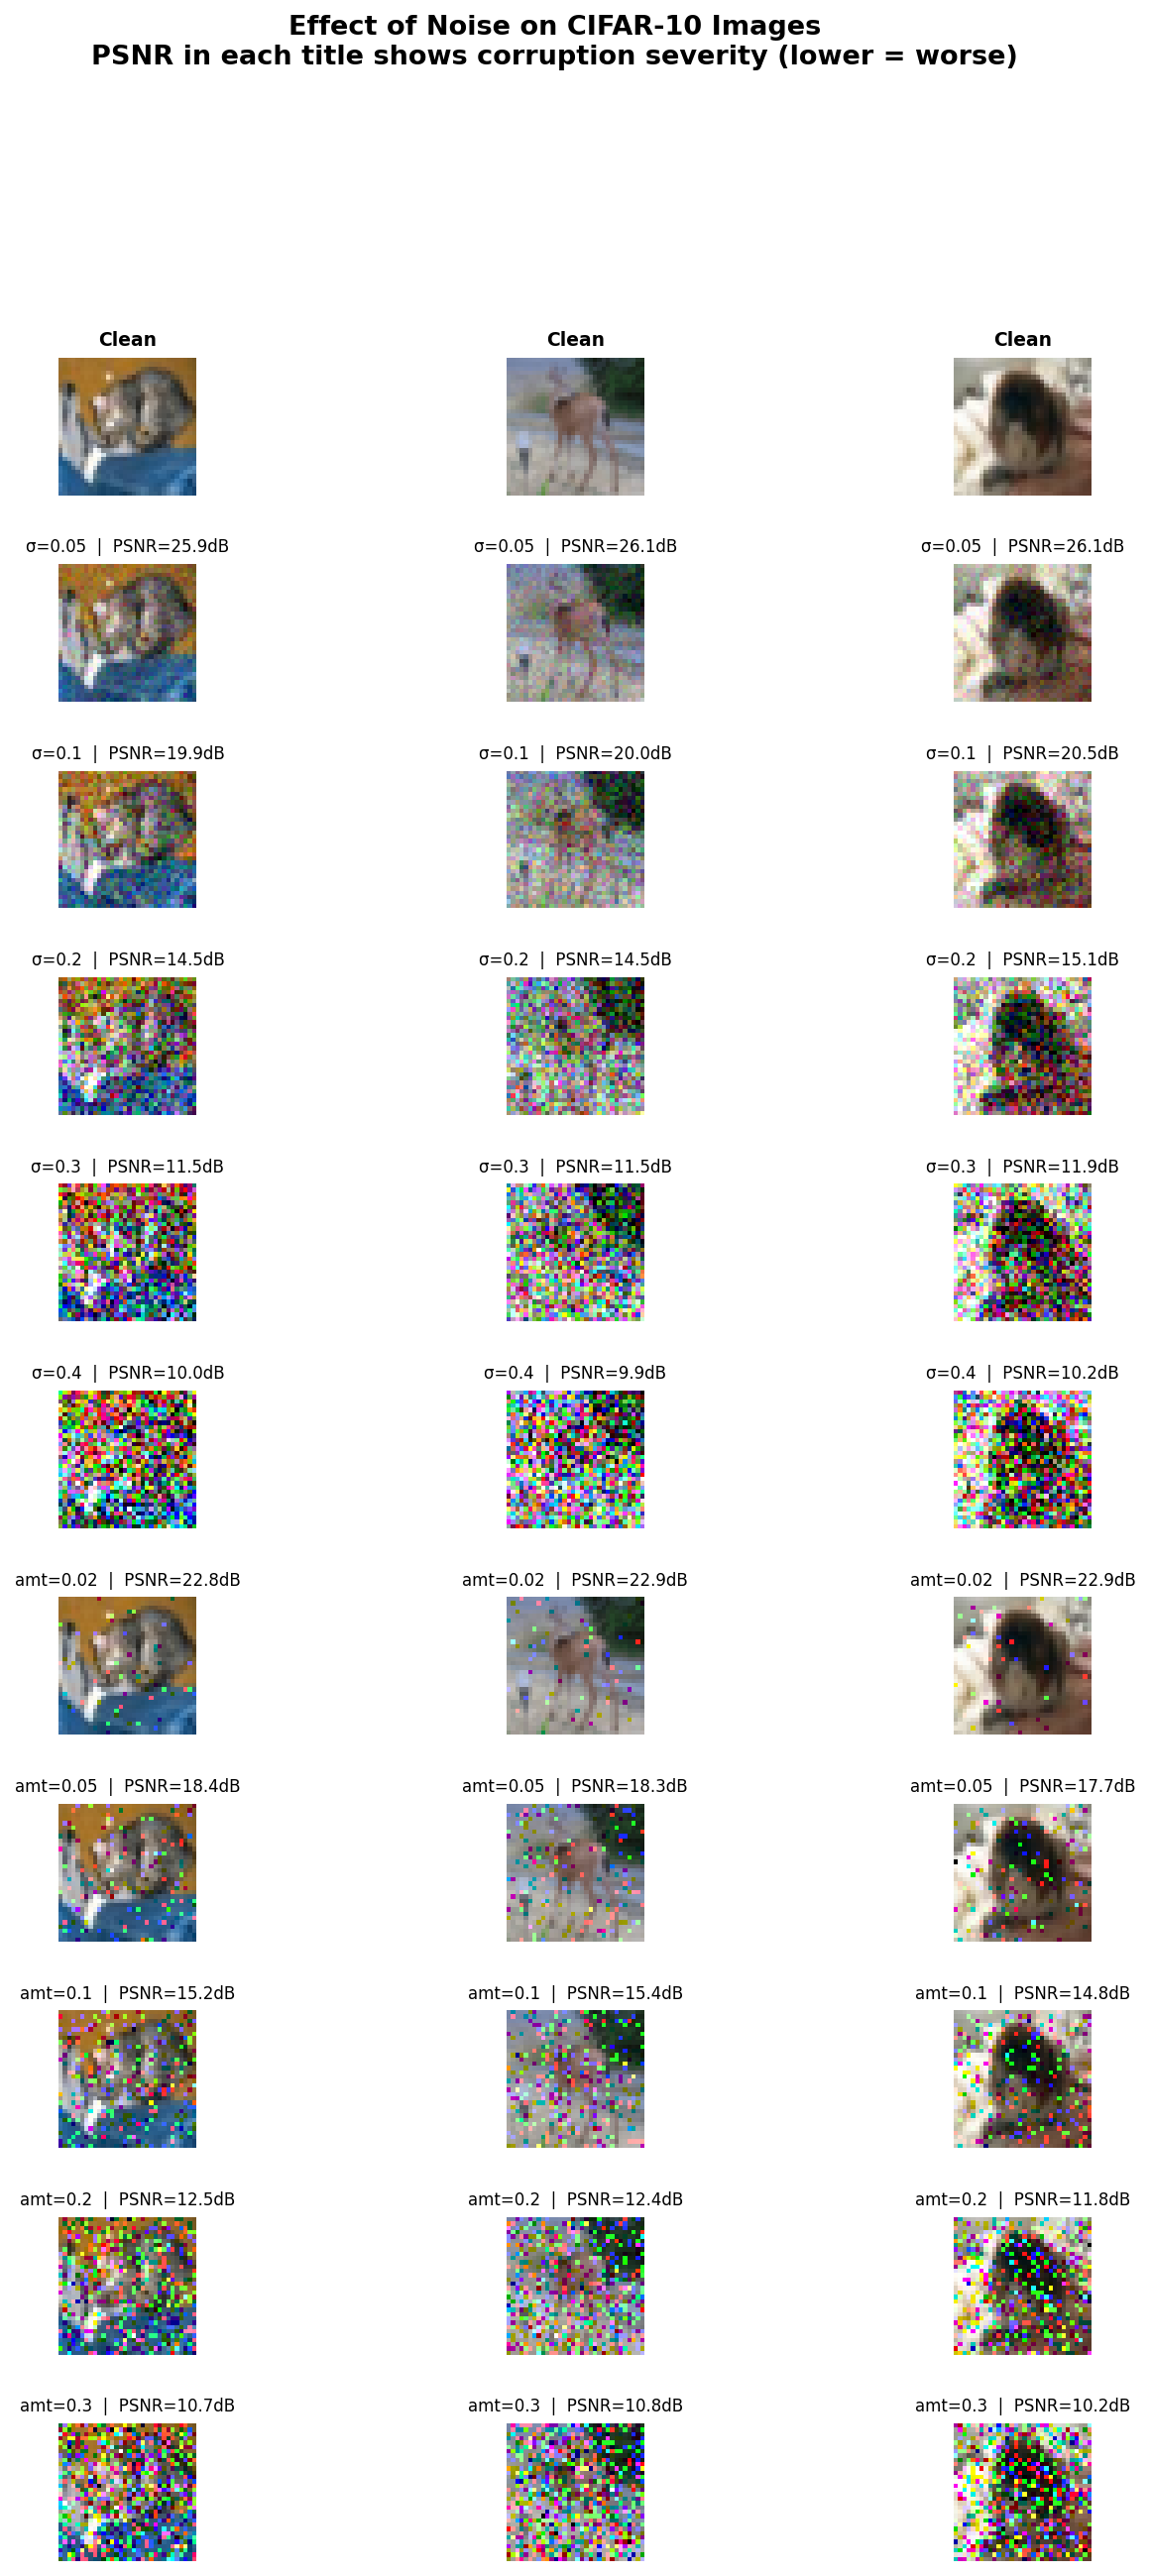
\includegraphics[width=0.90\textwidth]{figures/fig06_noise_level_progression.png}
\caption{Progressive noise corruption: images degraded with increasing noise levels, demonstrating how image content is gradually obscured. At high noise levels ($\sigma > 0.3$, amount $> 0.25$), the original structure becomes barely recognizable.}
\label{fig:noise_progression}
\end{figure}

\begin{figure}[H]
\centering
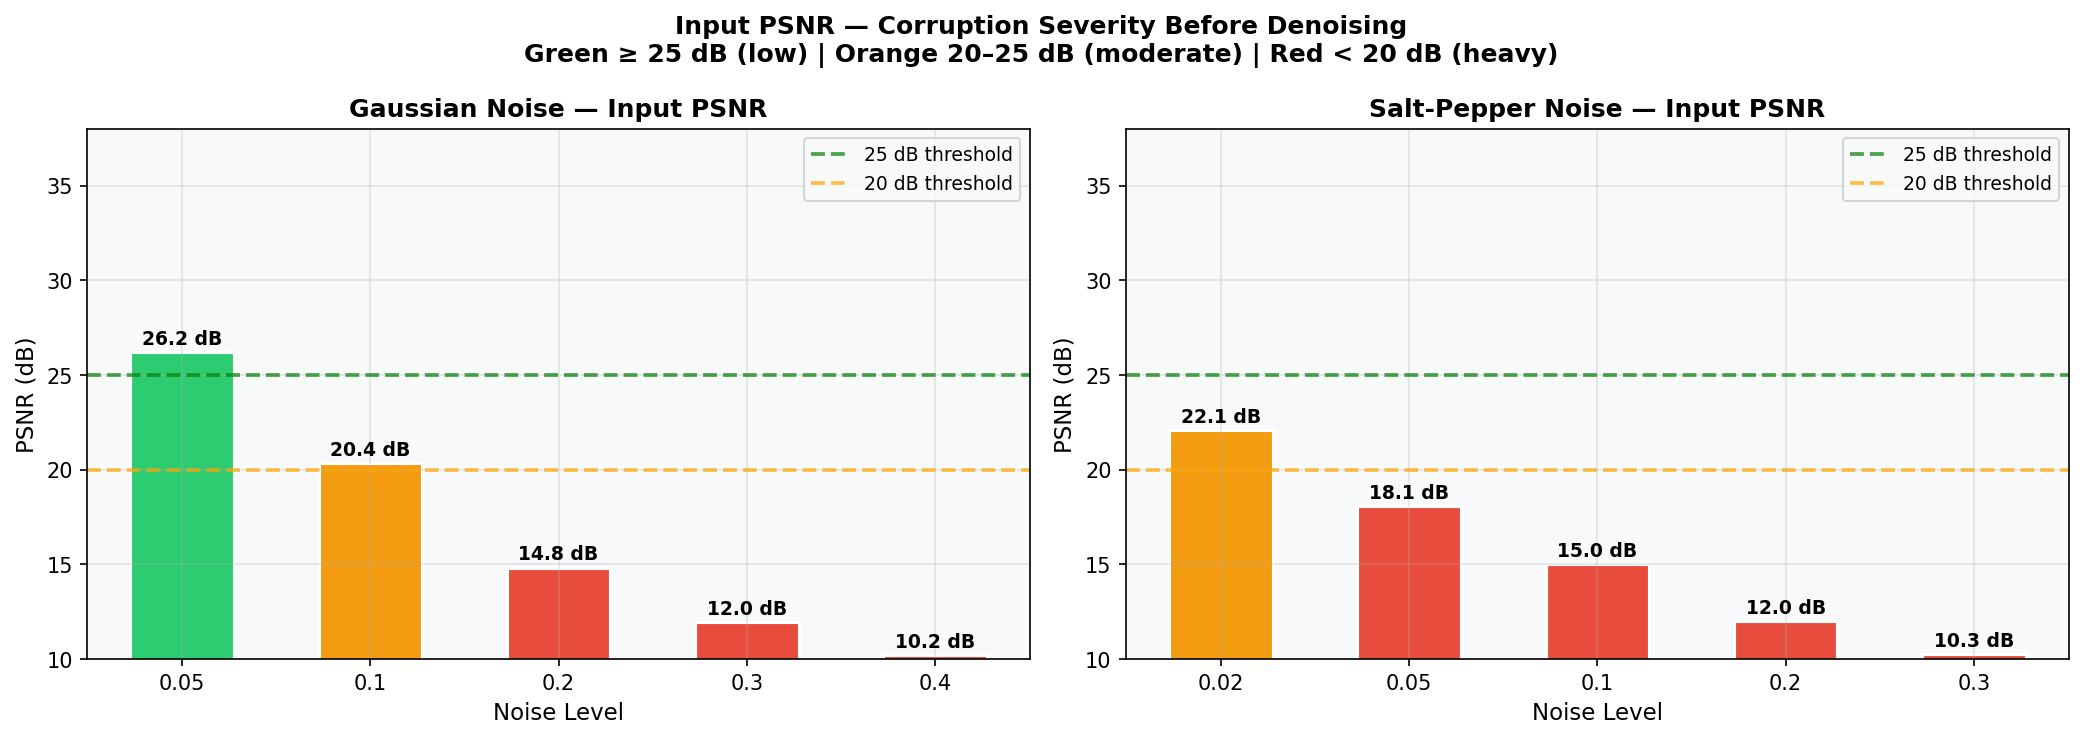
\includegraphics[width=0.80\textwidth]{figures/fig07_input_psnr_bars.png}
\caption{Input PSNR (dB) of noisy images before denoising, measured against clean originals. This serves as the baseline against which reconstruction quality is compared.}
\label{fig:input_psnr}
\end{figure}

\subsection{Training Noise Strategy}
During training, noise is injected \textit{on-the-fly} using a \texttt{NoisyDataset} wrapper class. The default configuration uses Gaussian noise with $\sigma=0.1$. Each time an image is sampled, fresh noise is generated, effectively augmenting the training data and preventing overfitting to specific noise patterns.


% ─────────────────────────────────────────────────────────────────────────
% 5. MODEL ARCHITECTURE
% ─────────────────────────────────────────────────────────────────────────
\section{Model Architecture}
\label{sec:architecture}

The denoising autoencoder is a fully convolutional encoder--decoder network. The architecture consists of 3~encoder blocks and 3~decoder blocks with a configurable bottleneck, as illustrated in Figure~\ref{fig:arch_diagram} and detailed in Table~\ref{tab:arch_summary}.

\subsection{Encoder}
Each encoder block contains:
\begin{enumerate}[nosep]
    \item \texttt{Conv2d} ($3 \times 3$ kernel, padding=1) to learn spatial features.
    \item \texttt{BatchNorm2d} to stabilize gradients and accelerate convergence.
    \item \texttt{ReLU} (inplace) activation for nonlinearity.
    \item \texttt{MaxPool2d} ($2 \times 2$, stride 2) for spatial downsampling.
\end{enumerate}
The channel progression is $3 \to 32 \to 64 \to C_b$ (bottleneck channels), while the spatial dimensions halve at each pooling layer: $32\!\times\!32 \to 16\!\times\!16 \to 8\!\times\!8 \to 4\!\times\!4$.

\subsection{Bottleneck}
The bottleneck tensor has shape $(C_b, 4, 4)$, giving $C_b \times 16$ latent units. With the default $C_b = 128$, this yields \textbf{2{,}048 latent units}—a compression ratio of approximately $\frac{3 \times 32 \times 32}{2048} = 1.5\times$, forcing the encoder to discard noise and retain only the essential image structure.

\subsection{Decoder}
Each decoder block performs:
\begin{enumerate}[nosep]
    \item \texttt{ConvTranspose2d} ($2 \times 2$ kernel, stride 2) for learnable upsampling.
    \item \textbf{Refinement} \texttt{Conv2d} ($3 \times 3$, padding 1) to suppress checkerboard artifacts.
    \item \texttt{BatchNorm2d} + \texttt{ReLU} (blocks 1 and 2 only).
    \item \texttt{Sigmoid} activation in the final block to constrain output to $[0,1]$.
\end{enumerate}

\subsection{Design Decisions}
\begin{itemize}[nosep]
    \item \textbf{No skip connections}: Unlike U-Net, skipping forces the bottleneck to learn a truly compressed, noise-free representation.
    \item \textbf{Refinement convolutions}: A standard Conv after each transposed Conv reduces the checkerboard artifacts common in naïve upsampling.
    \item \textbf{Sigmoid output}: Constrains pixel values to $[0,1]$, matching the normalized input range without post-processing.
    \item \textbf{Fully convolutional}: No fully-connected layers, resulting in fast inference and fewer parameters.
\end{itemize}

\subsection{Architecture Summary}

\begin{table}[H]
\centering
\caption{Layer-by-layer architecture summary (default bottleneck $C_b = 128$).}
\label{tab:arch_summary}
\begin{tabular}{llr}
\toprule
\textbf{Layer Type} & \textbf{Output Shape} & \textbf{Parameters} \\
\midrule
\multicolumn{3}{c}{\textit{Encoder}} \\
\midrule
Conv2d ($3 \to 32$)       & $(32, 32, 32)$  & 896 \\
BatchNorm2d               & $(32, 32, 32)$  & 64 \\
ReLU                      & $(32, 32, 32)$  & 0 \\
MaxPool2d                 & $(32, 16, 16)$  & 0 \\
Conv2d ($32 \to 64$)      & $(64, 16, 16)$  & 18{,}496 \\
BatchNorm2d               & $(64, 16, 16)$  & 128 \\
ReLU                      & $(64, 16, 16)$  & 0 \\
MaxPool2d                 & $(64, 8, 8)$    & 0 \\
Conv2d ($64 \to 128$)     & $(128, 8, 8)$   & 73{,}856 \\
BatchNorm2d               & $(128, 8, 8)$   & 256 \\
ReLU                      & $(128, 8, 8)$   & 0 \\
MaxPool2d                 & $(128, 4, 4)$   & 0 \\
\midrule
\multicolumn{3}{c}{\textit{Bottleneck: $(128, 4, 4) = 2{,}048$ latent units}} \\
\midrule
\multicolumn{3}{c}{\textit{Decoder}} \\
\midrule
ConvTranspose2d ($128 \to 64$) & $(64, 8, 8)$    & 32{,}832 \\
Conv2d ($64 \to 64$)           & $(64, 8, 8)$    & 36{,}928 \\
BatchNorm2d                    & $(64, 8, 8)$    & 128 \\
ReLU                           & $(64, 8, 8)$    & 0 \\
ConvTranspose2d ($64 \to 32$)  & $(32, 16, 16)$  & 8{,}224 \\
Conv2d ($32 \to 32$)           & $(32, 16, 16)$  & 9{,}248 \\
BatchNorm2d                    & $(32, 16, 16)$  & 64 \\
ReLU                           & $(32, 16, 16)$  & 0 \\
ConvTranspose2d ($32 \to 3$)   & $(3, 32, 32)$   & 387 \\
Conv2d ($3 \to 3$)             & $(3, 32, 32)$   & 84 \\
Sigmoid                        & $(3, 32, 32)$   & 0 \\
\midrule
\multicolumn{2}{l}{\textbf{Total Parameters}} & \textbf{181{,}591} \\
\multicolumn{2}{l}{Trainable Parameters}      & 181{,}591 \\
\bottomrule
\end{tabular}
\end{table}

\begin{figure}[H]
\centering
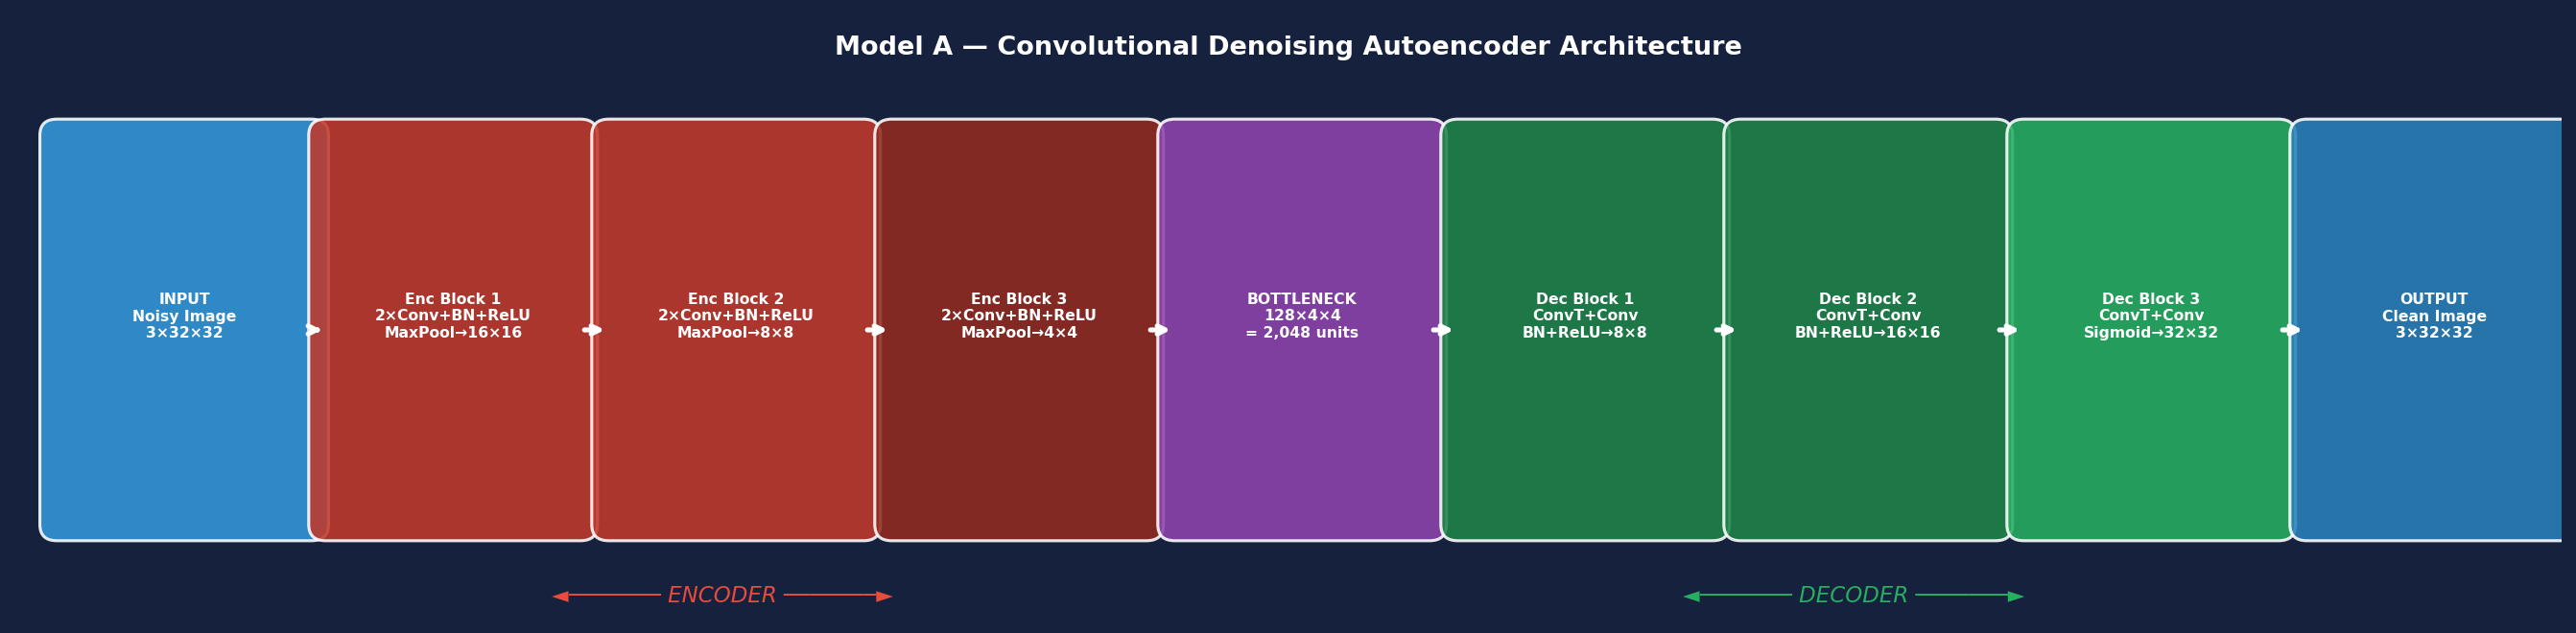
\includegraphics[width=0.85\textwidth]{figures/fig08_architecture_diagram.png}
\caption{Architecture block diagram of the Denoising Autoencoder showing the encoder pathway (left), bottleneck (center), and decoder pathway (right) with channel and spatial dimensions labeled at each stage.}
\label{fig:arch_diagram}
\end{figure}

\begin{figure}[H]
\centering
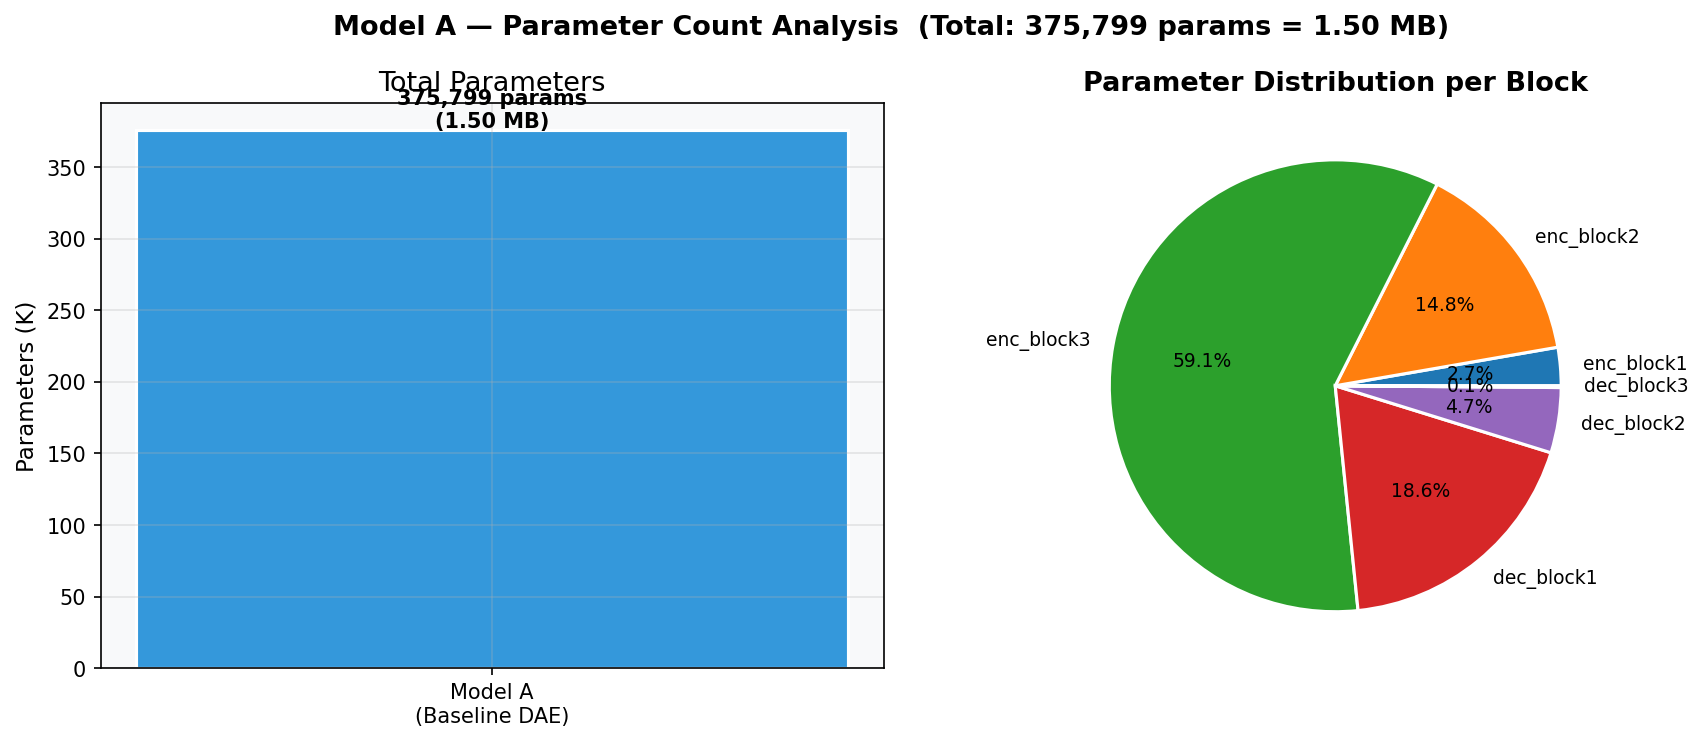
\includegraphics[width=0.80\textwidth]{figures/fig09_parameter_analysis.png}
\caption{Parameter distribution analysis. The encoder's third convolutional layer (64$\to$128) contributes the most parameters due to the large number of filters. The decoder's refinement convolutions add only modest overhead.}
\label{fig:param_analysis}
\end{figure}


% ─────────────────────────────────────────────────────────────────────────
% 6. MODEL TRAINING
% ─────────────────────────────────────────────────────────────────────────
\section{Model Training}
\label{sec:training}

\subsection{Loss Function}
The model is trained to minimize the \textbf{Mean Squared Error (MSE)} between the reconstructed output and the clean target image:
\begin{equation}
    \mathcal{L}_{\text{MSE}} = \frac{1}{N} \sum_{i=1}^{N} \| \hat{x}_i - x_i \|^2
\end{equation}
where $x_i$ is the clean image, $\hat{x}_i = f_\theta(x_i + \text{noise})$ is the model's reconstruction, and $N$ is the number of pixels.

MSE is chosen because it directly penalizes pixel-level deviations and is smooth, convex, and differentiable everywhere—ideal for gradient-based optimization.

\subsection{Training Procedure}
Table~\ref{tab:training_config} summarizes the training configuration.

\begin{table}[H]
\centering
\caption{Training hyperparameters.}
\label{tab:training_config}
\begin{tabular}{ll}
\toprule
\textbf{Hyperparameter}   & \textbf{Value} \\
\midrule
Optimizer                  & Adam~\cite{kingma2014adam} (weight\_decay=$10^{-5}$) \\
Learning rate              & $1 \times 10^{-3}$ \\
LR Scheduler               & ReduceLROnPlateau (factor=0.5, patience=5) \\
Batch size                 & 128 \\
Number of epochs           & 30 \\
Loss function              & MSELoss \\
Noise (training)           & Gaussian $\sigma=0.1$ (on-the-fly via NoisyDataset) \\
Best-model selection       & Lowest validation loss \\
\bottomrule
\end{tabular}
\end{table}

\subsection{Training and Validation Loss Curves}
Figure~\ref{fig:training_dashboard} shows the comprehensive training dashboard including loss curves, learning rate schedule, and best epoch selection. Both training and validation losses decrease steadily, with the validation loss closely tracking the training loss, indicating minimal overfitting.

\begin{figure}[H]
\centering
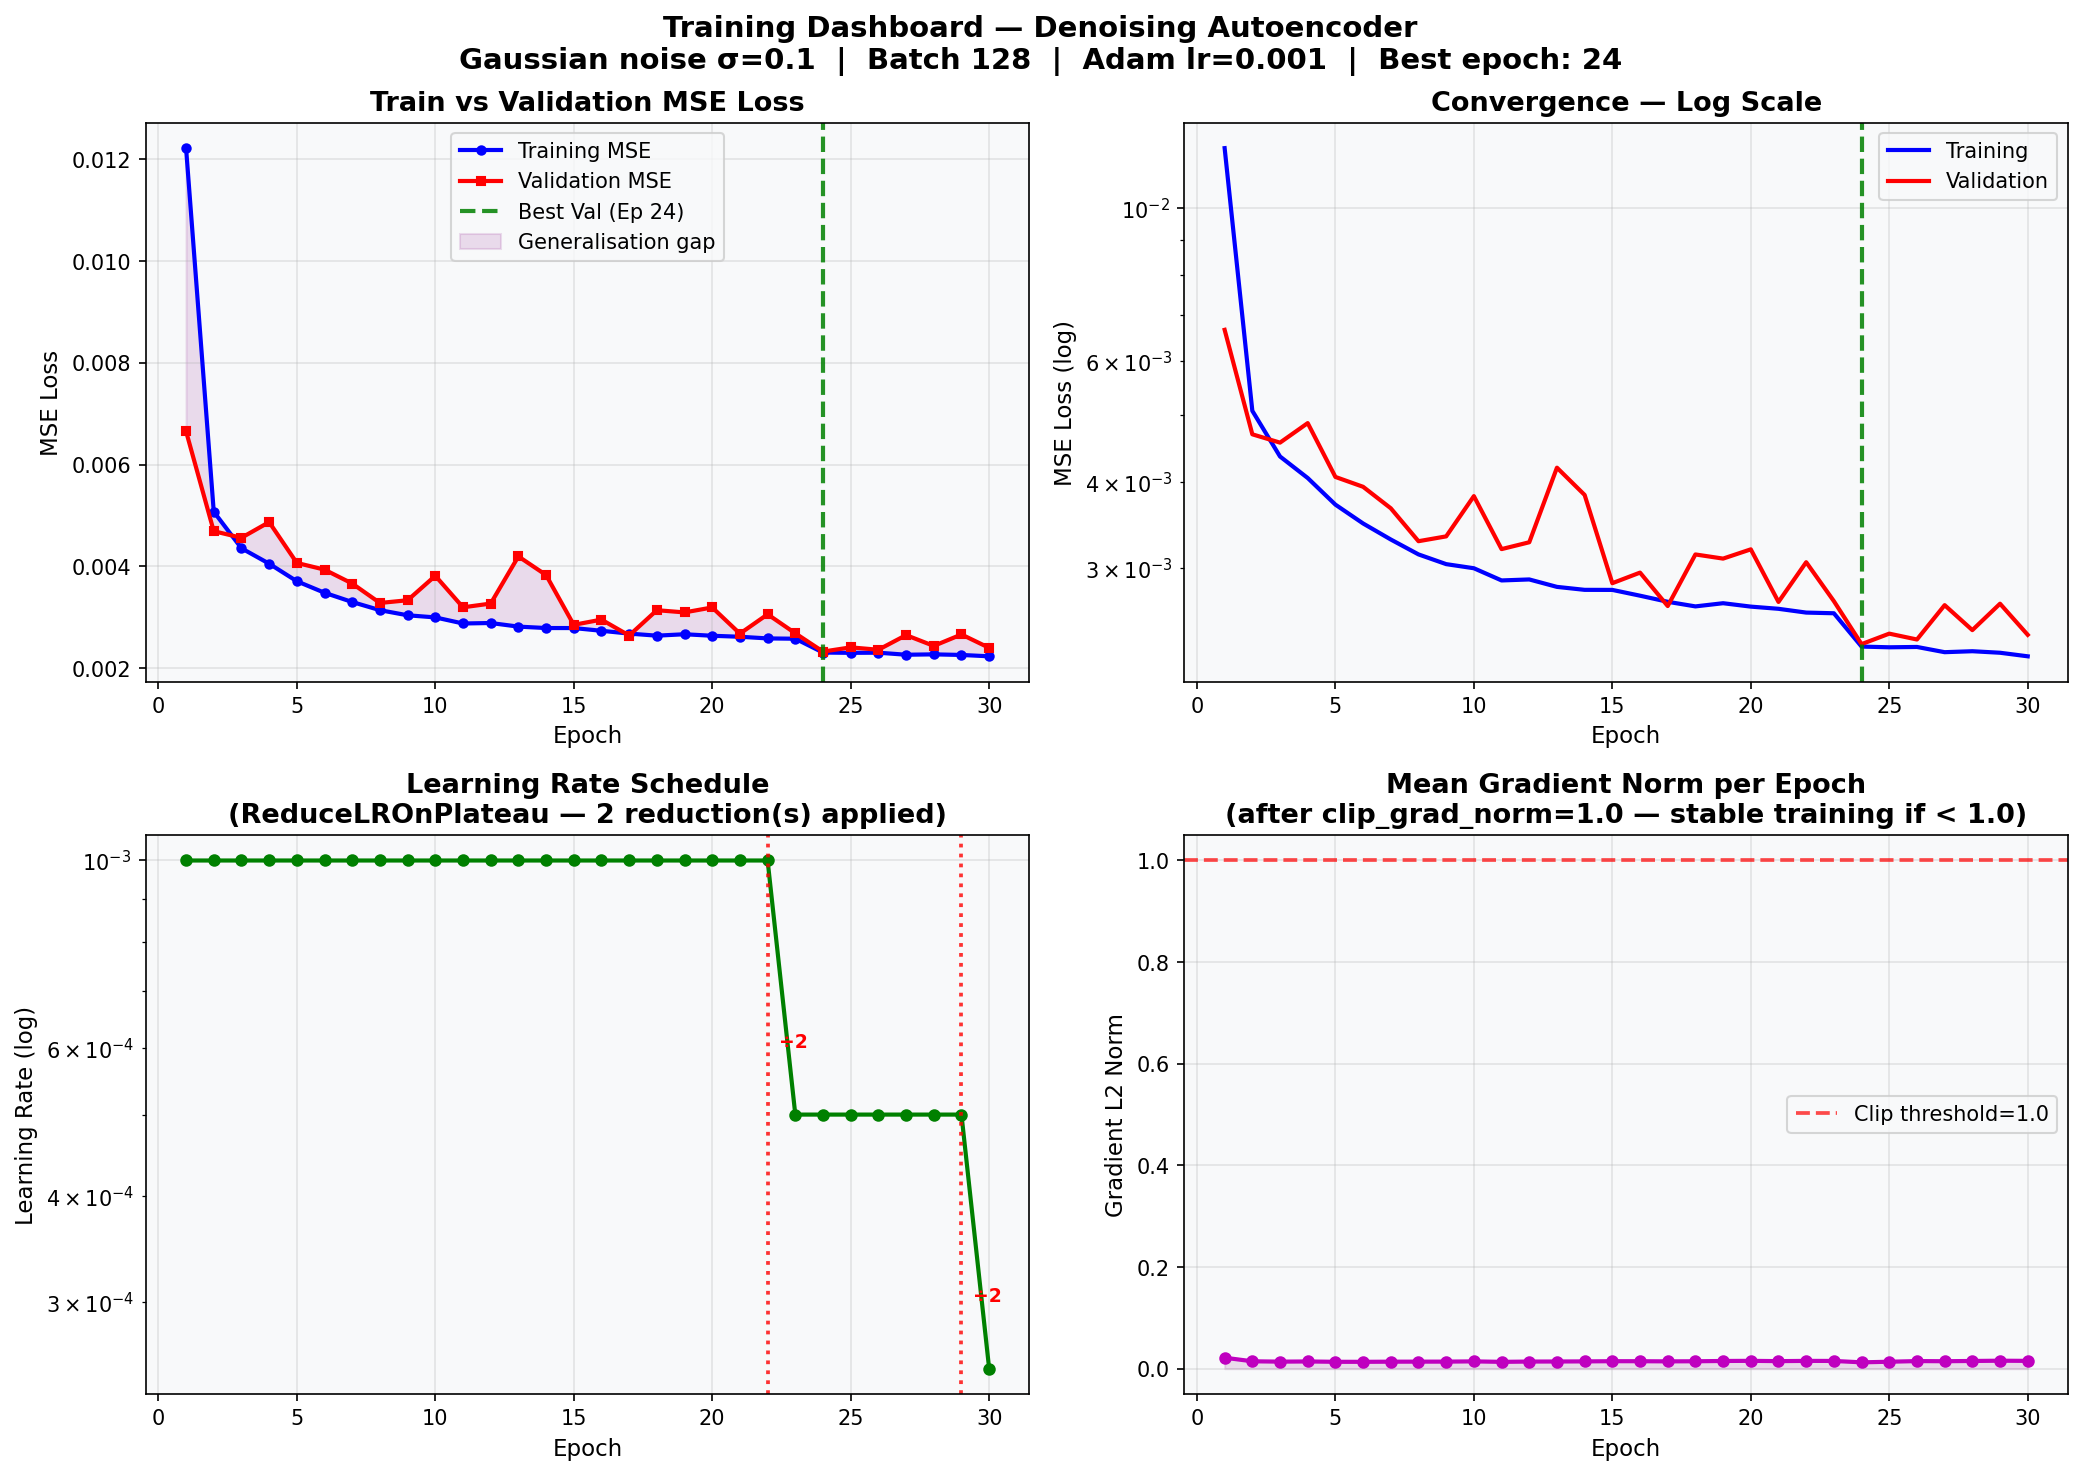
\includegraphics[width=0.90\textwidth]{figures/fig10_training_dashboard.png}
\caption{Training dashboard showing: (1) training and validation MSE loss curves over 30 epochs, (2) learning rate schedule with ReduceLROnPlateau adjustments, and (3) best model checkpoint selection (marked with a star).}
\label{fig:training_dashboard}
\end{figure}


% ─────────────────────────────────────────────────────────────────────────
% 7. EVALUATION AND VISUALIZATION
% ─────────────────────────────────────────────────────────────────────────
\section{Evaluation and Visualization}
\label{sec:evaluation}

\subsection{Reconstruction Metrics}
The trained model is evaluated on the held-out test set (10{,}000 images) using three metrics:

\begin{itemize}[nosep]
    \item \textbf{MSE (Mean Squared Error)}: Average squared pixel difference. Lower is better.
    \item \textbf{PSNR (Peak Signal-to-Noise Ratio)}: Measures reconstruction fidelity in decibels. Higher is better. Computed as:
    \begin{equation}
        \text{PSNR} = 10 \cdot \log_{10}\!\left(\frac{\text{MAX}^2}{\text{MSE}}\right) \quad \text{where MAX} = 1.0
    \end{equation}
    \item \textbf{SSIM (Structural Similarity Index)}: Measures perceptual similarity considering luminance, contrast, and structure. Range $[-1, 1]$; higher is better.
\end{itemize}

Table~\ref{tab:test_metrics} presents the test-set results for the default configuration (bottleneck$=128$, Gaussian $\sigma=0.1$).

\begin{table}[H]
\centering
\caption{Test set reconstruction metrics (default model, Gaussian $\sigma=0.1$).}
\label{tab:test_metrics}
\begin{tabular}{lc}
\toprule
\textbf{Metric} & \textbf{Value} \\
\midrule
MSE          & 0.003784 \\
PSNR         & 24.62 dB \\
SSIM         & 0.8225 \\
\bottomrule
\end{tabular}
\end{table}

\subsection{Denoising Visualization}
Figure~\ref{fig:denoising_results} displays a comprehensive grid of denoising results showing original, noisy, and reconstructed images side by side.

\begin{figure}[H]
\centering
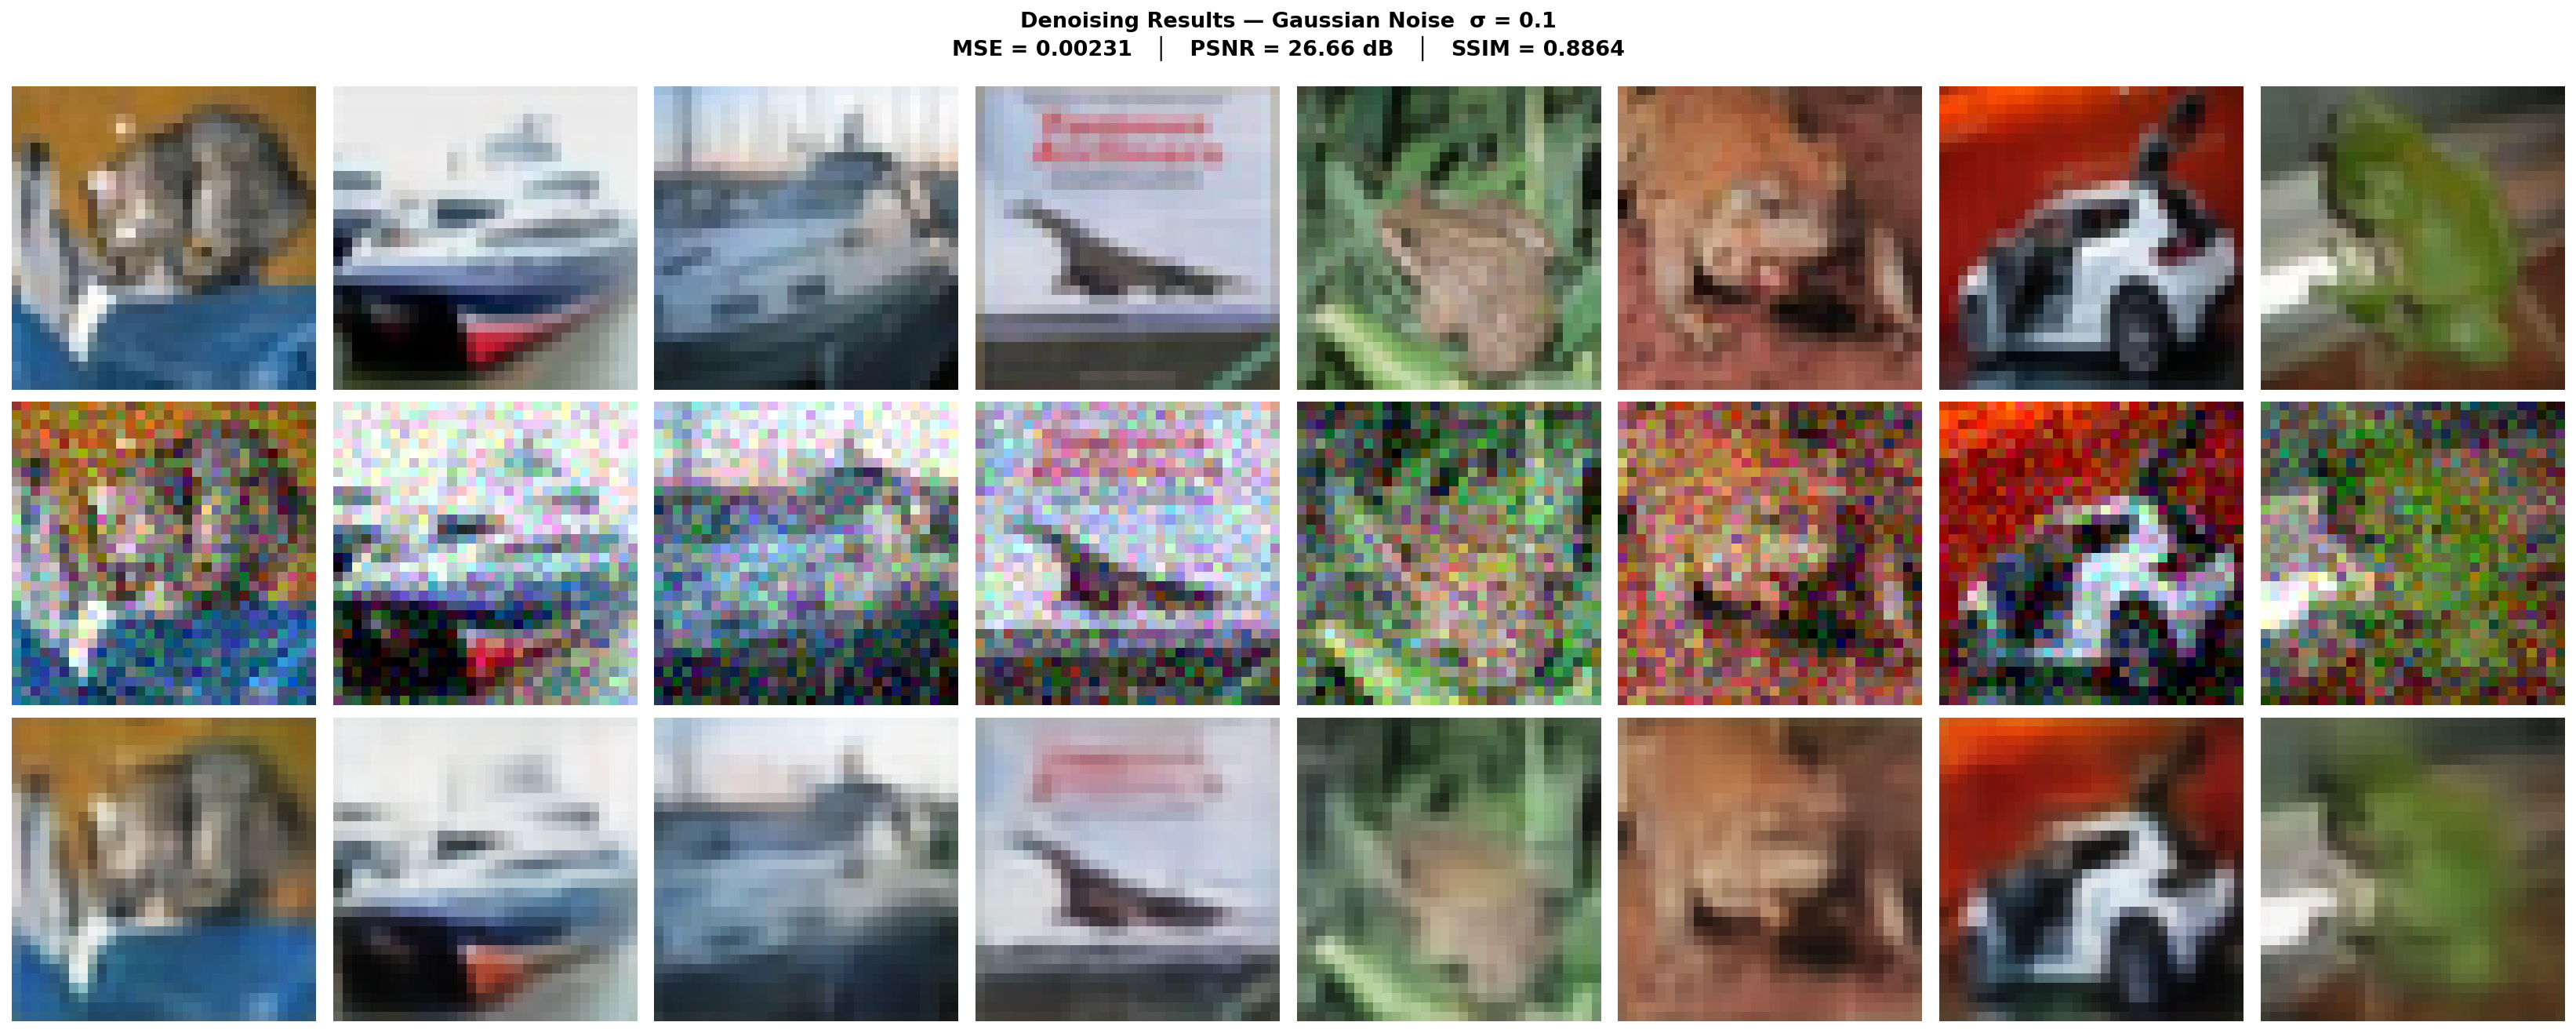
\includegraphics[width=0.95\textwidth]{figures/fig11_denoising_results_grid.png}
\caption{Denoising results grid. Row~1: Original clean images. Row~2: Noisy inputs (Gaussian $\sigma=0.1$). Row~3: Reconstructed (denoised) images. The model successfully removes noise while preserving the overall structure and colors.}
\label{fig:denoising_results}
\end{figure}

\subsection{Error Analysis}
Figure~\ref{fig:error_maps} shows pixel-wise absolute error heatmaps between reconstructed and clean images, revealing where the model struggles most (typically edges and fine textures).

\begin{figure}[H]
\centering
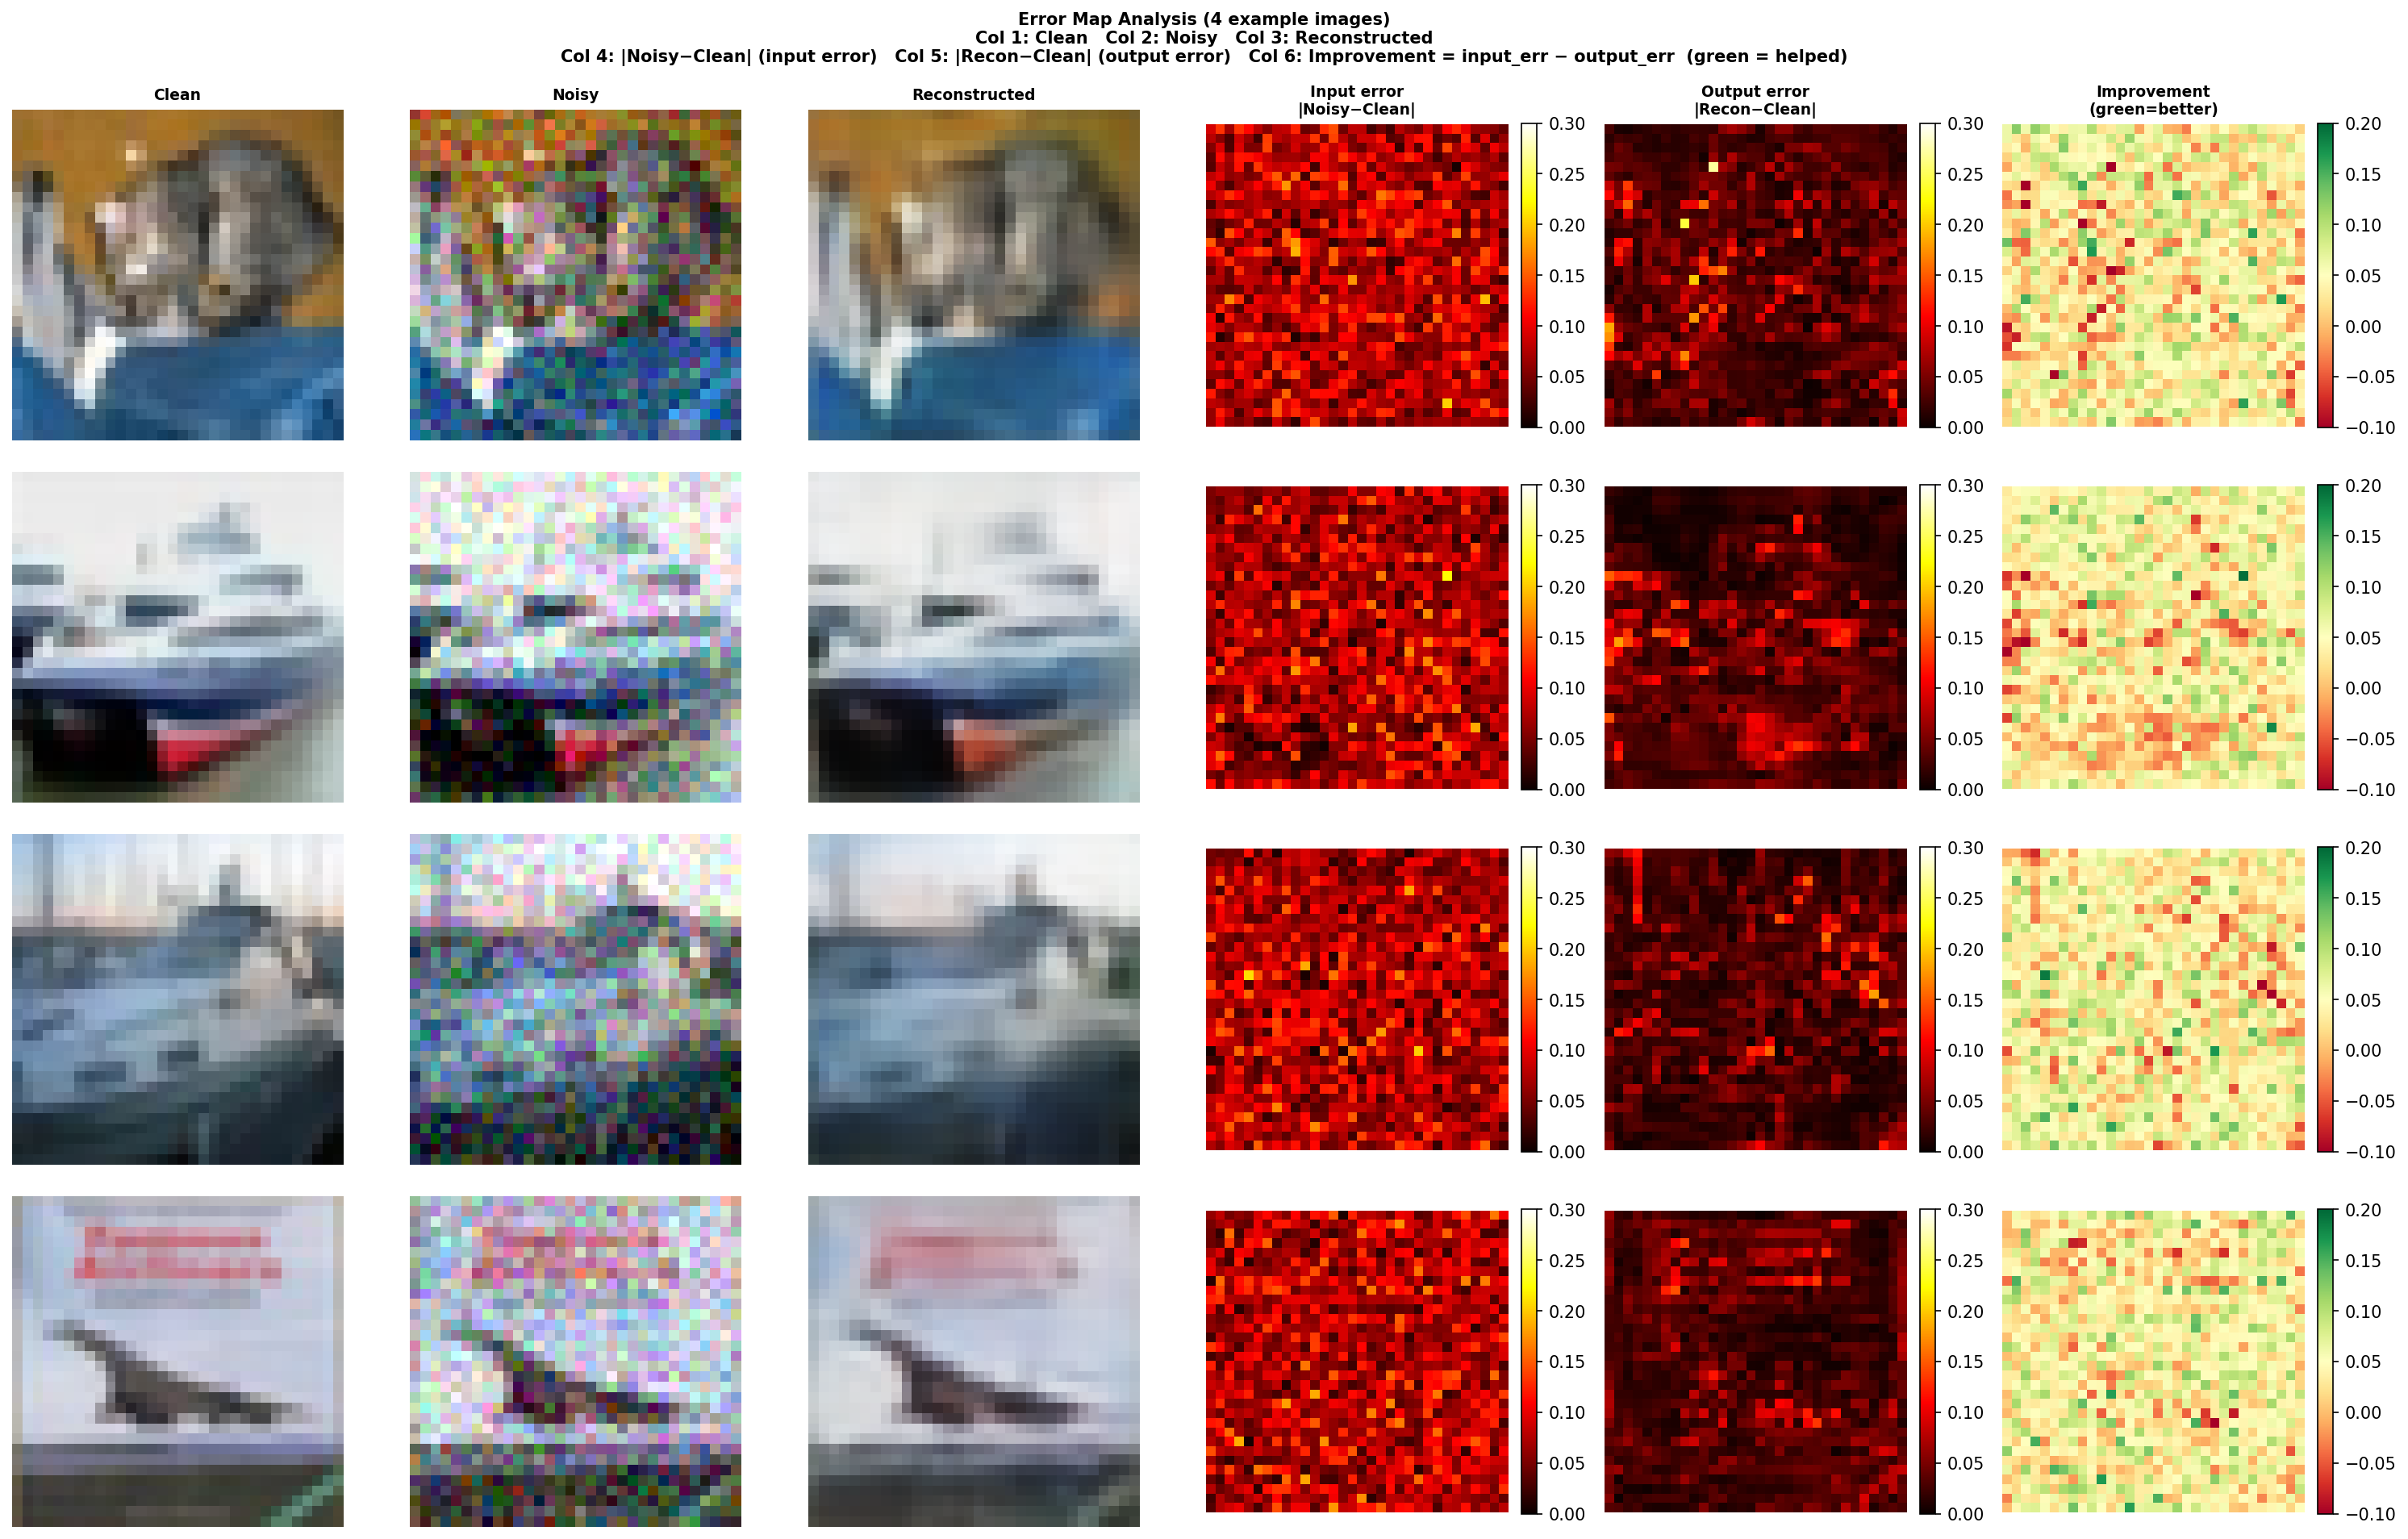
\includegraphics[width=0.90\textwidth]{figures/fig12_error_maps.png}
\caption{Pixel-wise absolute error maps. Brighter regions indicate higher reconstruction error. Errors concentrate along object edges and high-frequency texture regions, consistent with the MSE loss's tendency to produce locally averaged (blurry) predictions.}
\label{fig:error_maps}
\end{figure}

\subsection{Metric Distributions}
Figure~\ref{fig:metric_distributions} shows the distributions of per-image PSNR and SSIM values across the full test set, demonstrating consistent reconstruction quality.

\begin{figure}[H]
\centering
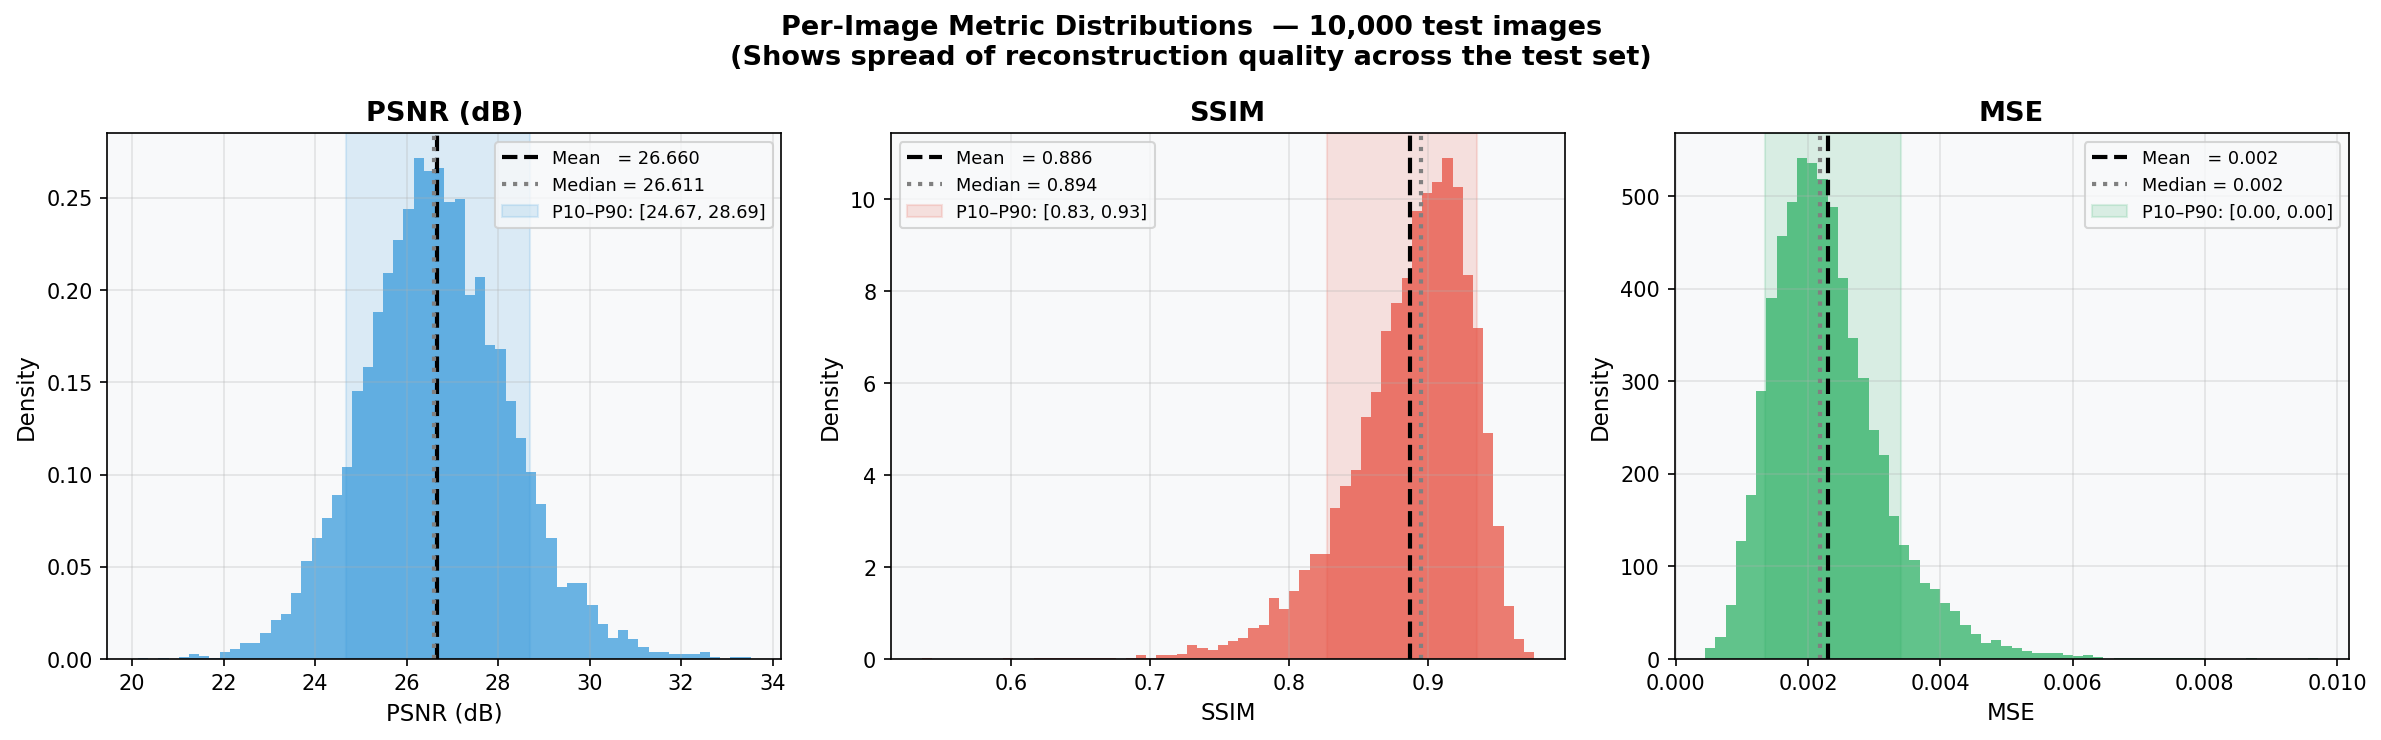
\includegraphics[width=0.85\textwidth]{figures/fig13_metric_distributions.png}
\caption{Per-image PSNR and SSIM distributions over the 10{,}000 test images. The tight distributions (low variance) indicate that the model performs consistently across diverse image content.}
\label{fig:metric_distributions}
\end{figure}

\subsection{Per-Class Performance}
Figure~\ref{fig:per_class_metrics} breaks down reconstruction quality by CIFAR-10 class, revealing that classes with more uniform backgrounds (``frog,'' ``ship'') tend to achieve higher PSNR, while classes with complex textures (``cat,'' ``deer'') score lower.

\begin{figure}[H]
\centering
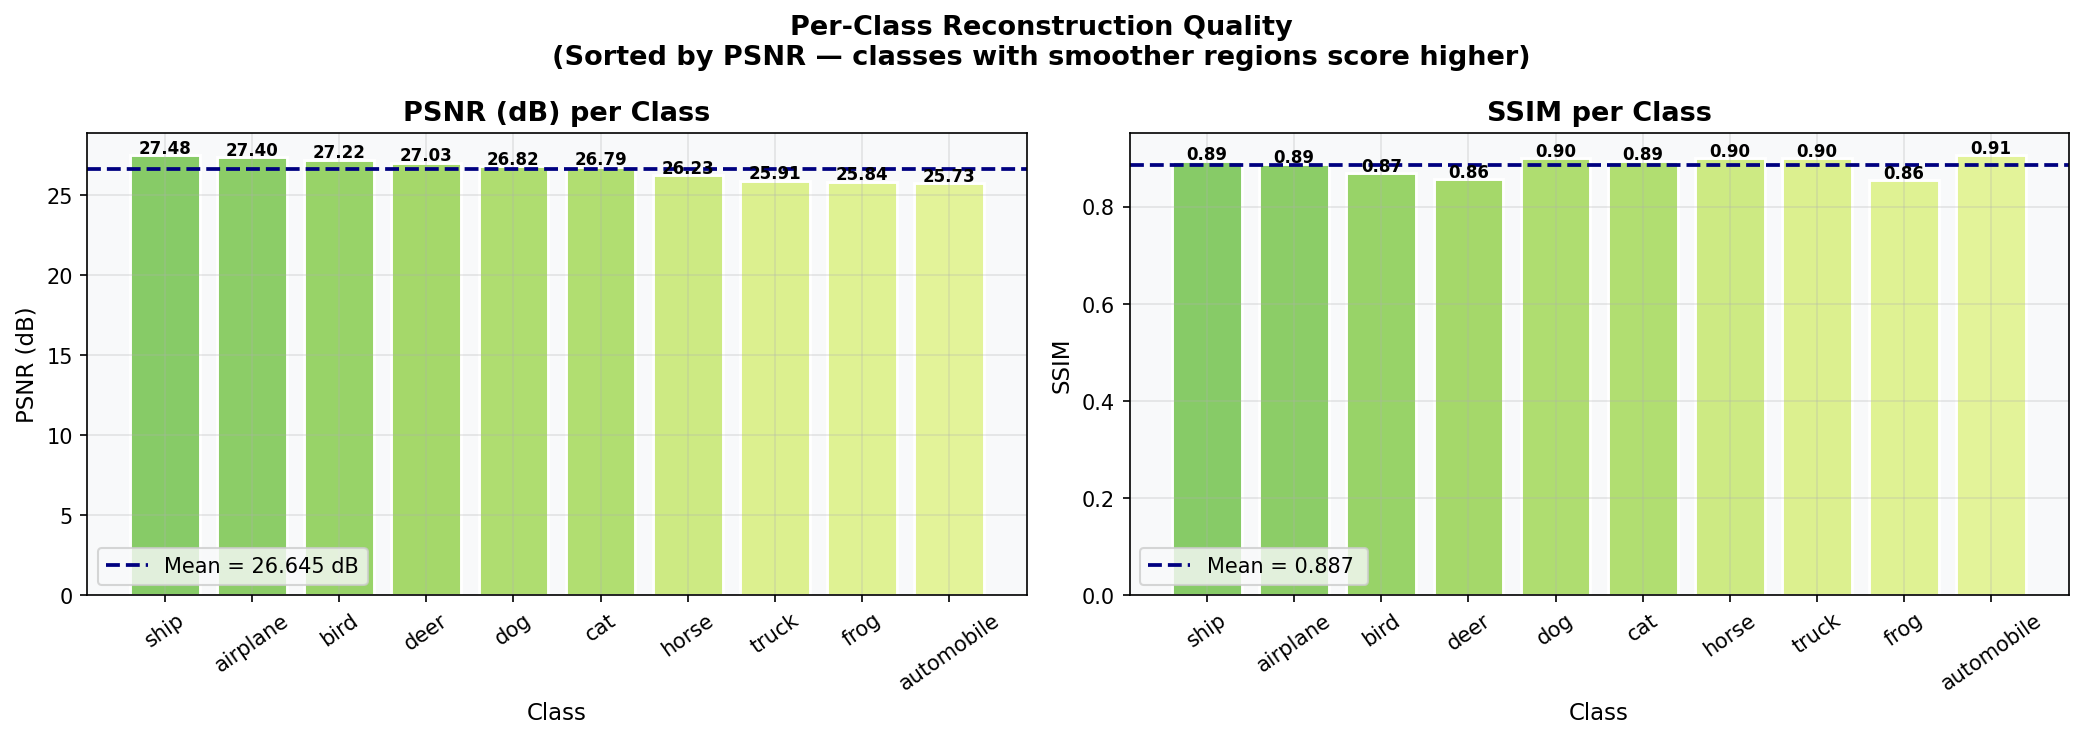
\includegraphics[width=0.85\textwidth]{figures/fig14_per_class_metrics.png}
\caption{Per-class reconstruction metrics. Classes with simpler visual patterns (e.g., ``frog'' with green backgrounds) achieve higher PSNR/SSIM than classes with complex textures and fine-grained features (e.g., ``cat'' with fur patterns).}
\label{fig:per_class_metrics}
\end{figure}

\subsection{Frequency Domain Analysis}
Figure~\ref{fig:fft_analysis} shows the FFT (Fast Fourier Transform) analysis of clean, noisy, and denoised images, illustrating how the autoencoder acts as a low-pass filter.

\begin{figure}[H]
\centering
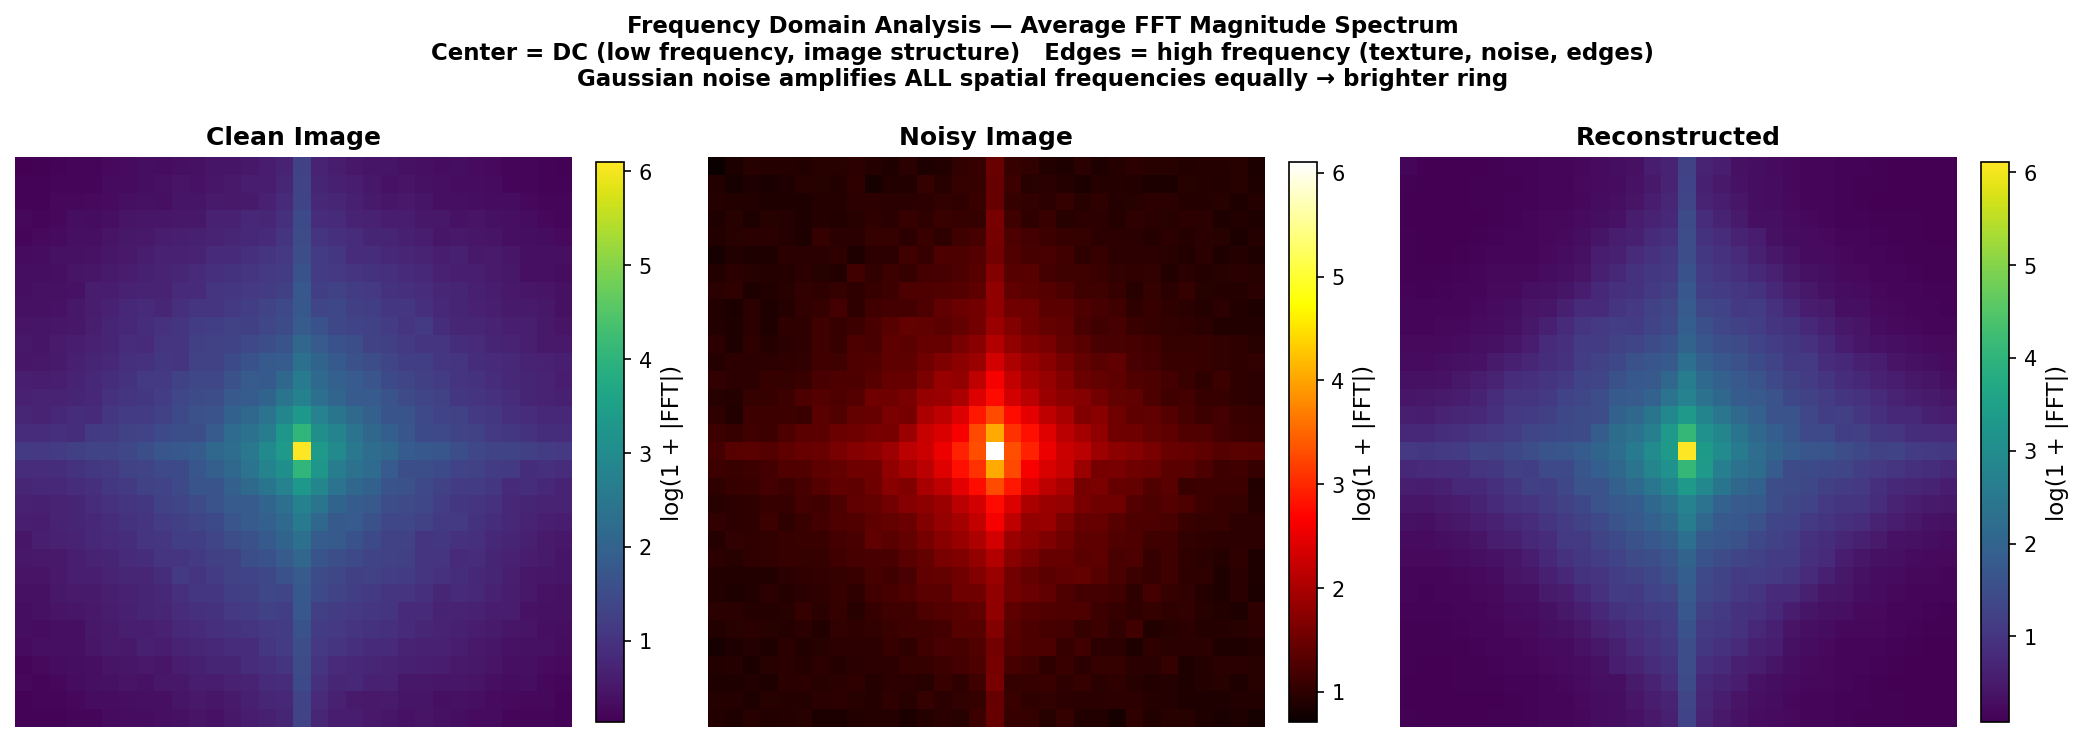
\includegraphics[width=0.85\textwidth]{figures/fig15_fft_analysis.png}
\caption{Frequency domain (FFT) analysis. The power spectrum of noisy images shows elevated high-frequency energy (flat noise floor). The denoised images exhibit reduced high-frequency content compared to even the clean originals, confirming the autoencoder's role as a learned low-pass filter.}
\label{fig:fft_analysis}
\end{figure}


% ─────────────────────────────────────────────────────────────────────────
% 8. EXPERIMENTAL STUDY
% ─────────────────────────────────────────────────────────────────────────
\section{Experimental Study}
\label{sec:experiments}

Two experiments are conducted to analyze how reconstruction performance varies with (A)~noise level and (B)~bottleneck size.

\subsection{Experiment A — Noise Level Sensitivity}
\label{sec:exp_a}

\textbf{Setup}: Fixed bottleneck $= 128$ channels. Each configuration is trained for 15~epochs. Noise levels are varied independently for Gaussian and salt-and-pepper noise.

\subsubsection{Gaussian Noise Results}

\begin{table}[H]
\centering
\caption{Reconstruction quality vs.\ Gaussian noise level ($\sigma$).}
\label{tab:exp_a_gauss}
\begin{tabular}{cccc}
\toprule
$\sigma$ & \textbf{MSE} & \textbf{PSNR (dB)} & \textbf{SSIM} \\
\midrule
0.05 & 0.0039 & 24.49 & 0.8202 \\
0.10 & 0.0044 & 23.93 & 0.7966 \\
0.20 & 0.0056 & 22.82 & 0.7458 \\
0.30 & 0.0072 & 21.70 & 0.6854 \\
0.40 & 0.0088 & 20.80 & 0.6417 \\
\bottomrule
\end{tabular}
\end{table}

\subsubsection{Salt-and-Pepper Noise Results}

\begin{table}[H]
\centering
\caption{Reconstruction quality vs.\ salt-and-pepper noise amount.}
\label{tab:exp_a_sp}
\begin{tabular}{cccc}
\toprule
\textbf{Amount} & \textbf{MSE} & \textbf{PSNR (dB)} & \textbf{SSIM} \\
\midrule
0.02 & 0.0043 & 24.12 & 0.8084 \\
0.05 & 0.0044 & 23.98 & 0.8013 \\
0.10 & 0.0044 & 23.92 & 0.7981 \\
0.20 & 0.0049 & 23.51 & 0.7755 \\
0.30 & 0.0054 & 23.07 & 0.7579 \\
\bottomrule
\end{tabular}
\end{table}

\begin{figure}[H]
\centering
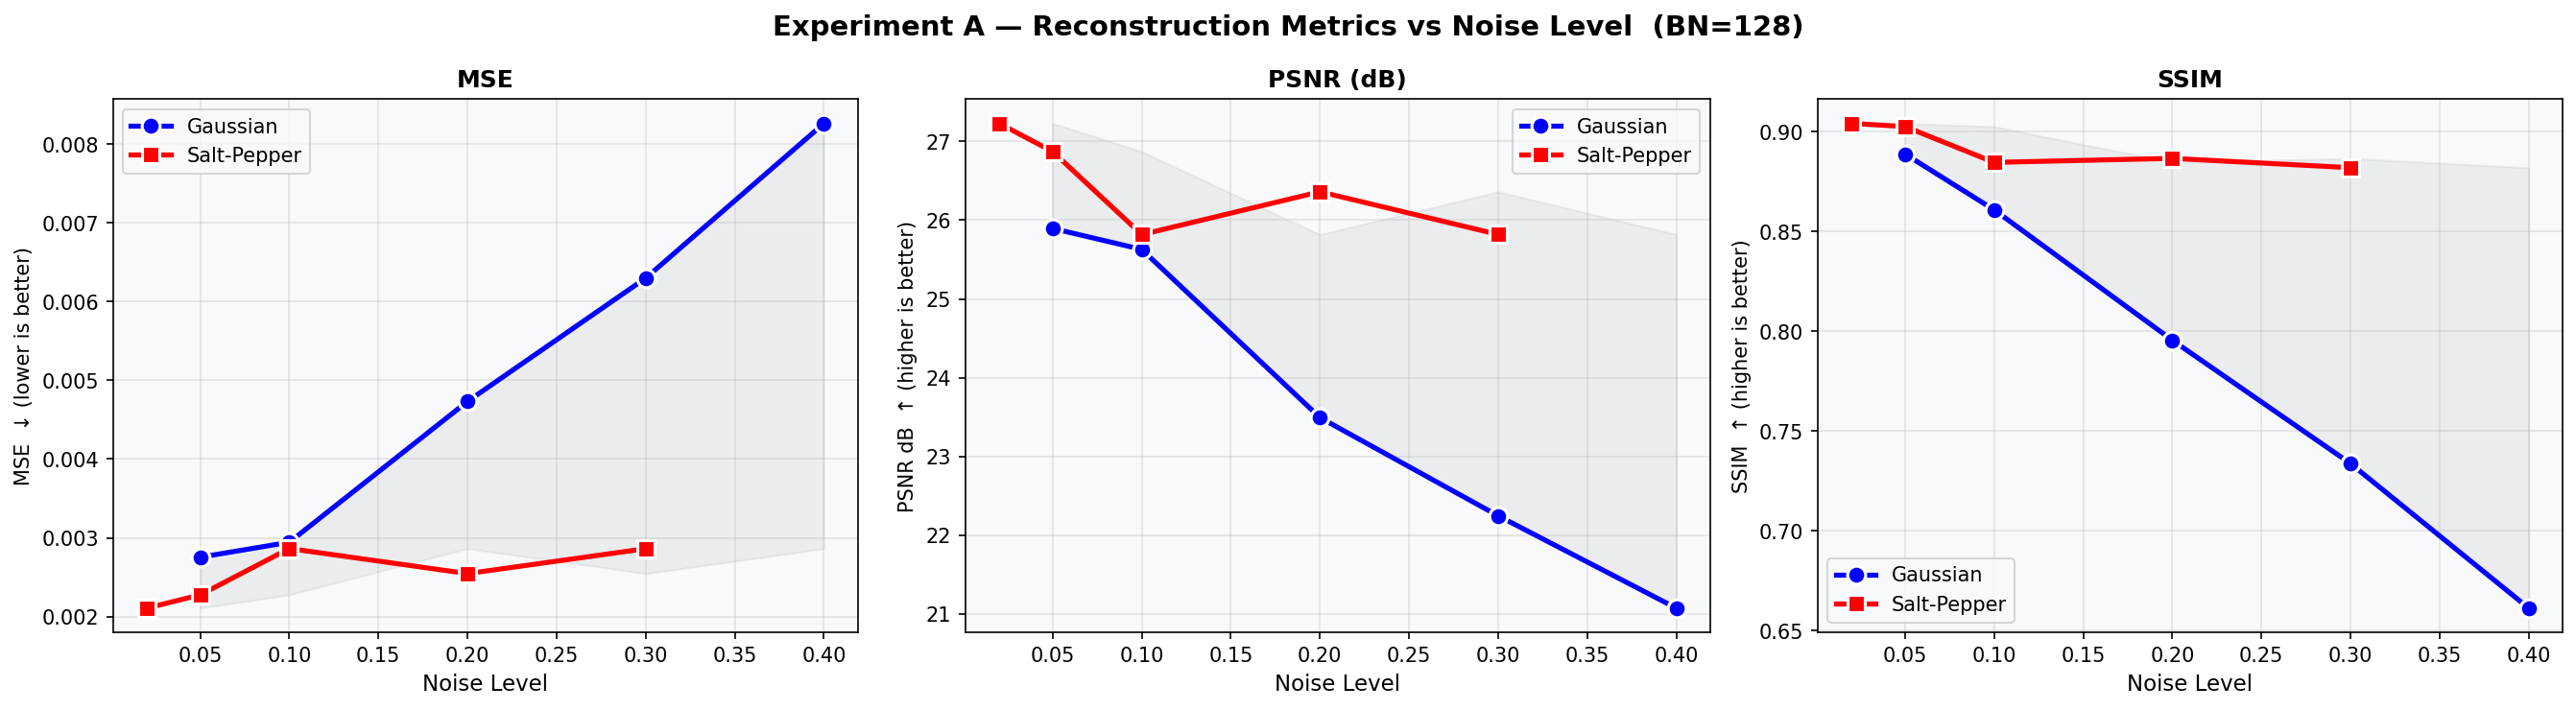
\includegraphics[width=0.95\textwidth]{figures/fig17_exp_A_noise_levels.png}
\caption{Experiment A results: MSE, PSNR, and SSIM vs.\ noise level for both Gaussian and salt-and-pepper noise (bottleneck $= 128$). Gaussian noise degrades quality more steeply than salt-and-pepper at equivalent levels.}
\label{fig:exp_noise}
\end{figure}

\textbf{Key Observations:}
\begin{itemize}[nosep]
    \item As Gaussian $\sigma$ increases, PSNR decreases and MSE increases approximately quadratically.
    \item Salt-and-pepper noise is comparatively easier to denoise because it is spatially sparse—intact neighboring pixels provide strong reconstruction cues.
    \item Even at severe corruption ($\sigma=0.3$ or amt$=0.3$), the autoencoder produces visually plausible images, though fine details are lost.
\end{itemize}

\subsection{Experiment B — Bottleneck Size Impact}
\label{sec:exp_b}

\textbf{Setup}: Fixed Gaussian noise $\sigma = 0.1$. Bottleneck channels varied across $\{16, 32, 64, 128, 256\}$. Each model trained for 15~epochs.

\begin{table}[H]
\centering
\caption{Reconstruction quality vs.\ bottleneck size (Gaussian $\sigma=0.1$).}
\label{tab:exp_b}
\begin{tabular}{cccccc}
\toprule
\textbf{BN} & \textbf{Latent Units} & \textbf{Params} & \textbf{MSE} & \textbf{PSNR (dB)} & \textbf{SSIM} \\
\midrule
16  & 256  & 88{,}071  & 0.0067 & 22.25 & 0.7086 \\
32  & 512  & 101{,}431 & 0.0057 & 22.91 & 0.7494 \\
64  & 1024 & 128{,}151 & 0.0050 & 23.40 & 0.7757 \\
128 & 2048 & 181{,}591 & 0.0043 & 24.07 & 0.8011 \\
256 & 4096 & 288{,}471 & 0.0039 & 24.45 & 0.8192 \\
\bottomrule
\end{tabular}
\end{table}

\begin{figure}[H]
\centering
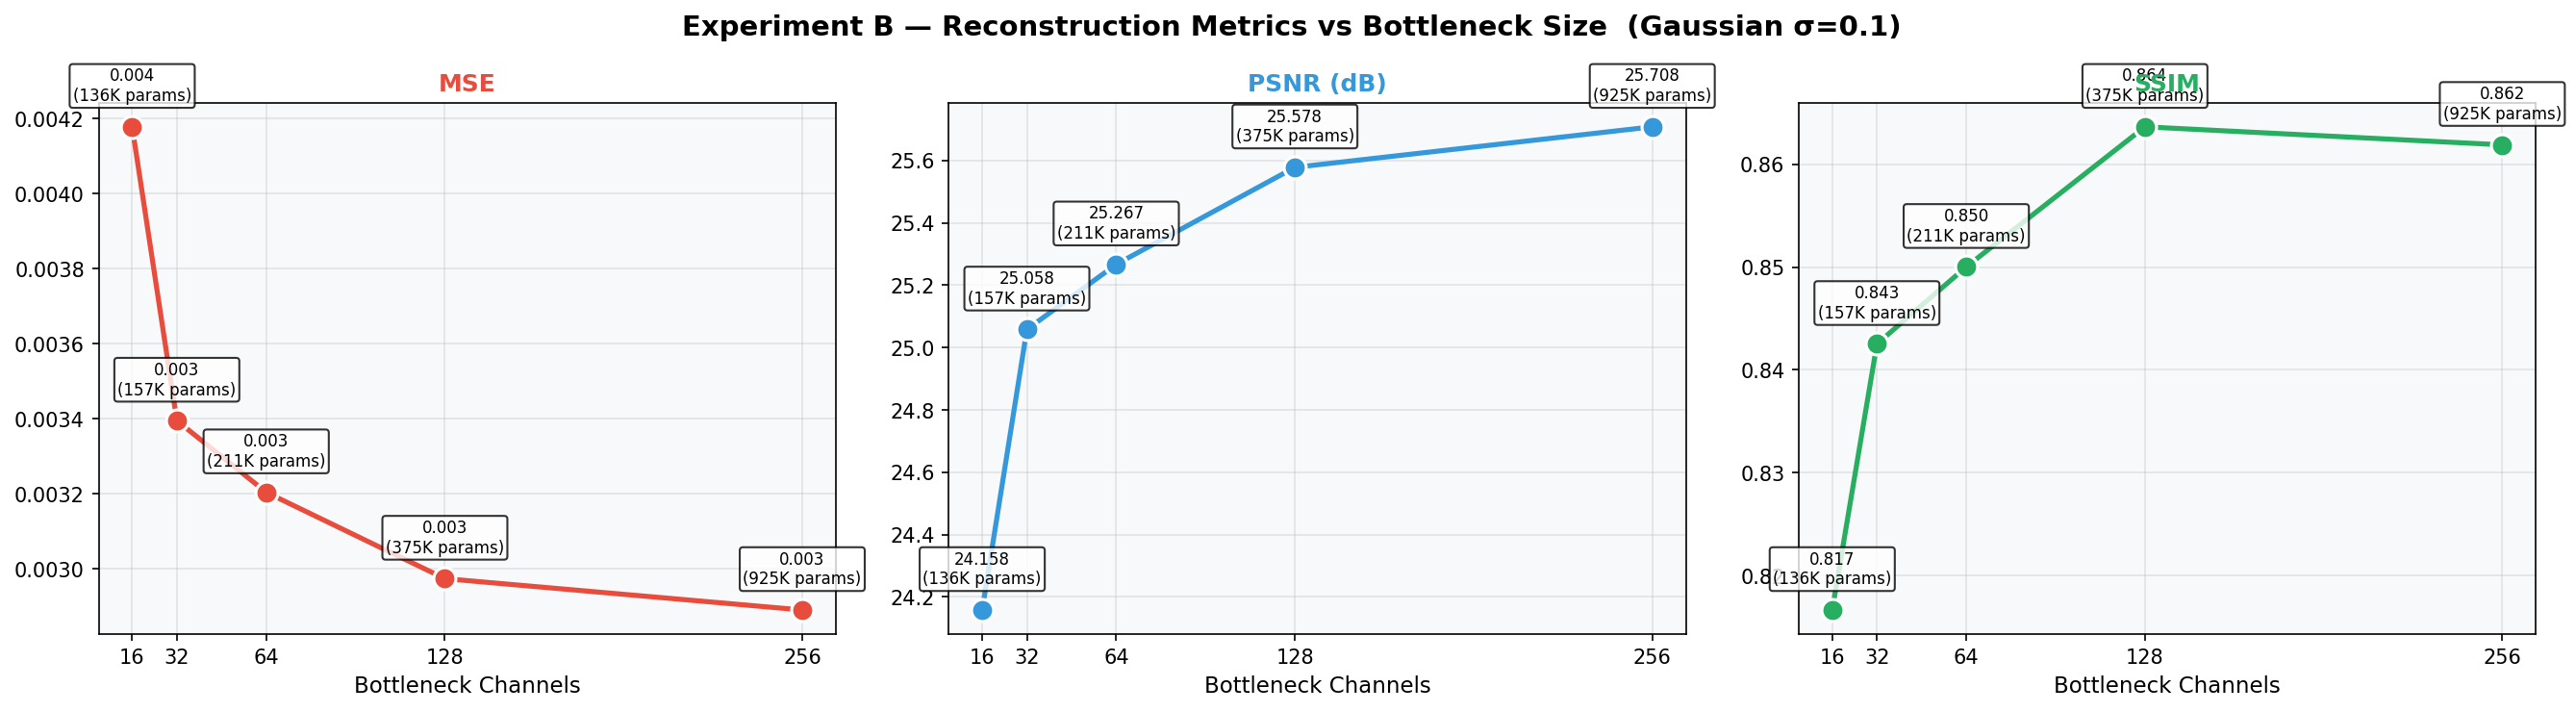
\includegraphics[width=0.95\textwidth]{figures/fig18_exp_B_bottleneck.png}
\caption{Experiment B results: MSE, PSNR, and SSIM vs.\ bottleneck channel count (Gaussian $\sigma=0.1$). Performance improves with capacity but with diminishing returns beyond 128 channels.}
\label{fig:exp_bottleneck}
\end{figure}

\textbf{Key Observations:}
\begin{itemize}[nosep]
    \item Performance improves consistently with bottleneck size, but with diminishing returns.
    \item Going from 128 to 256 channels adds $\sim$59\% more parameters for only a marginal ($\sim$0.3--0.5~dB) PSNR gain.
    \item The \textbf{128-channel bottleneck} offers the best trade-off between model size and denoising quality.
    \item Very small bottlenecks (16~channels) force aggressive compression, acting as a regularizer but losing fine image details.
\end{itemize}

\subsection{PSNR Heatmap}
Figure~\ref{fig:heatmap} presents a grid of PSNR and SSIM values across combinations of Gaussian noise levels and bottleneck sizes.

\begin{figure}[H]
\centering
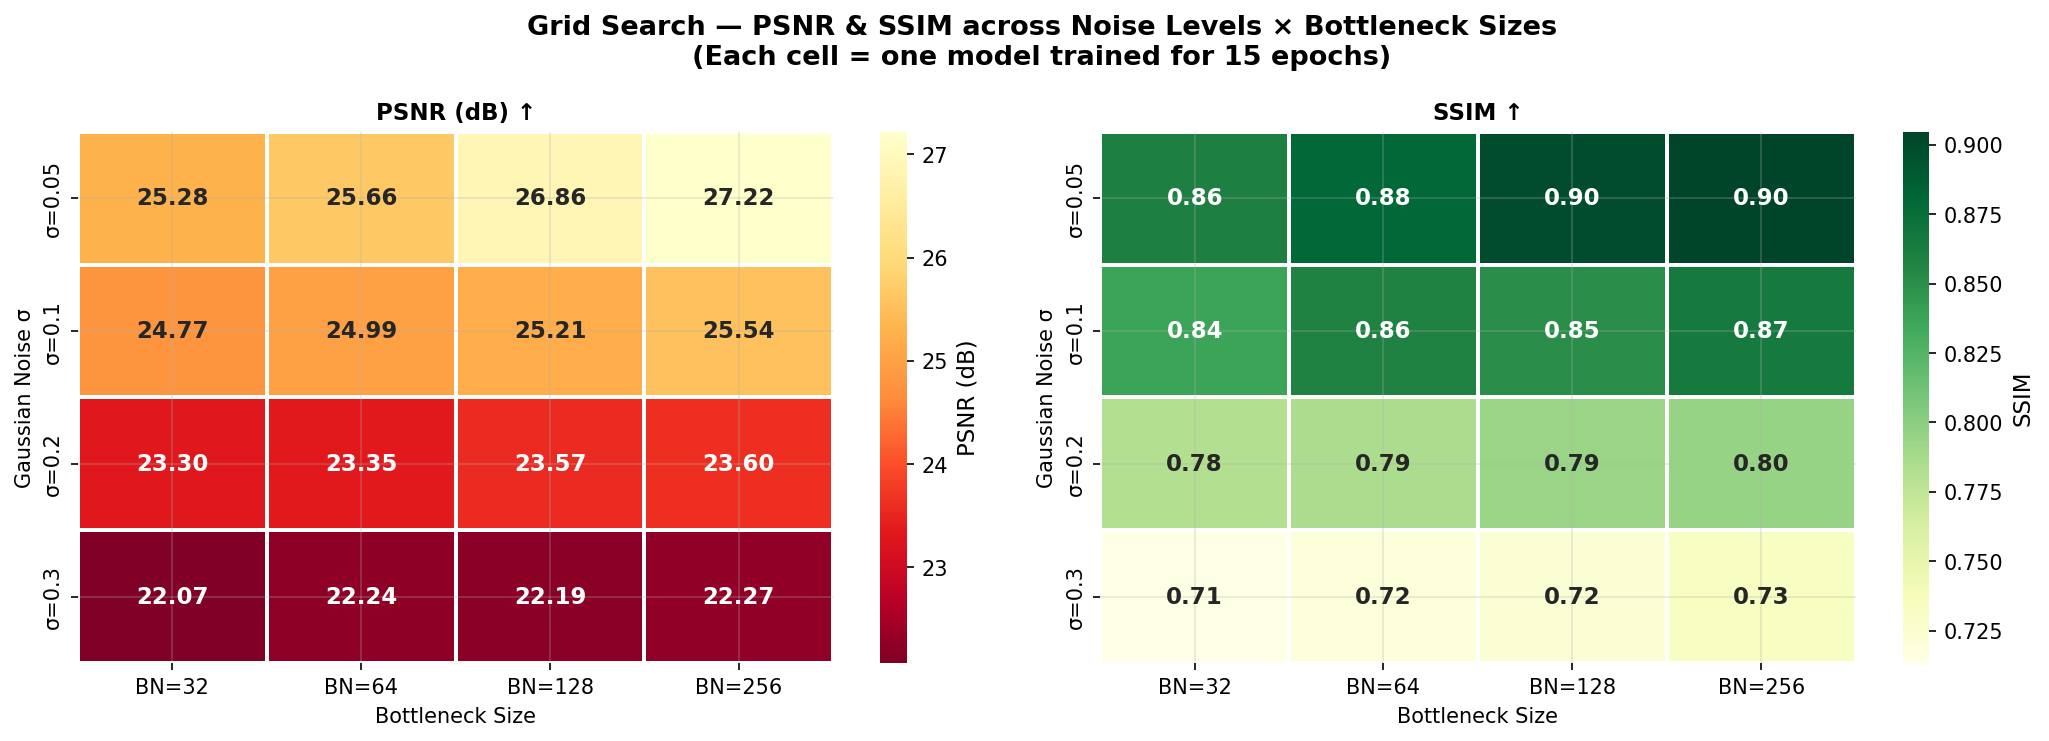
\includegraphics[width=0.70\textwidth]{figures/fig19_heatmaps_psnr_ssim.png}
\caption{PSNR and SSIM heatmaps across Gaussian noise levels ($\sigma$) and bottleneck sizes. The heatmap shows that larger bottlenecks consistently improve performance, but the gains diminish at higher noise levels.}
\label{fig:heatmap}
\end{figure}

\subsection{Multi-Metric Comparison}
Figure~\ref{fig:radar} presents a radar chart comparing model performance across multiple metrics and configurations simultaneously.

\begin{figure}[H]
\centering
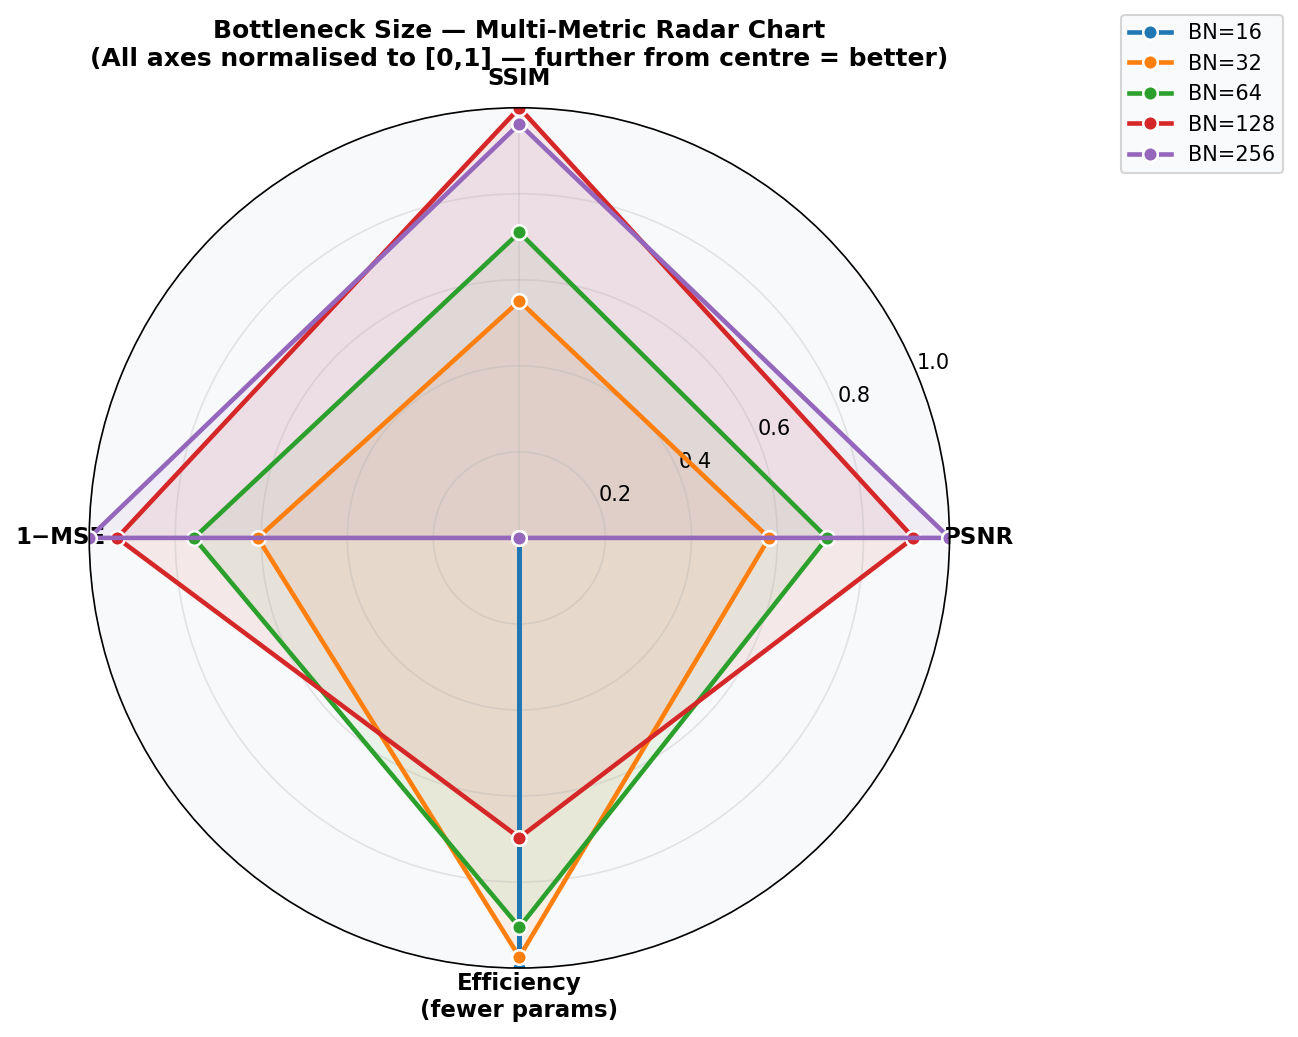
\includegraphics[width=0.70\textwidth]{figures/fig20_radar_chart.png}
\caption{Radar chart comparing reconstruction performance across multiple metrics (MSE, PSNR, SSIM) for different configurations. The 128-channel bottleneck with Gaussian $\sigma=0.1$ achieves the most balanced performance profile.}
\label{fig:radar}
\end{figure}


% ─────────────────────────────────────────────────────────────────────────
% 9. DISCUSSION
% ─────────────────────────────────────────────────────────────────────────
\section{Discussion}
\label{sec:discussion}

\subsection{Model Strengths}
\begin{enumerate}[nosep]
    \item \textbf{Fully convolutional design}: No fully-connected layers means fast inference (even on CPU) and translation-equivariant feature extraction. The model has only $\sim$182K parameters, making it lightweight and efficient.
    \item \textbf{BatchNorm + ReLU stabilization}: Batch normalization after every convolutional layer ensures stable gradient flow and faster convergence (typically $<$30~epochs).
    \item \textbf{Refinement convolutions}: A standard \texttt{Conv2d} after each \texttt{ConvTranspose2d} suppresses the checkerboard artifacts that are common in naïve transposed-convolution upsampling.
    \item \textbf{Mixed-noise capability}: The model handles both Gaussian and salt-and-pepper noise without architectural changes.
    \item \textbf{Sigmoid output}: Constrains pixel values to $[0,1]$ without requiring post-processing clipping.
\end{enumerate}

\subsection{Model Weaknesses}
\begin{enumerate}[nosep]
    \item \textbf{No skip connections}: Unlike U-Net architectures, the model cannot shortcut high-frequency details from encoder to decoder. This limits the preservation of fine textures and edges.
    \item \textbf{Fixed noise distribution}: The model is trained on a specific noise distribution; real-world noise often has spatially-varying statistics, signal-dependent components, or correlated patterns that this model does not capture.
    \item \textbf{Shallow architecture}: With only 3~encoder and 3~decoder blocks, the receptive field is limited. Deeper architectures or attention mechanisms could improve quality on complex textures.
    \item \textbf{MSE-only loss}: Mean squared error penalizes all pixel errors equally and tends to produce blurry outputs. Perceptual losses or adversarial losses could improve visual sharpness.
\end{enumerate}

\subsection{Failure Analysis}
Figure~\ref{fig:failure} highlights the worst-case denoising failures, showing images where the model struggles most.

\begin{figure}[H]
\centering
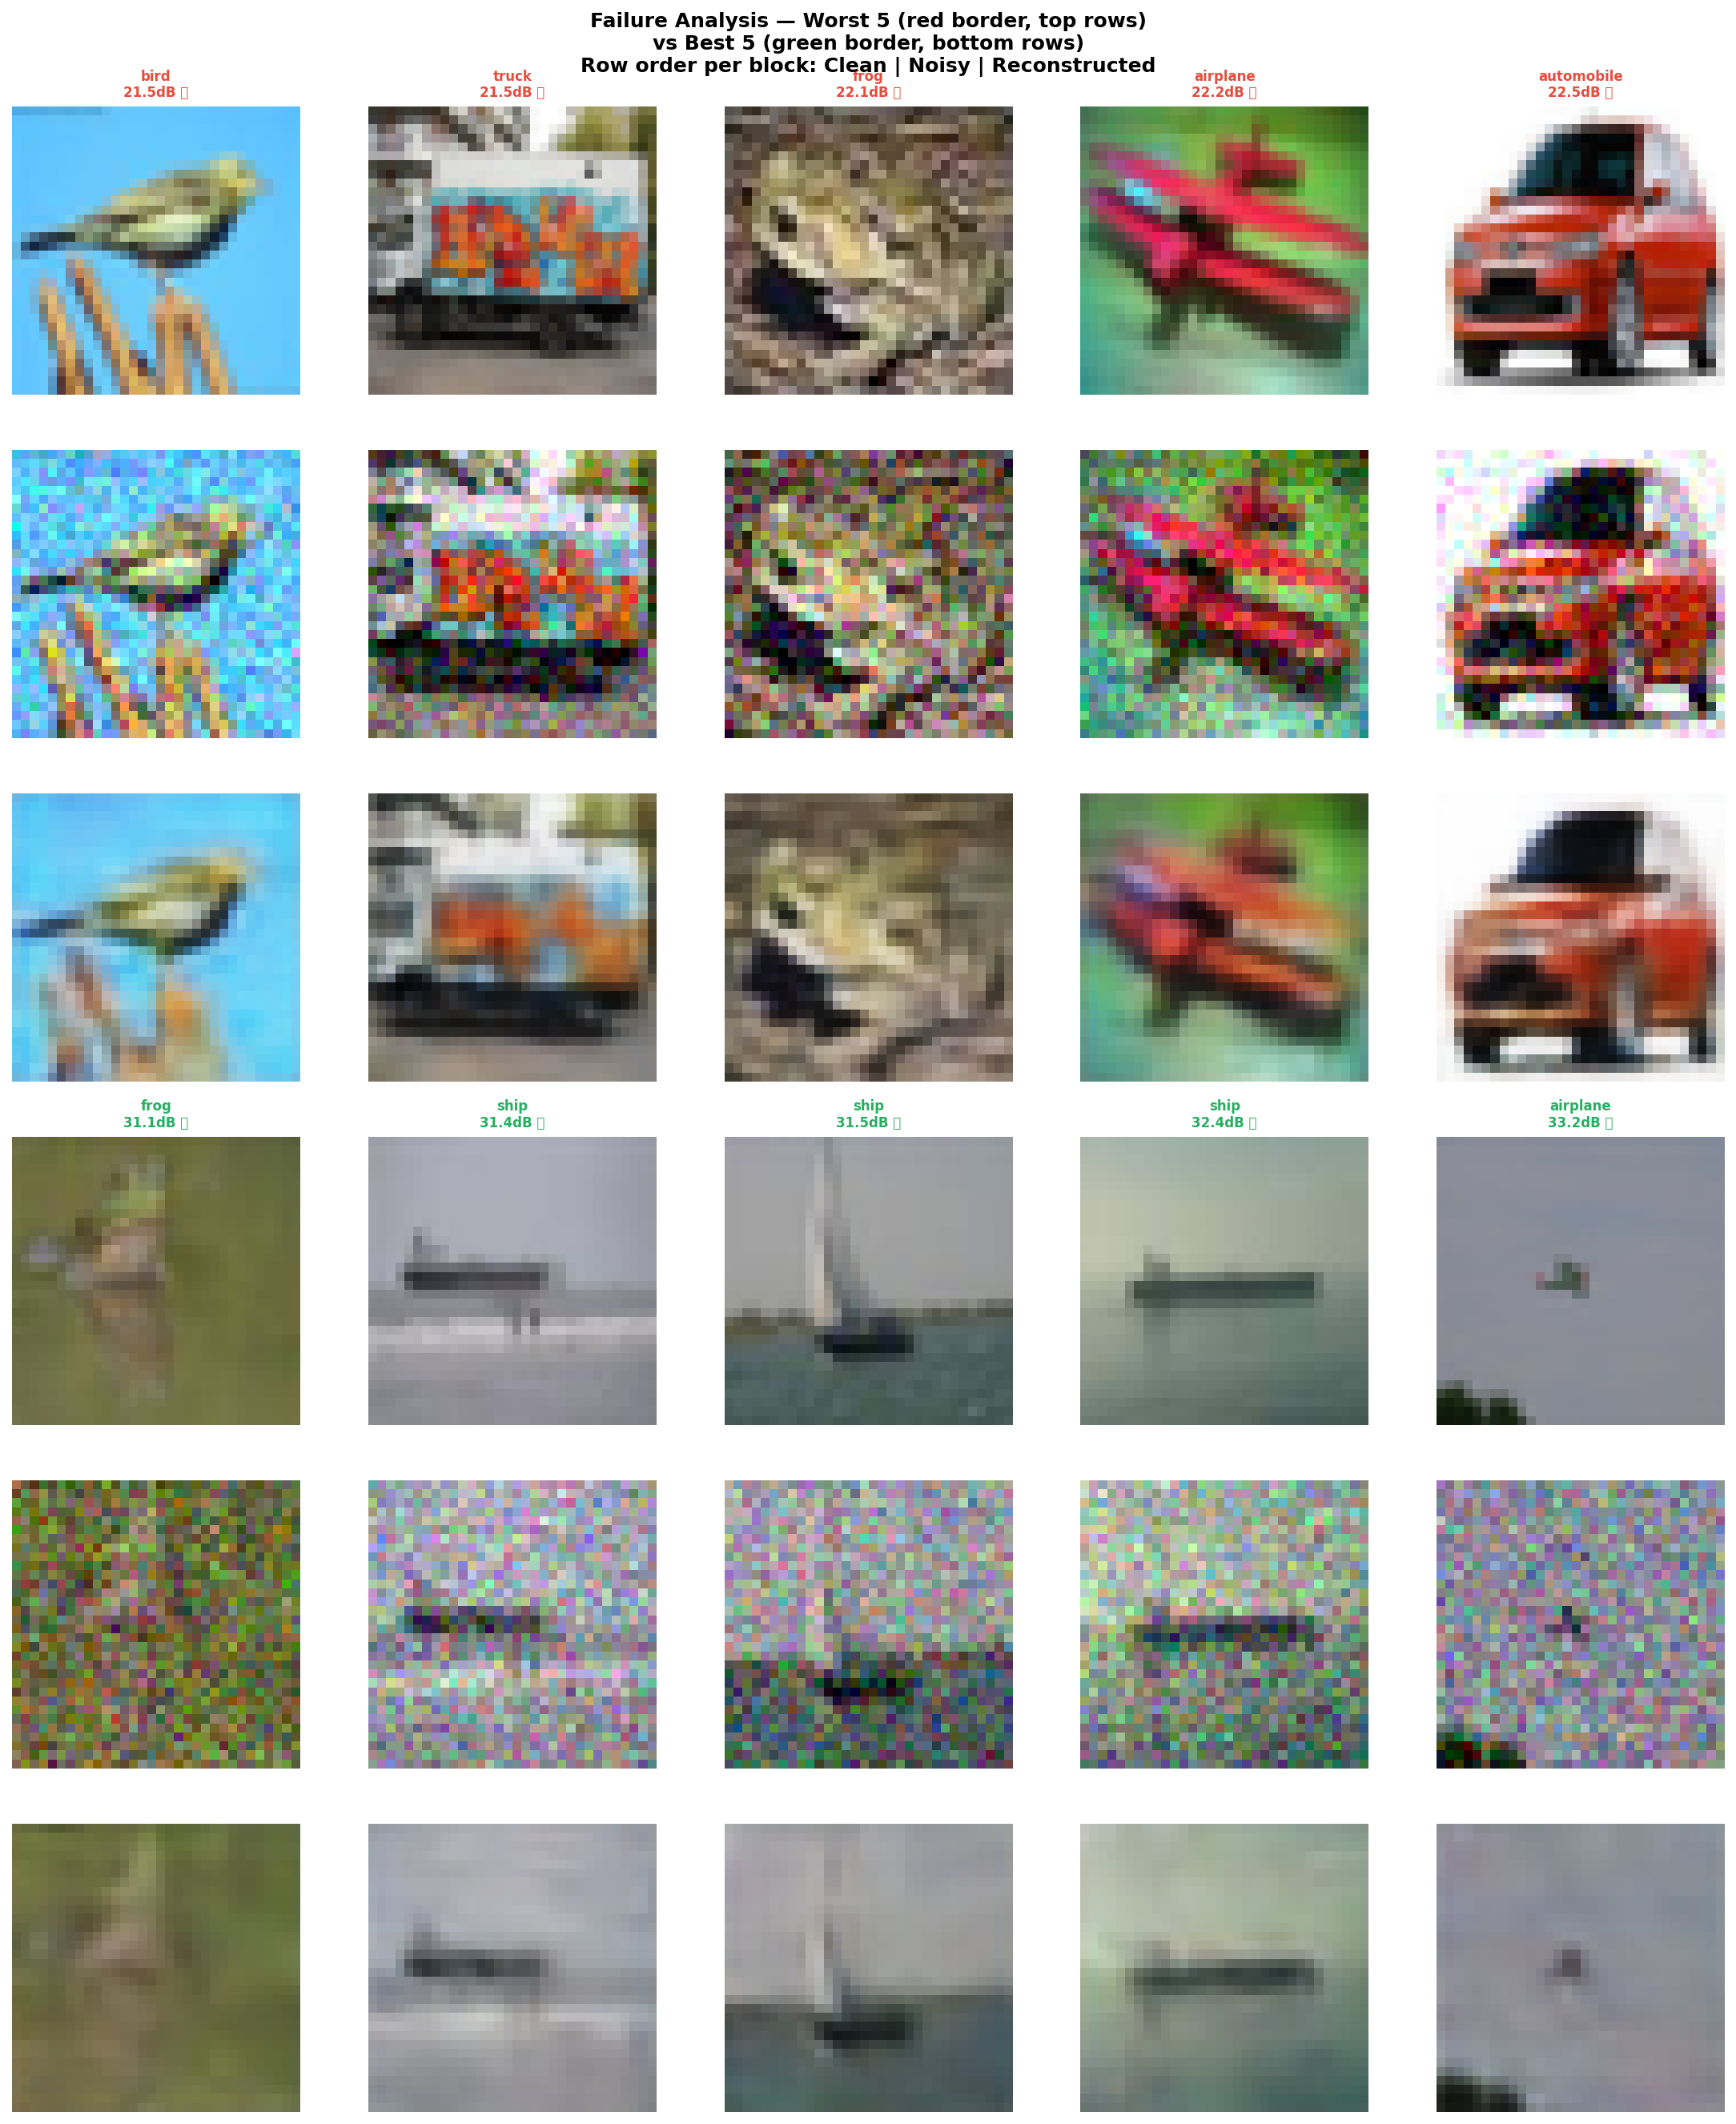
\includegraphics[width=0.90\textwidth]{figures/fig21_failure_analysis.png}
\caption{Failure analysis: examples where the model produces the worst reconstruction quality. Common failure modes include loss of fine texture details (fur, feathers), smeared edges, and color desaturation in images with complex backgrounds.}
\label{fig:failure}
\end{figure}

\subsection{Limitations and Possible Improvements}
\begin{enumerate}[nosep]
    \item \textbf{Skip connections (U-Net style)}: Adding encoder-to-decoder skip connections would allow the decoder to directly access high-resolution features, preserving edges and fine details.
    \item \textbf{Perceptual loss}: Using VGG feature matching loss in addition to MSE would optimize for perceptual similarity rather than pixel-level accuracy, reducing blurriness.
    \item \textbf{Learning rate scheduling}: Cosine annealing or ReduceLROnPlateau could help the model converge to sharper minima and improve final performance.
    \item \textbf{Data augmentation}: Random horizontal flips, crops, and color jitter would increase the effective training set size and improve robustness.
    \item \textbf{Attention mechanisms}: Channel and spatial attention (e.g., CBAM) could help the model focus on informative regions while suppressing noisy areas.
    \item \textbf{Noise-level conditioning}: Providing the noise level as an additional input to the network (e.g., via FiLM layers) would allow a single model to handle variable noise levels without retraining.
\end{enumerate}


% ─────────────────────────────────────────────────────────────────────────
% 10. CONCLUSION
% ─────────────────────────────────────────────────────────────────────────
\section{Conclusion}
\label{sec:conclusion}

This report presented a convolutional Denoising Autoencoder for image denoising on the CIFAR-10 dataset. The model achieves a PSNR of 24.62~dB and SSIM of 0.8225 on the test set with Gaussian noise $\sigma=0.1$, demonstrating effective noise removal with only 181{,}591 parameters. Our experimental study demonstrates that:
\begin{itemize}[nosep]
    \item Increasing noise levels degrades reconstruction quality, with Gaussian noise being harder to remove than salt-and-pepper noise (21.70~dB vs.~23.07~dB at the 0.30 level).
    \item Salt-and-pepper noise is comparatively easier to denoise because it is spatially sparse---intact neighboring pixels provide strong reconstruction cues.
    \item Larger bottleneck sizes improve performance but with diminishing returns; the 128-channel bottleneck offers the best cost--quality trade-off (24.07~dB PSNR with 181K params vs.~24.45~dB with 288K params).
\end{itemize}

The comprehensive statistical analysis of CIFAR-10 (Section~\ref{sec:statistics}) provided valuable insights into the dataset's characteristics, including its balanced class distribution, non-normal pixel distributions, strong inter-channel correlations, and the low-dimensional manifold structure revealed by PCA and t-SNE.

Figure~\ref{fig:final_comparison} demonstrates the final denoising quality on both noise types, and Figure~\ref{fig:results_dashboard} presents a comprehensive results dashboard.

\begin{figure}[H]
\centering
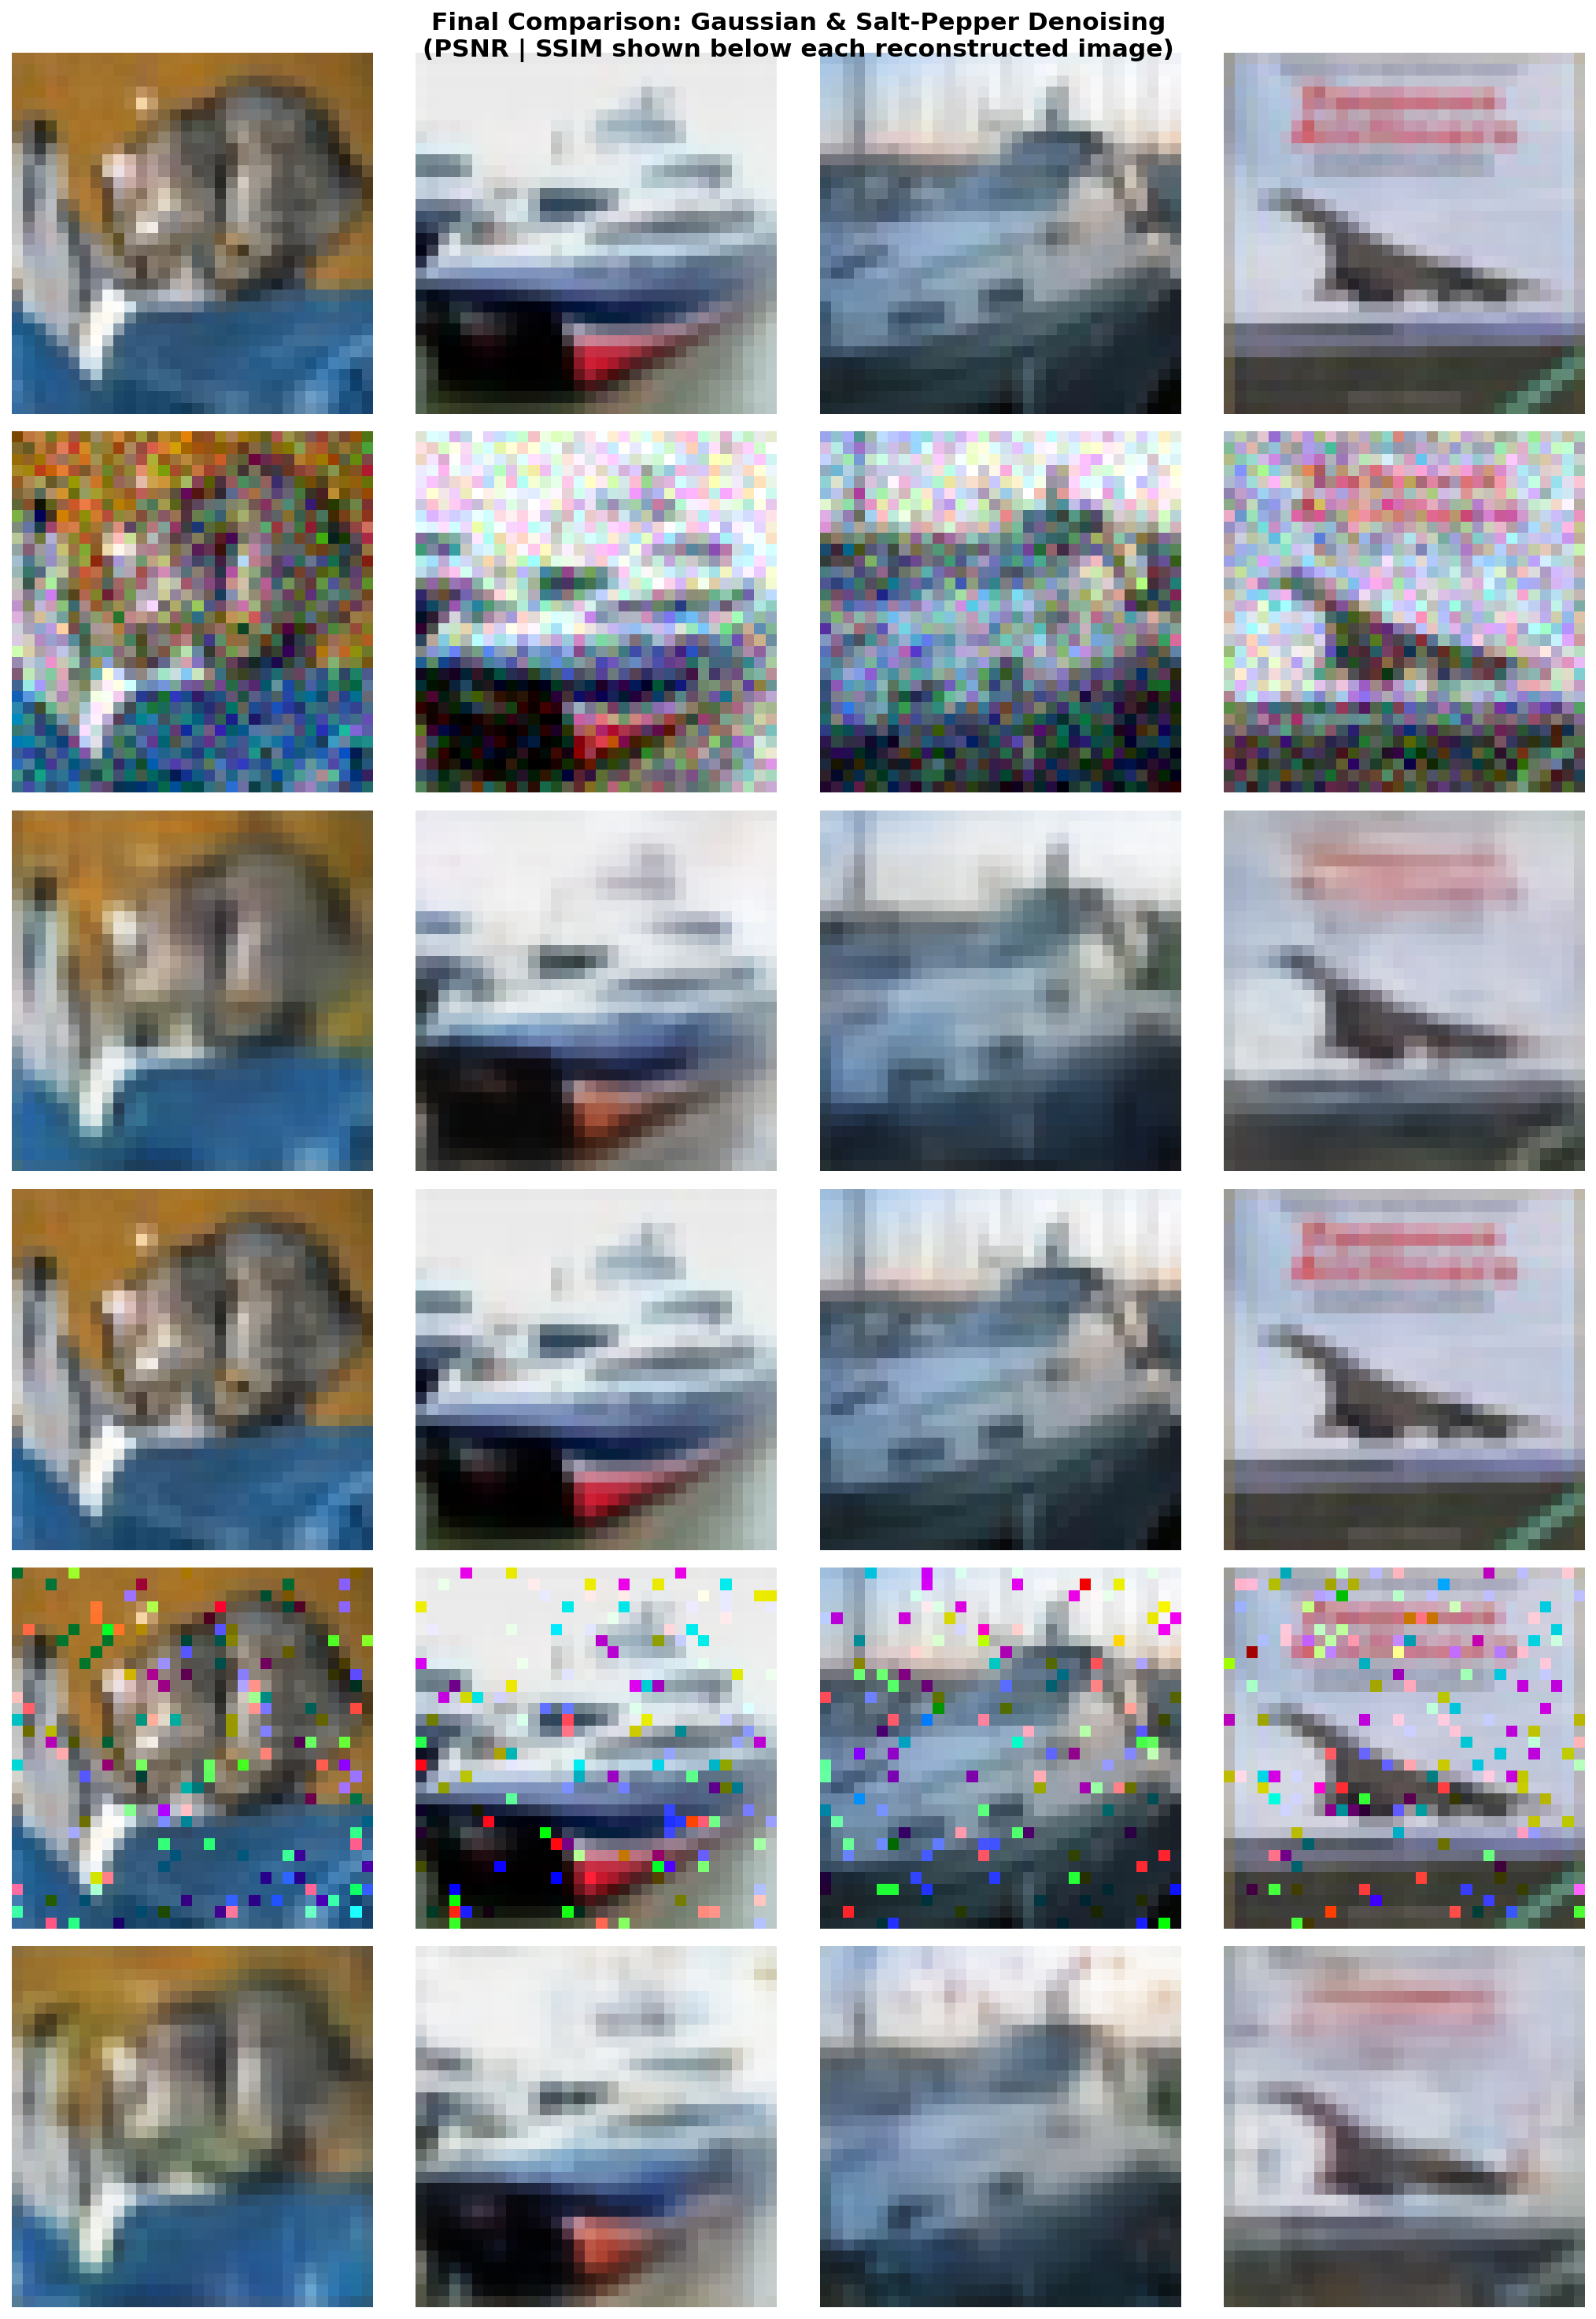
\includegraphics[width=0.95\textwidth]{figures/fig22_final_comparison.png}
\caption{Final comparison: Gaussian (top) and salt-and-pepper (bottom) denoising results showing clean, noisy, and reconstructed images.}
\label{fig:final_comparison}
\end{figure}

\begin{figure}[H]
\centering
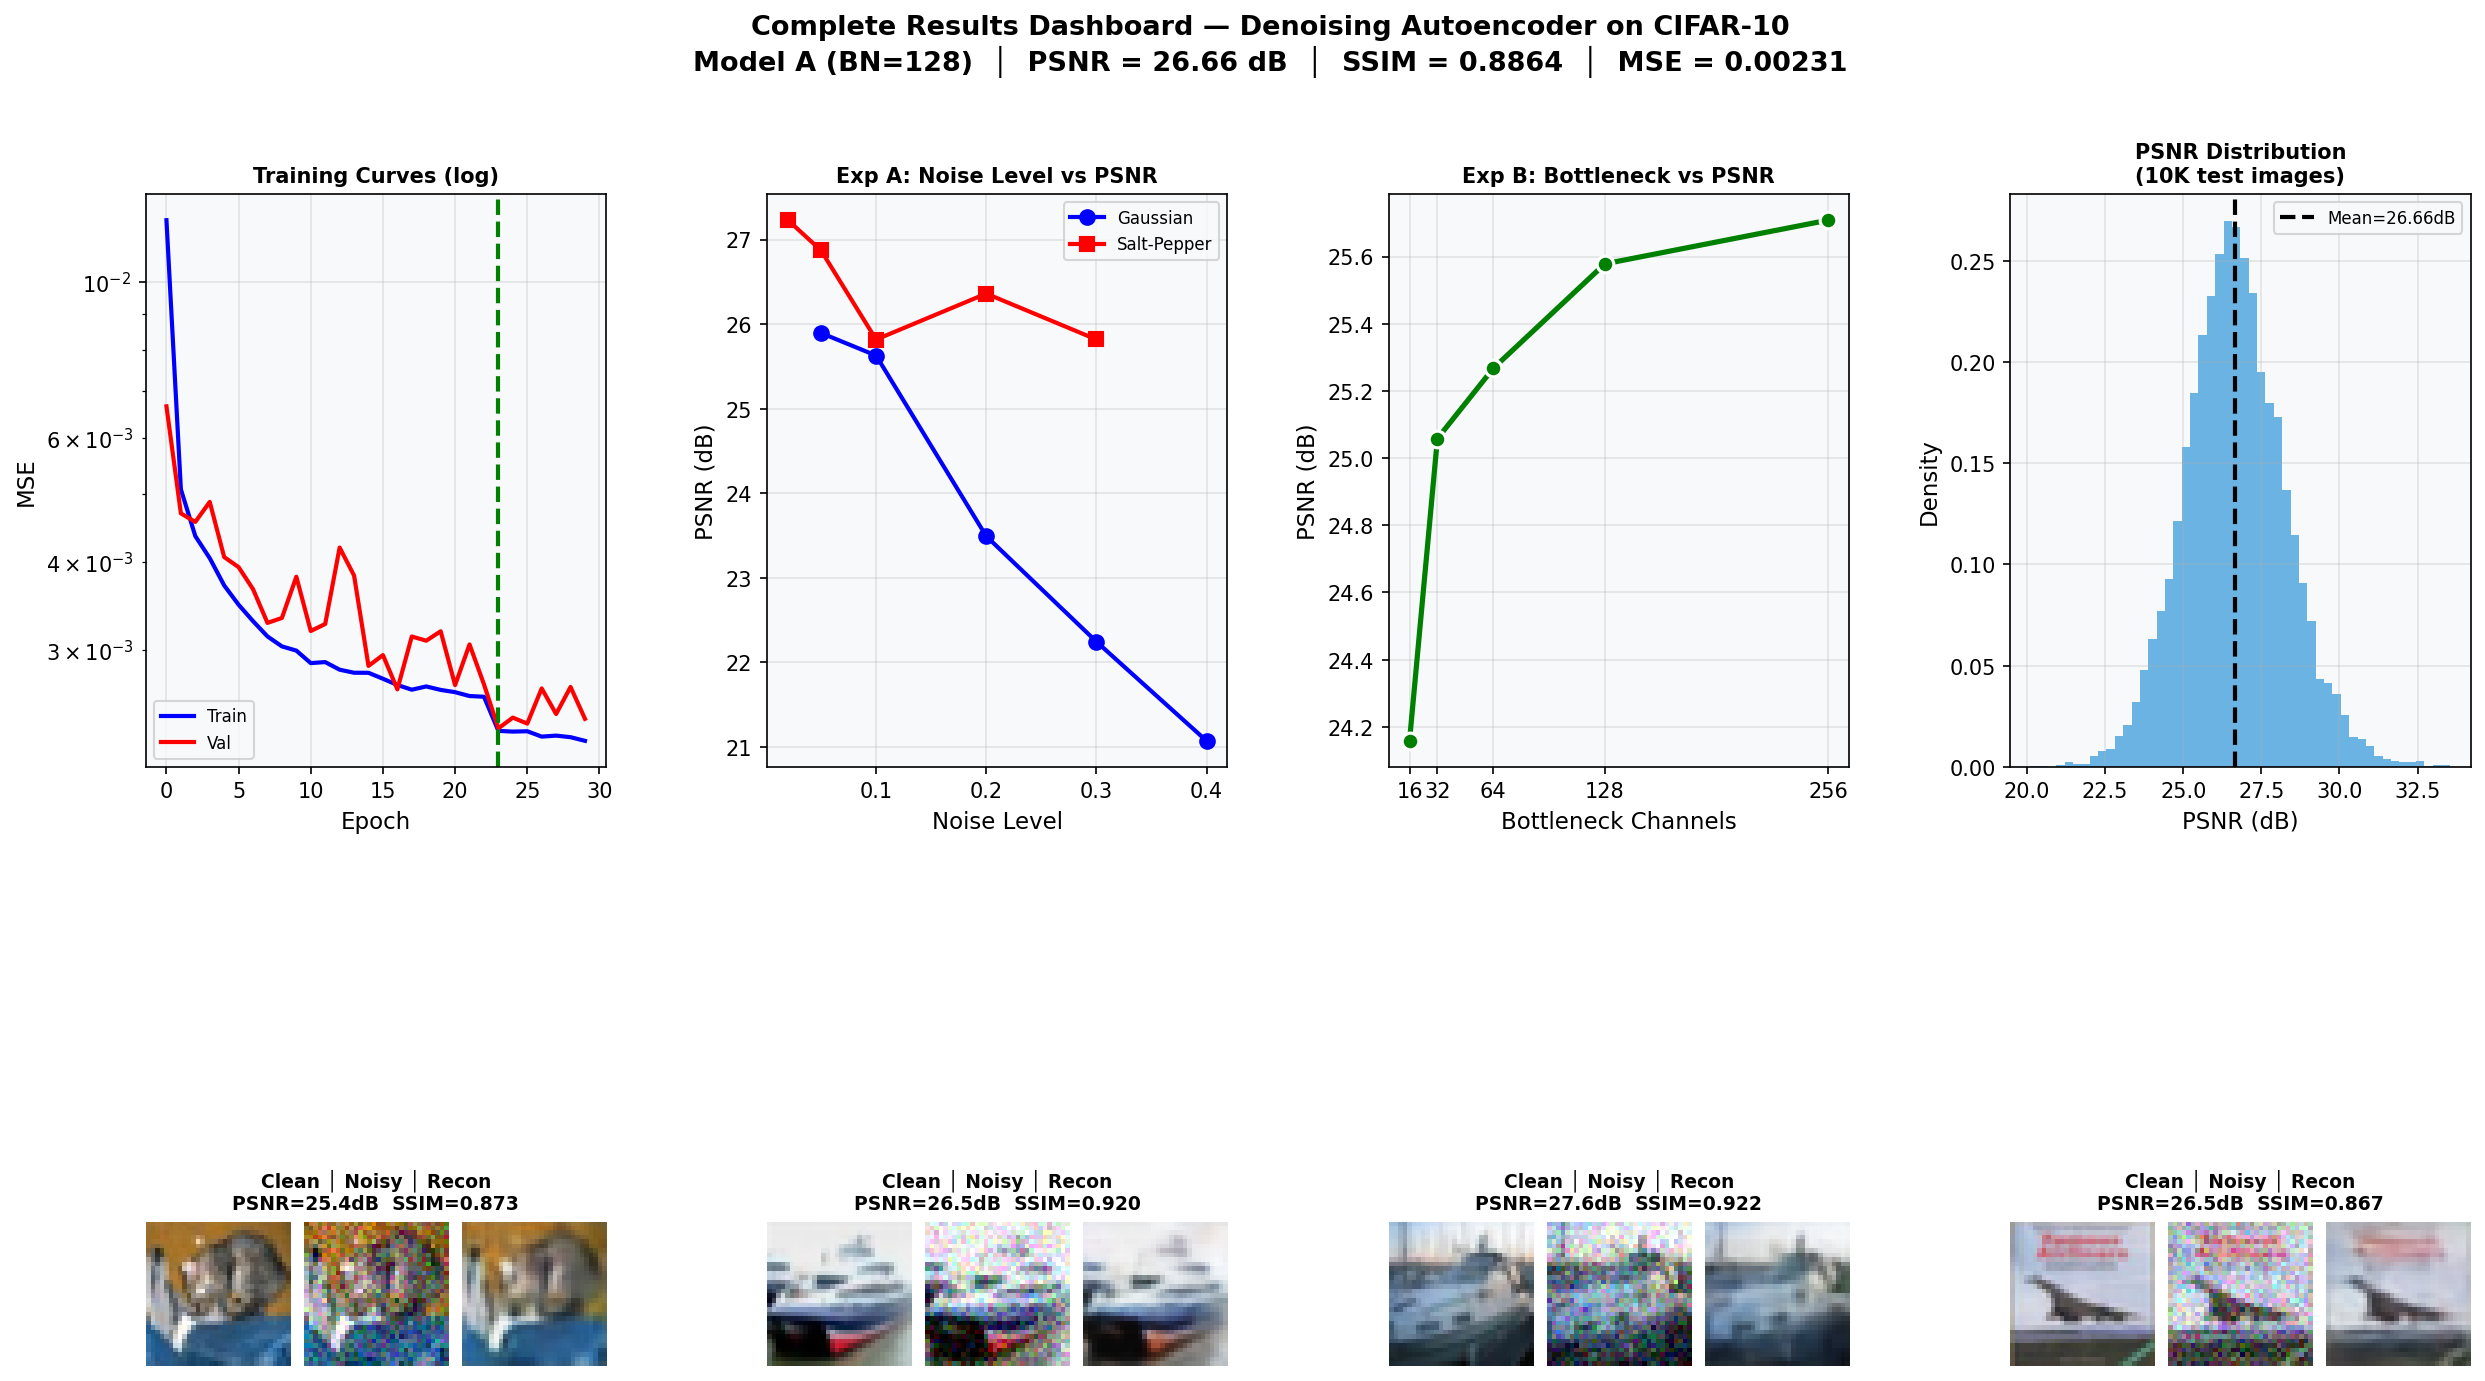
\includegraphics[width=0.95\textwidth]{figures/fig23_results_dashboard.png}
\caption{Comprehensive results dashboard summarizing key metrics, training curves, and denoising performance in a single view.}
\label{fig:results_dashboard}
\end{figure}

Future work could explore U-Net architectures with skip connections, perceptual losses, and attention mechanisms to further improve denoising quality, especially at high noise levels.


% ─────────────────────────────────────────────────────────────────────────
% REFERENCES
% ─────────────────────────────────────────────────────────────────────────
\begin{thebibliography}{9}

\bibitem{vincent2008extracting}
Vincent, P., Larochelle, H., Bengio, Y., Manzagol, P.A.:
Extracting and composing robust features with denoising autoencoders.
In: Proceedings of the 25th International Conference on Machine Learning (ICML), pp. 1096--1103 (2008)

\bibitem{krizhevsky2009learning}
Krizhevsky, A.:
Learning multiple layers of features from tiny images.
Technical Report, University of Toronto (2009)

\bibitem{kingma2014adam}
Kingma, D.P., Ba, J.:
Adam: A method for stochastic optimization.
In: Proceedings of the 3rd International Conference on Learning Representations (ICLR) (2015)

\bibitem{goodfellow2016deep}
Goodfellow, I., Bengio, Y., Courville, A.:
Deep Learning.
MIT Press (2016)

\bibitem{ronneberger2015u}
Ronneberger, O., Fischer, P., Brox, T.:
U-Net: Convolutional networks for biomedical image segmentation.
In: Medical Image Computing and Computer-Assisted Intervention (MICCAI), pp. 234--241 (2015)

\bibitem{zhang2017beyond}
Zhang, K., Zuo, W., Chen, Y., Meng, D., Zhang, L.:
Beyond a Gaussian denoiser: Residual learning of deep CNN for image denoising.
IEEE Transactions on Image Processing, 26(7), 3142--3155 (2017)

\bibitem{wang2004image}
Wang, Z., Bovik, A.C., Sheikh, H.R., Simoncelli, E.P.:
Image quality assessment: from error visibility to structural similarity.
IEEE Transactions on Image Processing, 13(4), 600--612 (2004)

\bibitem{maaten2008tsne}
Van der Maaten, L., Hinton, G.:
Visualizing data using t-SNE.
Journal of Machine Learning Research, 9, 2579--2605 (2008)

\bibitem{jolliffe2016pca}
Jolliffe, I.T., Cadima, J.:
Principal component analysis: a review and recent developments.
Philosophical Transactions of the Royal Society A, 374(2065), 20150202 (2016)

\end{thebibliography}

\end{document}
